\documentclass[12pt]{article} %***
\usepackage[sectionbib]{natbib}
\usepackage{array,epsfig,fancyheadings,rotating}
\usepackage[]{hyperref}  %<----modified by Ivan
%%%%%%%%%%%%%%%%%%%%%%%%%%%%%%%%%%%%
\usepackage{sectsty, secdot}
%\sectionfont{\fontsize{12}{15}\selectfont}
\sectionfont{\fontsize{12}{14pt plus.8pt minus .6pt}\selectfont}
\renewcommand{\theequation}{\thesection\arabic{equation}}
\subsectionfont{\fontsize{12}{14pt plus.8pt minus .6pt}\selectfont}
%%%%%%%%%%%%%%%%%%%%%%%%%%%%%%%%%%%%%%%%%%%%%%%%%%%%%%%%%%%%%%%%%%%%%%%%%%%%%%%%%%%%%%%%

\textwidth=31.9pc
\textheight=46.5pc
\oddsidemargin=1pc
\evensidemargin=1pc
\headsep=15pt
%\headheight=.2cm
\topmargin=.6cm
\parindent=1.7pc
\parskip=0pt

\usepackage{amsmath}
\usepackage{amssymb}
\usepackage{amsfonts}
\usepackage{multirow}
\usepackage{amsthm}
\usepackage[title]{appendix}

\usepackage{bm}
\usepackage{graphicx}
\usepackage{color}
\usepackage{booktabs}
\usepackage{algorithm}
\usepackage{algorithmic}
\usepackage{IEEEtrantools}
\usepackage{enumerate}



\DeclareMathOperator{\mytr}{tr}
\DeclareMathOperator{\mydiag}{diag}
\DeclareMathOperator{\myrank}{Rank}
\DeclareMathOperator{\myE}{E}
\DeclareMathOperator{\myVar}{Var}
\DeclareMathOperator*{\argmax}{arg\,max}
\DeclareMathOperator*{\argmin}{arg\,min}

\newcommand{\bQ}{\mathbf{Q}}
\newcommand{\bM}{\mathbf{M}}
\newcommand{\bZ}{\mathbf{Z}}
\newcommand{\bA}{\mathbf{A}}
\newcommand{\bB}{\mathbf{B}}
\newcommand{\bE}{\mathbf{E}}
\newcommand{\bF}{\mathbf{F}}
\newcommand{\bX}{\mathbf{X}}
\newcommand{\bP}{\mathbf{P}}
\newcommand{\bY}{\mathbf{Y}}
\newcommand{\bH}{\mathbf{H}}
\newcommand{\bG}{\mathbf{G}}
\newcommand{\bJ}{\mathbf{J}}
\newcommand{\bC}{\mathbf{C}}
\newcommand{\bO}{\mathbf{O}}
\newcommand{\bR}{\mathbf{R}}
\newcommand{\bI}{\mathbf{I}}
\newcommand{\bU}{\mathbf{U}}
\newcommand{\bD}{\mathbf{D}}
\newcommand{\bV}{\mathbf{V}}
\newcommand{\bW}{\mathbf{W}}
\newcommand{\bL}{\mathbf{L}}

\newcommand{\bu}{\mathbf{u}}
\newcommand{\bw}{\mathbf{w}}

\newcommand{\ud}{\mathbf{d}}

\newcommand{\bfsym}[1]{\ensuremath{\boldsymbol{#1}}}
\def\blambda {\bfsym {\lambda}} 
\def\bLambda {\bfsym {\Lambda}} 
\def\bSigma {\bfsym {\Sigma}} 
\def\bTheta {\bfsym {\Theta}} 
\def\bPsi {\bfsym {\Psi}} 





\newtheorem{assumption}{Assumption}

\setcounter{page}{1}
\newtheorem{theorem}{Theorem}
\newtheorem{lemma}{Lemma}
\newtheorem{corollary}{Corollary}
\newtheorem{proposition}{Proposition}
\theoremstyle{definition}
\newtheorem{definition}{Definition}
%\newtheorem{proof}{Proof}
\newtheorem{example}{Example}
\newtheorem{remark}{Remark}
\pagestyle{fancy}

%%%%%%%%%%%%%%%%%%%%%%%%%%%%%%%%%%%%%%%%%%%%%%%%%%%%%%%%%%%%%%%%%%%%%%%%%%%%%%%%%%%%%%%%%%%%%%%%%%%%%%%%%%%%%%%%%%%%%%%%%%%%
\pagestyle{fancy}
\def\n{\noindent}
\lhead[\fancyplain{} \leftmark]{}
\chead[]{}
\rhead[]{\fancyplain{}\rightmark}
\cfoot{}
%\headrulewidth=0pt  %<-modified by Ivan

%%%%%%%%%%%%%%%%%%%%%%%%%%%%%%%%%%%%%%%%%%%%%%%%%%%%%%%%%%%%%%%%%%%%%%%%%%%%%%%%%%%%%%%%%%%%%%%%%%%%%%%%%%%%%%%%%%%%%%%%%%%%
%%%%%%%%%%%%%%%%%%%%%%%%%%%%%%%%%%%%%%%%%%%%%%%%%%%%%%%%%%%%%%%%%%%%%%%%%%%%%%%%%%%%%%%%%%%%%%%%%%%%%%%%%%%%%%%%%%%%%%%%%%%%

\begin{document}

%%%%%%%%%%%%%%%%%%%%%%%%%%%%%%%%%%%%%%%%%%%%%%%%%%%%%%%%%%%%%%%%%%%%%%%%%%%%%%%%%%%%%%%%%%%%%%%%%%%%%%%%%%%%%%%%%%%%%%%%%%%%
%%%%%%%%%%%%%%%%%%%%%%%%%%%%%%%%%%%%%%%%%%%%%%%%%%%%%%%%%%%%%%%%%%%%%%%%%%%%%%%%%%%%%%%%%%%%%%%%%%%%%%%%%%%%%%%%%%%%%%%%%%%%

\renewcommand{\baselinestretch}{2}

\markright{ \hbox{\footnotesize\rm Statistica Sinica
%{\footnotesize\bf 24} (201?), 000-000
}\hfill\\[-13pt]
\hbox{\footnotesize\rm
%\href{http://dx.doi.org/10.5705/ss.20??.???}{doi:http://dx.doi.org/10.5705/ss.20??.???}
}\hfill }

\markboth{\hfill{\footnotesize\rm Rui Wang AND Xingzhong Xu} \hfill}
{\hfill {\footnotesize\rm LEAST FAVORABLE DIRECTION TEST} \hfill}

\renewcommand{\thefootnote}{}
$\ $\par

%%%%%%%%%%%%%%%%%%%%%%%%%%%%%%%%%%%%%%%%%%%%%%%%%%%%%%%%%%%%%%%%%%%%%%%%%%%%%%%%%%%%%%%%%%%%%%%%%%%%%%%%%%%%%%%%%%%%%%%%%%%%

\fontsize{12}{14pt plus.8pt minus .6pt}\selectfont \vspace{0.8pc}
\centerline{\large\bf LEAST FAVORABLE DIRECTION TEST FOR }
\vspace{2pt} \centerline{\large\bf MULTIVARIATE ANALYSIS OF VARIANCE}
\vspace{2pt} \centerline{\large\bf IN HIGH DIMENSION}
\vspace{.4cm} \centerline{
    Rui Wang, Xingzhong Xu
} \vspace{.4cm} \centerline{\it
Beijing Institute of Technology
}
 \vspace{.55cm} \fontsize{9}{11.5pt plus.8pt minus
.6pt}\selectfont

%%%%%%%%%%%%%%%%%%%%%%%%%%%%%%%%%%%%%%%%%%%%%%%%%%%%%%%%%%%%%%%%%%%%%%%%%%%%%%%%%%%%%%%%%%%%%%%%%%%%%%%%%%%%%%%%%%%%%%%%%%%%

\begin{quotation}
\noindent {\it Abstract:}
This paper considers the problem of multivariate analysis of variance for normal samples.
    When the sample dimension is larger than the sample size, the classical likelihood ratio test is not defined since the likelihood function is unbounded.
    Based on the unboundedness of the likelihood function, we propose a new test called least favorable direction test.
    The asymptotic distributions of the test statistic are derived under both nonspiked and spiked covariances.
    The local asymptotic power function of the test is also given.
    %{\color{red}
    %These asymptotic results also hold under spiked covariance matrix which can characterize the strong correlations between variables.
%}
    The asymptotic power function and simulations show that the proposed test has particular high power when variables are strongly correlated.

\vspace{9pt}
    \noindent {\it Key words and phrases:}
    High dimensional data, least favorable direction test, multivariate analysis of variance, principal component analysis, spiked covariance.
%Balanced incomplete block design, Hadamard matrix, nearly balanced incomplete block design, orthogonal array.
\par
\end{quotation}\par



\def\thefigure{\arabic{figure}}
\def\thetable{\arabic{table}}

\renewcommand{\theequation}{\thesection.\arabic{equation}}


\fontsize{12}{14pt plus.8pt minus .6pt}\selectfont

\setcounter{section}{1} %***
\setcounter{equation}{0} %-1
\noindent {\bf 1. Introduction}

Suppose there are $k$ ($k\geq 2$) independent samples of $p$-dimensional data.
Within the $i$th sample ($1\leq i\leq k$), the observations $\{X_{ij}\}_{j=1}^{n_i}$ are independent and identically distributed (iid) as $\mathcal{N}_p(\theta_i,\bSigma)$, the $p$-dimensional normal distribution with mean vector $\theta_i$ and common variance matrix $\bSigma$.
%Suppose there are $k$ normal populations with possibly different means $\theta_1,\ldots,\theta_k$, but all with the same variance $\bSigma$.
%Suppose we observe $k$ independent random samples, each from the distribution $\mathcal{N}_p(\theta_i,\bSigma)$, where $1\leq i\leq k$, $k\geq 2$ is a fixed constant, $\theta_i$ and $\bSigma$ are unknown parameters.
%Denote by $X_{ij}\in \mathbb{R}^p$ the $j$th observation in group $i$, $j=1,\ldots,n_i$, $i=1,\ldots, k$,  where $n_i$ is the samples size of group $i$, $1\leq i \leq k$.
We would like to test the hypotheses
\begin{equation}\label{hypothesis}
    H_0: \theta_1=\theta_2=\cdots=\theta_k\quad \text{v.s.}\quad H_1: \text{$\theta_i\neq \theta_j$ for some $i\neq j$}.
\end{equation}
This testing problem is known as one-way multivariate analysis of variance (MANOVA) and has been well studied when $p$ is small compared with $N$, where $N=\sum_{i=1}^k n_i$ is the total sample size.

Let $\bH=\sum_{i=1}^k n_i (\bar{\bX}_i-\bar{\bX})(\bar{\bX}_i-\bar{\bX})^\top$ be the sum-of-squares between groups and $\bG=\sum_{i=1}^k \sum_{j=1}^{n_i}(X_{ij}-\bar{\bX}_i)(X_{ij}-\bar{\bX}_i)^\top$ be the sum-of-squares within groups, where $\bar{\bX}_i=n_i^{-1}\sum_{j=1}^{n_i}X_{ij}$ is the sample mean of group $i$ and $\bar{\bX}=N^{-1}\sum_{i=1}^k\sum_{j=1}^{n_i}X_{ij}$ is the pooled sample mean.
   There are four classical test statistics for hypotheses~\eqref{hypothesis}, which are all based on the eigenvalues of $\bH\bG^{-1}$. 


       \begin{center}
       \begin{tabular}{|cc|}
           \hline
       {Wilks' Lambda:} & $|\bG+\bH|/|\bG|$\\
       {Pillai trace:} & $\mytr[\bH(\bG+\bH)^{-1}]$\\
       {Hotelling-Lawley trace:} & $\mytr[\bH \bG^{-1}]$\\
       {Roy's maximum root:} & $\lambda_{1}(\bH \bG^{-1})$\\
           \hline
           \end{tabular}
       \end{center}

%There are four classical tests for hypothesis~\eqref{hypothesis}: Wilks' Lambda (which is also the LRT), Hotelling-Lawley trace, Pillai Trace and Roy's maximum root.


In some modern scientific applications, people would like to test hypotheses~\eqref{hypothesis} in high dimensional setting, i.e., $p$ is greater than $N$.
See, for example,~\citet{Verstynen1209} and~\citet{Tsai2009}.
%However, when $p>n-k$, the LRT for hypothesis~\eqref{hypothesis} is not well defined.
However, when $p\geq N$, the four classical test statistics are all not defined.
  Researchers have done extensive work to study the testing problem~\eqref{hypothesis} in high dimensional setting.
 So far, most tests are designed for two-sample case, i.e., $k=2$.
  See, for example,~\citet{Bai1996Efiect},~\cite{Srivastava2007Multivariate},~\citet{Chen2010A},~\citet{Tony2013} and \citet{Feng2014Two}.
  Recently, some tests have also been introduced for the case of general $k$.~\cite{Schott2007Some} modified Hotelling-Lawley trace and proposed the test statistic
  %$$
  %T_{SC}=\frac{1}{\sqrt{n-1}}\big(
  %\frac{1}{k-1}\mytr\big(\sum_{i=1}^k n_i\bar{X}_i\bar{X}_i^\top-n\bar{X}\bar{X}^\top\big)-\frac{1}{n-k}\mytr\big(\sum_{i=1}^k \sum_{j=1}^{n_i}X_{ij}X_{ij}^\top-\sum_{i=1}^k n_i\bar{X}_i\bar{X}_i^\top\big)
  %\big),
  %$$
  %where $\bar{\bX}_i=n_i^{-1}\sum_{j=1}^{n_i}X_{ij}$ and $\bar{\bX}=n^{-1}\sum_{i=1}^k\sum_{j=1}^{n_i}X_{ij}$.
  $$
  T_{Sc}=\frac{1}{\sqrt{N-1}}\Big(
  \frac{1}{k-1}\mytr\big(\bH\big)-\frac{1}{N-k}\mytr\big(\bG\big)
  \Big).
  $$
Statistic $T_{Sc}$ is a representative of the so-called sum-of-squares type statistics as it is based on an estimation of squared Euclidean norm $\sum_{i=1}^k n_i\|\theta_i-\bar{\theta}\|^2$, where $\bar{\theta}=N^{-1}\sum_{i=1}^k n_i \theta_i$.
See~\cite{Srivastava2013},~\cite{Hu2017},~\cite{Yamada2015},~\cite{ZHANG2017200},~\cite{Chang2017} and~\cite{2017arXiv171007878C} for some other sum-of-squares type test statistics.
It is known that the sum-of-squares type tests are particularly powerful against dense alternatives.
In another work,~\cite{Cai2014High} proposed a test statistic 
  $$
  T_{CX}=\max_{1\leq i\leq p} \sum_{1\leq j<l\leq k}\frac{n_j n_l}{n_j+n_l}\frac{(\Omega(\bar{\bX}_j-\bar{\bX}_l))_i^2}{\omega_{ii}},
  $$
  where $\Omega=(\omega)_{ij}=\bSigma^{-1}$ is the precision matrix. When $\Omega$ is unknown, it is substituted by an estimator.
  Unlike $T_{Sc}$, the test statistic $T_{CX}$ is an extreme value type one and is powerful against sparse alternatives.
  %Statistics $T_{CX}$ and $T_{SC}$ are the representatives of two popular methodologies for high dimensional tests.
  
  %Suppose $\{X_{i1},\ldots, X_{in_i}\}$ are iid\ distributed as $\mathcal{N}(\theta_i,\bSigma)$ for $1\leq i\leq K$.
%The $k$ samples are independent.
%%$\theta_i$, $i=1\ldots, k$ and $\bSigma>0$ are unknown. An interesting problem in multivariate analysis is to test the hypotheses
%\begin{equation}
    %H: \theta_1=\theta_2=\cdots=\theta_k\quad v.s.\quad K: \textrm{$\theta_i\neq \theta_j$ for some $i\neq j$}.
%\end{equation}
%The likelihood ratio test (LRT) has a dominated position in classical multivariate analysis.

Most existing sum-of-squares type tests assume the condition 
$\mytr(\bSigma^4)/\mytr^2(\bSigma^2)\to 0$, which is equivalent to
\begin{equation}\label{nonSpikedC}
    \frac{\blambda_1}{\sqrt{\mytr(\bSigma^2)}}\to 0,
\end{equation}
where $\blambda_1$ is the largest eigenvalue of $\bSigma$.
The condition \eqref{nonSpikedC} is reasonable if $\bSigma$ is nonspiked in the sense that it does not have significantly large eigenvalues.
%, which ensures the asymptotic normality of sum-of-squares type statistics.
In some important situations, however, variables are heavily correlated with common factors, and the covariance matrix $\bSigma$ is thus spiked in the sense that a few eigenvalues of $\bSigma$ are significantly larger than the others~\citep{Fan2013Large,Cai2015Optimal,wang2017As}.
In such cases, the condition \eqref{nonSpikedC} can be violated, and consequently, existing sum-of-squares type test statistics may not have correct level.
Some adjusted sum-of-squares type tests have been proposed to solve the problem.
See, e.g.,
\cite{Katayama2013Asymptotic}, \cite{Ma2015A}, \cite{ZHANG2017200} and \cite{WANG2018}.
However, the power behavior of these corrected tests may not be satisfied.


Recently, \cite{Aoshima2018} and \cite{WANG2018225} considered two sample mean testing problem under the spiked covariance model.
Compared with sum-of-squares tests, their tests have good power behavior.
However, they imposed strong conditions on the magnitude of $p$.
In fact, under the approximate factor model in \cite{Fan2013Large}, the test in \cite{Aoshima2018} requires $p/n \to 0$, while the test in \cite{WANG2018225} requires that $p/n^2\to 0$ and the small eigenvalues of $\bSigma$ are equal.

   The likelihood ratio test (LRT) method has been very successful in leading to satisfactory procedures in many specific problems.
    However, the LRT statistic for hypotheses~\eqref{hypothesis}, i.e. Wilks' Lambda statistic, is not defined for $p>N-k$.
   In high dimensional setting, both sum-of-squares type statistics and extreme value type statistics are not based on likelihood function.
    This motivates us to construct a likelihood-based test in high dimensional setting.
    %Note that Roy's maximum root, one of the four classic test statistics, is derived by Roy's union intersection principle.
    In a recent work,~\cite{Zhao2016A} proposed a generalized likelihood ratio test in the context of one sample mean vector test.
    They used a least favorable argument to construct a generalized likelihood ratio test statistic.
    %They wrote the null hypothesis as the intersection of a class of component hypotheses.
    %For each component hypotheses, the likelihood ratio test is constructed.
    Their simulation results showed that their test has good power performance, especially when the variables are correlated.
    However, this phenomenon is not theoretically proved.


    In this paper, we propose a generalized likelihood ratio test statistic for hypotheses~\eqref{hypothesis} called least favorable direction (LFD) test statistic, which is a generalization of the test in \cite{Zhao2016A}.
    We gives the asymptotic distributions of the test statistic under both nonspiked and spiked covariances.
    An adaptive LFD test procedure is constructed by consistently detecting unknown covariance structure and estimating unknown parameters.
    The asymptotic local power function of the LFD test is also given.
    Our theoretical results show that the LFD test is particularly powerful under the spiked covariance.
    This can explain the simulation results of~\cite{Zhao2016A}.
    Compared with the work of \cite{Zhao2016A}, our main contribution is that we give a thoroughly theoretical analysis of LFD test.
    To prove of our main results, we carefully study the high-order asymptotic behavior of the eigenvalues and eigenspaces of the sample covariance matrix.
    These results are also of independent interests.
    We further compare the proposed test procedure with existing tests by simulations.
    It is shown that the adaptive LFD test has similar behavior to existing sum-of-squares tests under the nonspiked covariance, while significantly outperforms competing tests under the spiked covariance.

    The rest of the paper is organized  as follows.
    In Section~\ref{methodology}, we propose the LFD test statistic and derive its explicit forms.
    The asymptotic distributions of the LFD test statistic under both nonspiked and spiked covariances are given in Section \ref{THEO}.
    Based on these theoretical results, an adaptive LFD test procedure is proposed.
     Section~\ref{numerical} complements our study with numerical simulations.
     In Section~\ref{concluding}, we give a short discussion.
     Finally, the proofs are gathered in the Appendix.
    %Higher criticism CX are special case of UIT.




%\setcounter{section}{2} %***
%\setcounter{equation}{0} %-1
%\noindent {\bf 2. The Second Section}

 
\section{Least favorable direction test}\label{methodology}
We introduce some notations.
 Define the $p\times N$ pooled sample matrix $\bX$ as
 $$\bX=(X_{11},X_{12},\ldots,X_{1n_1},X_{21},X_{22},\ldots,X_{2n_2},\ldots,X_{k1},X_{k2},\ldots,X_{kn_k}).$$
 The sum-of-squares within groups $\bG$ can be written as $\bG=\bX(\bI_N-\bJ\bJ^\top)\bX^\top$ where
 $$
 \bJ=\begin{pmatrix}
     \frac{1}{\sqrt{n_1}}\mathbf{1}_{n_1}&\mathbf{0} & \mathbf{0}\\
     \mathbf{0}&\frac{1}{\sqrt{n_2}} \mathbf{1}_{n_2}& \mathbf{0}\\
     \vdots &\vdots &\vdots \\
     \mathbf{0}&\mathbf{0}&\frac{1}{\sqrt{n_k}}\mathbf{1}_{n_k}
 \end{pmatrix}
 $$
 is an $N\times k$ matrix
 and $\mathbf{1}_{n_i}$ is an $n_i$-dimensional vector with all elements equal to $1$, $i=1,\ldots, k$.
 Let $n=N-k$ be the degrees of freedom of $\bG$.
 Construct an $N\times n$ matrix $\tilde{\bJ}$ as 
 $$
 \tilde{\bJ}=\begin{pmatrix}
     \tilde{\bJ}_1&\mathbf{0} & \mathbf{0}\\
     \mathbf{0}&\tilde{\bJ}_2& \mathbf{0}\\
     \vdots &\vdots &\vdots \\
     \mathbf{0}&\mathbf{0}&\tilde{\bJ}_k
 \end{pmatrix},
 $$
 where $\tilde{\bJ}_i$ is an $n_i\times (n_{i}-1)$ matrix defined as
 $$
\tilde{\bJ}_i=\begin{pmatrix}
    \frac{1}{\sqrt{2}}&\frac{1}{\sqrt{6}}&\cdots&\frac{1}{\sqrt{(n_i-2)(n_i-1)}}&\frac{1}{\sqrt{(n_i-1)n_i}}\\
    -\frac{1}{\sqrt{2}}&\frac{1}{\sqrt{6}}&\cdots&\frac{1}{\sqrt{(n_i-2)(n_i-1)}}&\frac{1}{\sqrt{(n_i-1)n_i}}\\
    0&-\frac{2}{\sqrt{6}}&\cdots&\vdots&\vdots\\
    \vdots&\vdots&\cdots&-\frac{n_i-2}{\sqrt{(n_i-2)(n_i-1)}}&\frac{1}{\sqrt{(n_i-1)n_i}}\\
    0&0&\cdots&0&-\frac{n_i-1}{\sqrt{(n_i-1)n_i}}\\
\end{pmatrix}.
 $$
The matrix $\tilde{\bJ}$ is a column orthogonal matrix  satisfying $\tilde{\bJ}^\top\tilde{\bJ}=\bI_{n}$ and $\tilde{\bJ}\tilde{\bJ}^\top =\bI_N-\bJ\bJ^\top$.
Define $\bY=\bX\tilde{\bJ}$.
Then $\bG$ can be written as
$$\bG=
\bY \bY^\top.
$$

The sum-of-squares between groups $\bH$ can be written as
$$
        \bH=\bX(\bJ\bJ^\top-\frac{1}{N}\mathbf{1}_N\mathbf{1}_N^\top)\bX^\top
=\bX \bJ(\bI_k-\frac{1}{N}\bJ^\top\mathbf{1}_N \mathbf{1}_N^\top \bJ)\bJ^\top \bX^\top.
$$
By some matrix algebra, we have $\bI_k-N^{-1}\bJ^\top\mathbf{1}_N \mathbf{1}_N^\top \bJ=\bC\bC^\top$
where $\bC$ is a $k\times (k-1)$ matrix defined as $\bC=\bC_1\bC_2$, and
 $$
\bC_1=\begin{pmatrix}
    \sqrt{n_1}&\sqrt{n_1}&\cdots&\sqrt{n_1}&\sqrt{n_1}\\
    -\frac{n_1}{\sqrt{n_2}}&\sqrt{n_2}&\cdots&\sqrt{n_2}&\sqrt{n_2}\\
    0&-\frac{n_1+n_2}{\sqrt{n_3}}&\cdots&\vdots&\vdots\\
    \vdots&\vdots&\cdots&-\frac{\sum_{i=1}^{k-2}n_i}{\sqrt{n_{k-1}}}&\sqrt{n_{k-1}}\\
    0&0&\cdots&0&-\frac{\sum_{i=1}^{k-1}n_i}{\sqrt{n_k}}\\
\end{pmatrix},
 $$
 $$
\bC_2=\begin{pmatrix}
    \frac{n_1(n_1+n_2)}{n_2}&0&\cdots&0\\
    0&\frac{(\sum_{i=1}^2 n_i)(\sum_{i=1}^3 n_i)}{n_3}&\cdots&0\\
    \vdots&\vdots&\cdots&\vdots\\
    0&0&\cdots&\frac{(\sum_{i=1}^{k-1} n_i)(\sum_{i=1}^k n_i)}{n_{k}}\\
\end{pmatrix}^{-\frac{1}{2}}.
$$
Then $\bH$ can be written as
\begin{equation*}
    \begin{aligned}
        \bH=\bX \bJ\bC \bC^\top \bJ^\top \bX^\top.
    \end{aligned}
\end{equation*}
 Define $\bTheta=(\sqrt{n_1}\theta_1,\ldots,\sqrt{n_k}\theta_k)$
 and the null hypothesis $H_0$ is equivalent to $\bTheta \bC=\bO_{p\times (k-1)}$, where $\bO_{p\times (k-1)}$ is a $p\times (k-1)$ matrix with all elements equal to $0$.
 Thus, the hypotheses~\eqref{hypothesis} are equivalent to
 $$
 H_0:\bTheta \bC=\bO_{p\times (k-1)}\quad \text{v.s.}\quad H_1: \bTheta \bC\neq \bO_{p\times (k-1)}.
 $$

In low dimensional setting, the testing problem~\eqref{hypothesis} is well studied.
A classical test statistic is Roy's maximum root which is constructed by~\cite{Roy1953} using his well-known union intersection principle.
%The difficulty occurs when $p\geq n$, where the four classical test statistics can not be defined.
%To construct test statistic in high dimensional setting, a simple idea is to reduce the problem~\eqref{hypothesis} to a class of univariate problems.
        The key idea is to decompose data $\bX$ into a set of univariate data $\{\bX_{a}=a^\top \bX:\, a\in \mathbb{R}^p, a^\top a=1\}$.
        This induces a decomposition of the null hypothesis and the alternative hypothesis:
        $$
        H_0=\bigcap_{a\in\mathbb{R}^p, a^\top a=1} H_{0a} \quad \text{v.s.} \quad 
        H_1=\bigcup_{a\in\mathbb{R}^p, a^\top a=1} H_{1a},
        $$
        where 
 $H_{0a}: a^\top \bTheta \bC = \bO_{1\times (k-1)}$ and  $H_{1a} : a^\top \bTheta \bC \neq \bO_{1\times (k-1)}$.
Let $L_0(a)$ and $L_1(a)$ be the maximum likelihood of $\bX_a$ under $H_{0a}$ and $H_{1a}$, respectively.
For each $a$ satisfying $a^\top a=1$, the component LRT statistic
$$ \frac{L_1(a)}{L_0(a)}=\Big(\frac{a^\top(\bG+\bH) a}{a^\top \bG a}\Big)^{N/2}$$
can be used to test $H_{0a}$ v.s. $H_{1a}$. 
Using union intersection principle, Roy proposed the test statistic
$
\max_{a^\top a=1}  {L_1(a)}/{L_0(a)}=\lambda_{1}^{N/2}(\bH\bG^{-1}),
$
where $\lambda_{i}(\cdot)$ means the $i$th largest eigenvalue.
This statistic is an increasing function of Roy's maximum root.
%It turns out that many tests in the literature can be derived by the above strategy.
%While the LRT may be the best choice of univariate problems in step 2,
% there are more choices in step 1 and step 3.
%In step 3, Roy's union intersection principle suggests using $\max_{\gamma\in\Gamma}T_{\gamma}$ as a global test statistic~\citep{Roy1953},
%while another choice is to integrate $T_\gamma$ according to some measure $\mu(\gamma)$ and use $\int_\gamma T_{\gamma}\,\mu(d\gamma)$ as global test statistic.
%For step 1, we consider two different constructions of data projection.
%\begin{enumerate}[(i)]
%    \item
%        Consider the class of univariate data $\{\bX_{i}=e_i^\top \bX:i=1,\ldots,p\}$, where $e_i$ is the $i$th standard basis in $\mathbb{R}^p$.
%        Hence $H_0=\bigcap_{i=1}^p H_{0i}$ and $H_1=\bigcup_{i=1}^p H_{1i}$, where
% $$
% H_{0i}: e_i^\top \bTheta \bC = \bO_{1\times (k-1)}\quad \text{and}\quad H_{1a} : e_i^\top \bTheta \bC \neq \bO_{1\times (k-1)}.
% $$
%\item
%    Consider the class of univariate data $\{\bX_{a}=a^\top \bX:i=1,a\in\mathbb{R}^p, a^\top a=1\}$.
%        Hence $H_0=\bigcap_{a\in \mathbb{R}^p, a^\top a=1}H_{0a}$ and $H_1=\bigcup_{a\in \mathbb{R}^p,a^\top a=1}H_{1a}$, where
% $$
% H_{0a}: a^\top \bTheta \bC = \bO_{1\times (k-1)}\quad \text{and}\quad H_{1a} : a^\top \bTheta \bC \neq \bO_{1\times (k-1)}.
% $$
%\end{enumerate}
%
%First, we consider the construction (i) in step 1.
%Suppose component test statistics 
%$$T_i={(k-1)^{-1}} e_i^\top \bH e_i-(n-k)^{-1}e_i^\top \bG e_i\quad i=1,\ldots, p$$
%are used in step 2, and in step 3 we integrate $T_i$ according to the uniform measure on $1,\ldots,p$. Then the resulting statistic is $p^{-1}\sum_{i=1}^p T_i$ which is equivalent to $T_{SC}$.
%If instead the likelihood ratio test statistic $e_i^\top \bH e_i/e_i^\top \bG e_i$ is used in step 2, one obtains a scalar invariant test statistic which is a direct generalization of~\citet{Srivastava2009A}'s test.
%On the other hand, by using data $\Omega^{-1}\bX$ and component test statistics
%$$
%T_i^*=\sum_{1\leq j<l \leq k} \frac{n_j n_l}{n_j+n_l}\frac{(\Omega(\bar{\bX}_j-\bar{\bX}_l))^2_i}{\omega_{ii}},
%$$
%we have $T_{CX}=\max_{1\leq i\leq p}T_i^*$.
%Here the component test statistic $T_i^*$ is similar to likelihood ratio tests.
%
%While many existing tests can be derived by the construction (i) in step 1, this construction has limitation in that it relies on the choice of an orthogonal basis of $\mathbb{R}^p$.
%In fact, test statistics resulting from this construction mostly requires certain prior information about the covariance matrix.
%For example,~\citet{Schott2007Some} requires that $\mytr(\bSigma^{2j})/p\to \tau_j\in(0,\infty)$, $j=1,2$, and~\citet{Cai2014High} requires a consistent estimator of $\Omega$.
%
%Next, we consider using construction (ii) in step 1, which does not rely on the basis of $\mathbb{R}^p$.
%Suppose the likelihood ratio test statistic $T_a=a^\top \bH a/a^\top \bG a$ is used in step 2.
%If we use the integrating strategy in step 3 and choose $\mu$ equal to the uniform distribution on the sphere, then the test statistic becomes
%$$
%\int_{a^\top a=1} \frac{a^\top \bH a}{a^\top \bG a}\, \mu(da).
%$$
%Although it is hard to give an explicit form of the integration, we can approximate it by random projection.
%More specifically, one can randomly generate unit vectors $a_1,\ldots,a_M$ and the statistics can be approximated by $M^{-1}\sum_{i=1}^M a_i^\top \bH a_i/a_i^\top \bG a_i$.
%This statistic is well defined in high dimensional setting.
%A similar method is proposed by~\cite{Lopes2015A} for $k=2$ from a different point of view.
%Their analysis and simulations show that such random projection method has relatively good performance especially when variables are correlated.
%On the other hand, if $n-k\geq p$, Roy's union intersection principle can be used in step 3, the resulting  statistic is the well-known Roy's maximum root:
%$$
%\max_{a^\top a=1}T_a=\lambda_{\max}(\bH \bG^{-1}).
%$$
%In fact, this statistic is first derived in~\cite{Roy1953} as an example of his union intersection principle.
%
%However, it can only be defined when $n-k\geq p$.
%In fact, if $p>n-k$, $G$ is not invertible and $T_a$ is not defined for some $a$. 
%We will follow~\citet{Zhao2016A}'s idea and propose a new test statistic for $p>n-k$.

From a likelihood point of view, log likelihood ratio is an estimator of the Kullback-Leibler divergence between the true distribution and the null distribution.
Hence the component LRT statistic $L_1(a)/L_0(a)$ characterizes the discrepancy between  the true distribution and the null distribution along the direction $a$.
%By maximizing $ (L_1(a)/L_0 (a))$, 
%one obtains component hypothesis $H_{0a^*}$, where $a^*=\argmax_{a^\top a=1}(L_1(a)/L_0(a))$. 
This motivates us to consider the direction 
\begin{equation}\label{LFDdef1}
    a^*=\argmax_{a^\top a=1}\frac{L_1(a)}{L_0(a)}
\end{equation}
which can hopefully achieve the largest discrepancy between the true distribution and the null distribution.
Thus, $H_{0a^*}$ is the component null hypothesis most likely to be not true.
We shall call $a^*$ the least favorable direction. %and $H_{0a^*}$ the least favorable hypothesis
Roy's maximum root is in fact the component LRT statistic along the least favorable direction.




%Note that $\max_{a^\top a=1}\text{LRT}_a=\text{LRT}_{a^*}$, where 
%$a^*=\argmax_{a^\top a=1}\text{LRT}_a$
%is the direction achieving the maximum discrepancy between the null hypothesis and alternative hypothesis.
%We shall call $a^*$ the rejection direction.
%In the derivation of Roy's maximum root, we have
%$$
%\text{LRT}_a=\Big(1+\frac{a^\top H a}{a^\top G a}\Big)^{n/2}.
%$$
%In another viewpoint, union intersection principle finds an direction $a$ along which the evidence against null hypothesis is maximized.
%Such an $a$ is data dependent.
%In the classical setting, the evidence of direction $a$ is $\text{LRT}_a$.
%In the current context, there are a class of $a$ such that $\text{LRT}_a$ achieve the infinity, the largest evidence in classical sense.
%We need to further choose a single $a$ from $\{a\,|\,\text{LRT}_a=+\infty\text{ and }a^\top a =1\}$.
 %From the expression of $\text{LRT}_a$, we would like to make the largest discrepancy between $a^\top H a$ and $a^\top G a$.
%Note that if $\text{LRT}_{\alpha}=+\infty$, then $a^\top G a=0$.
%Hence it's natural to choose $a$ as
%$$
        %a^{*}=
        %\argmax_{a^\top a=1, a^\top G a=0} 
        %a^\top H a.
%$$
%Since $a^{*T}G a^*=0$, we propose the following test statistic for $H$:


Unfortunately, Roy's maximum root can only be defined when $n\geq p$, hence can not be used in the high dimensional setting.
%While it is hard to generalize Roy's maximum root to high dimensional setting, the least favorable hypothesis $a^*$ can be formally generalized to high dimensional setting.
In what follows, we assume $p>n$.
%The essence of Roy's union intersection principle is to find a direction $a$ along which $\text{LRT}_a$ is maximized.
%Based on this idea, we have the following heuristic argument to propose a new test statistic.
In this case,
the set
$$\mathcal{A}\overset{def}{=}\{a:L_1(a)=+\infty, \, a^\top a=1\}=\{a:a^\top \bG a=0, \, a^\top a=1\}$$
is not empty since $\bG$ is singular. 
Consequently, the right hand side of~\eqref{LFDdef1} is not well defined since the ratio involves infinity.
Hence we need a new definition for LFD in the high dimensional setting.
Define
$$\mathcal{B}=\{a:L_0(a)=+\infty, \, a^\top a=1\}=\{a:a^\top (\bG+\bH)a= 0, \, a^\top a=1\}.$$
It can be seen that $\mathcal{B}\subset \mathcal{A}$.
Moreover, by the independence of $\bG$ and $\bH$, with probability $1$, we have $\mathcal{A}\cap \mathcal{B}^c\neq \emptyset$.
Then for any direction $a$, there are three possible scenarios: $L_1(a)<+\infty$ and $L_0(a)<+\infty$; $L_1(a)=+\infty$ and $L_0(a)<+\infty$; $L_1(a)=+\infty$ and $L_0(a)=+\infty$.
To maximizes the discrepancy between $L_1(a)$ and $L_0(a)$, one may consider the direction $a$ such that $L_1(a)=+\infty$ and $L_0(a)<+\infty$.
This suggests that the least favorable direction $a^*$, which hopefully maximizes the discrepancy between $L_1(a)$ and $L_0(a)$, should be defined as $a^* = \argmin_{a\in\mathcal{A}\cap\mathcal{B}^c} L_0 (a)$.
%and take $H_{a^*}$ as the least favorable hypothesis.
Equivalently,
$$
\begin{aligned}
    a^*&=\argmin_{a\in \mathcal{A}\cap\mathcal{B}^c} L_0(a) = \argmax_{a^\top a=1,a^\top Ga=0} {a^\top \bH a}.
\end{aligned}
$$
Based on $a^*$ and likelihood $L_0(a)$, we propose a new test statistic
\begin{equation*}
    \begin{aligned}
        T(\bX)=a^{*T} \bH a^*
        =
        \max_{a^\top a=1, a^\top \bG a=0} 
        a^\top \bH a.
    \end{aligned}
\end{equation*}
The null hypothesis is rejected when $T(\bX)$ is large enough.
We shall call $T(\bX)$ the LFD test statistic.
Since the least favorable direction $a^*$ is obtained from the component likelihood function, the statistic $T(\bX)$ is also a generalized likelihood ratio test statistic.
%The above method is first proposed by~\cite{Zhao2016A} in the context of testing one sample mean vector.
%The idea of generalized likelihood ratio test is first proposed by~\citet{Zhao2016A}.

Now we derive the explicit forms of LFD test statistic. 
Let $\bY=\bU_{\bY}\bD_{\bY}\bV_{\bY}^\top$ be the singular value decomposition of $\bY$, where $\bU_{\bY}$ and $\bV_{\bY}$ are $p\times \min(n,p)$ and $n \times \min(n,p)$ column orthogonal matrices, respectively, and $\bD_{\bY}$ is a $\min(n,p)\times \min(n,p)$ diagonal matrix whose diagonal elements are the non-increasingly ordered singular values of $\bY$.
If $p>n$, let $\bP_{\bY}=\bU_{\bY}\bU_{\bY}^\top$ be the projection matrix onto the column space of $\bY$.
Then Lemma~\ref{optProp} in Appendix implies that
\begin{equation}\label{statisticForm1}
\begin{aligned}
    T(\bX)
    %&=\lambda_{\max}\big(\bX \bJ\bC\bC^\top\bJ^\top\bX^\top (\bI_p-
    %\bP_{\bY})
    %\big)
    =\lambda_{1}\big(\bC^\top\bJ^\top\bX^\top (\bI_p-
    \bP_{\bY}
    )\bX\bJ\bC\big).
\end{aligned}
\end{equation}

%While~\eqref{statisticForm1} is convenient for theoretical analysis, it involves a projection matrix $\bP_{\bY}$ which is not easy to compute.
Next, we derive another simple form of $T(\bX)$ when $p>N$.
%where $\bP_\bA=Z\tilde{J}{(\tilde{J}^\top Z^\top Z\tilde{J})}^{-1}\tilde{J}^\top Z^\top$.
If $p>N$, then $\bX^\top \bX$ is invertible.
By the relationship
\begin{equation*}
    \begin{aligned}
        \begin{pmatrix}
            \bJ^\top \bX^\top \bX\bJ & \bJ^\top \bX^\top \bX\tilde{\bJ}\\
            \tilde{\bJ}^\top \bX^\top \bX \bJ & \tilde{\bJ}^\top \bX^\top \bX \tilde{\bJ}
        \end{pmatrix}^{-1}
        =
        \Big(
        \begin{pmatrix}
            \bJ^\top\\
            \tilde{\bJ}^\top
        \end{pmatrix}
        \bX^\top \bX
        \begin{pmatrix}
            \bJ &\tilde{\bJ}
        \end{pmatrix}
        \Big)^{-1}
        =
        \begin{pmatrix}
            \bJ^\top {(\bX^\top \bX)}^{-1}\bJ & \bJ^\top {(\bX^\top \bX)}^{-1}\tilde{\bJ}\\
            \tilde{\bJ}^\top {(\bX^\top \bX)}^{-1}\bJ & \tilde{\bJ}^\top {(\bX^\top \bX)}^{-1} \tilde{\bJ}
        \end{pmatrix}
    \end{aligned}
\end{equation*}
and matrix inverse formula, we have that
\begin{equation*}
    \begin{aligned}
        &{\big( \bJ^\top {(\bX^\top \bX)}^{-1}\bJ \big)}^{-1}
        =\bJ^\top \bX^\top \bX \bJ - \bJ^\top \bX^\top \bX\tilde{\bJ}{(\tilde{\bJ}^\top \bX^\top \bX \tilde{\bJ})}^{-1}
            \tilde{\bJ}^\top \bX^\top \bX\bJ 
        = \bJ^\top \bX^\top( \bI_p- \bP_{\bY}) \bX \bJ.
    \end{aligned}
\end{equation*}
Thus, 
\begin{equation}\label{statisticForm2}
    \begin{aligned}
        T(\bX)=
        \lambda_1 \Big(\bC^\top\big( \bJ^\top (\bX^\top \bX)^{-1}\bJ \big)^{-1}\bC\Big).
    \end{aligned}
\end{equation}
Compared with~\eqref{statisticForm1},~\eqref{statisticForm2} doesn't involve $\bP_{\bY}$.
Hence~\eqref{statisticForm2} is convenient for computation.
In the case of $k=2$, the least favorable direction is proportional to
$
(\bI_p-\bP_{\bY}) (\bar{\bX}_1-\bar{\bX}_2)
$ and LFD test statistic has expression
$$
T(\bX)=\frac{n_1 n_2}{n_1+n_2}\| (\bI_p-\bP_{\bY}) (\bar{\bX}_1-\bar{\bX}_2)\|^2.
$$
In this case, 
the least favorable direction coincides with the maximal data piling direction proposed by~\cite{Ahn2010}.

\section{Theoretical analysis}\label{THEO}
We now turn to the analysis of the asymptotic distributions of LFD test statistic.
We shall give theoretical results under both nonspiked and spiked covariances.
Based on these results, an adaptive test with asymptotically correct level can be constructed.
Also, these results allow us to derive the local asymptotic power function of LFD test.









\subsection{Nonspiked covariance}

In this subsection, we establish the asymptotic distribution of $T(\bX)$ under the nonspiked covariance,
Let $\bW_{k-1}$ be a $(k-1)\times(k-1)$ symmetric random matrix whose entries above the main diagonal are iid $\mathcal{N}(0,1)$ and the entries on the diagonal are iid $\mathcal{N}(0,2)$.
The following theorem establishes the asymptotic distribution of the LFD test statistic.
\begin{theorem}
    \label{fenTheorem1}
    Suppose that $n\blambda_1/\mytr(\bSigma)\to 0$, $\blambda_1/\sqrt{\mytr(\bSigma^2)}\to 0$ and $\blambda_1-\blambda_p=O(n^{-1}\mytr^{1/2}(\bSigma^2))$.
    Then under the local alternative hypothesis $\|\bC^\top \bTheta^\top \bTheta \bC\|=O(\sqrt{\mytr(\bSigma^2)})$,
    \begin{equation*}
        \frac{T(\bX)-\left(\mytr(\bSigma)-n\mytr(\bSigma^2)/\mytr(\bSigma)\right)}{\sqrt{\mytr(\bSigma^2)}}
        \sim
        \lambda_1\left(\bW_{k-1}+\frac{\bC^\top \bTheta^\top \bTheta \bC}{\sqrt{\mytr(\bSigma^2)} }\right)
        +o_P(1),
    \end{equation*}
    where $\sim$ means having the same distribution.
\end{theorem}
\begin{remark}
    The condition $n\blambda_{1}/\mytr(\bSigma)\to 0$ implies $p/n \to \infty$.
    Hence $T(\bX)$ is well defined for large $n$.
\end{remark}
To centralize $T(\bX)$ % formulate a test procedure with asymptotically correct level 
under the conditions of Theorem \ref{fenTheorem1}, the parameters $\mytr(\bSigma)$ and $\mytr(\bSigma^2)$ should be estimated.
Let $\hat{\bSigma}=n^{-1}\bG=n^{-1}\bY\bY^\top$ be the sample covariance matrix.
Consider the following simple estimators,
\begin{equation*}
    \widehat{\mytr(\bSigma)}=\mytr(\hat{\bSigma}),
    \quad
    \widehat{\mytr(\bSigma^2)}=\mytr ( \hat{\bSigma}^2 )-n^{-1}\mytr^2(\hat \bSigma).
\end{equation*}
Let 
$$
Q_1=
\frac{T(\bX)-\left(\widehat{\mytr(\bSigma)}-n\widehat{\mytr(\bSigma^2)}/\widehat{\mytr(\bSigma)}\right)}{\sqrt{\widehat{\mytr(\bSigma^2)}}}
$$
Let $F_1(x)$ be the cumulative distribution function of $\lambda_{1}(\bW_{k-1})$.
Then we reject the null hypothesis if $Q_1> F_1^{-1}(1-\alpha)$.
The following corollary gives the asymptotic local power function of the proposed test under the nonspiked covariance.
\begin{corollary}\label{kuCor1}
    Under the conditions of Theorem \ref{fenTheorem1}, 
    \begin{equation*}
        \Pr\left(
            Q_1>F_1^{-1}(1-\alpha)
        \right) 
        =
        \Pr\left(
        \lambda_1\left(\bW_{k-1}+\frac{\bC^\top \bTheta^\top \bTheta \bC}{\sqrt{\mytr(\bSigma^2)} }\right)
        >F_1^{-1}(1-\alpha)
    \right)+o(1).
    \end{equation*}
\end{corollary}
Corollary \ref{kuCor1} shows that under the nonspiked covariance, the LFD test has similar power behavior to existing tests.
In fact, if $k=2$, the asymptotic local power function given by Corollary \ref{kuCor1} equals the asymptotic local power function of the tests in~\citet{Bai1996Efiect} and~\citet{Chen2010A}.




\subsection{Spiked covariance}


Now we derive the asymptotic results under the spiked covariance, which are much more involved than the nonspiked case.
Let $\blambda_1\geq\cdots \geq \blambda_p$ denote the non-increasingly ordered eigenvalues of $\bSigma$.
Let $\bSigma= \bU\bLambda \bU^\top$ denote the eigenvalue decomposition of $\bSigma$, where $\bLambda =\mydiag (\blambda_1,\ldots,\blambda_p)$.
Suppose that $\bSigma$ has $r$ spiked eigenvalues, where $1\leq r\leq p$ can also vary as $n,p\to \infty$.
    We shall first assume the spiked number $r$ is known.
    Adaptation to unknown $r$ will be considered latter.
Denote $\bLambda_1=\mydiag(\blambda_1,\ldots,\blambda_r)$ and $\bLambda_2=\mydiag(\blambda_{r+1},\ldots,\blambda_p)$.
Correspondingly, we denote $\bU=(\bU_1,\bU_2)$ where $\bU_1$ and $\bU_2$ are the first $r$ columns and the last $p-r$ columns of $\bU$.
Then $\bSigma=\bU_1\bLambda_1 \bU_1^\top+\bU_2\bLambda_2 \bU_2^\top$.




First we shall derive the asymptotic properties of the eigenvalues and eigenspaces of the sample covariance matrix $\hat{\bSigma}$ since they play a key role in our latter analysis.
    The following proposition gives the asymptotic behavior of $\lambda_1(\hat{\bSigma}),\ldots, \lambda_r(\hat{\bSigma})$ and $\sum_{i=r+1}^n\lambda_i(\hat{\bSigma})$.
\begin{proposition}
    \label{eigenvalueProp}
    Suppose that $r\leq n$.
    Then uniformly for $i=1,\ldots, r$, 
\begin{equation*}
        %\lambda_i\left(n^{-1}\bZ^\top \bLambda \bZ\right)
    \lambda_i(\hat{\bSigma})
        =
        \blambda_i
        +
        n^{-1}\mytr(\bLambda_2)
        +O_P\left(\blambda_i \sqrt{\frac{r}{n}}+\sqrt{\frac{\mytr(\bLambda_2^2)}{ n}}+\blambda_{r+1}\right);
    \end{equation*}
        and
\begin{equation*}
     \sum_{i=r+1}^n\lambda_i(\hat{\bSigma})
    =
    \left(1-\frac{r}{n}\right)\mytr(\bLambda_2)
    +O_P\left(r\sqrt{\frac{\mytr(\bLambda_2^2)}{ n}}+r\blambda_{r+1}\right)
    .
\end{equation*}
\end{proposition}

\begin{remark}
    Recently, the asymptotic behavior of the spiked eigenvalues of the sample covariance matrix is actively studied.
    See, e.g., \cite{Yata2013PCA,Shen2016A,wang2017As,Cai2017Limiting}.
    An important improvement of Proposition~\ref{eigenvalueProp} over existing results is that Proposition~\ref{eigenvalueProp} does not impose any condition for the structure of $\bSigma$ while still gives the correct convergence rate.
\end{remark}

Based on Proposition~\ref{eigenvalueProp}, we propose the following estimators of  $\mytr(\bLambda_2)$ and $\blambda_1,\ldots,\blambda_r$,
\begin{equation*}
    \widehat{\mytr(\bLambda_2)}=\left(1-\frac{r}{n}\right)^{-1}\sum_{i=r+1}^n \lambda_i (\hat{\bSigma})
    ,\quad
    \hat{\blambda}_i=\lambda_i(\hat{\bSigma})-n^{-1}\widehat{\mytr(\bLambda_2)},\quad i=1,\ldots,r.
\end{equation*}
Moreover, our latter analysis requires an estimator of $\mytr(\bLambda_2^2)$.
We propose the following estimator of $\mytr(\bLambda_2^2)$,
\begin{equation*}
    \widehat{\mytr(\bLambda_2^2)}=\sum_{i=r+1}^n \left(\lambda_i(\hat{\bSigma})-n^{-1}\widehat{\mytr(\bLambda_2)}\right)^2.
\end{equation*}
The following proposition gives the convergence rate of these estimators.
\begin{proposition}
    \label{eigenvalueProp:R3}
    Suppose that $r=o(n)$.
    Then uniformly for $i=1,\ldots, r$, 
\begin{equation*}
        %\lambda_i\left(n^{-1}\bZ^\top \bLambda \bZ\right)
    \hat{\blambda}_i
        =
        \blambda_i
        +O_P\left(\blambda_i \sqrt{\frac{r}{n}}+\sqrt{\frac{\mytr(\bLambda_2^2)}{ n}}+\blambda_{r+1}\right);
\end{equation*}
and
\begin{align*}
    &\widehat{\mytr(\bLambda_2)}=\mytr(\bLambda_2) + O_P\left(r\sqrt{\frac{\mytr(\bLambda_2^2)}{n}}+r\blambda_{r+1}\right),
        \\
&\widehat{\mytr(\bLambda_2^2)}
        =
         \mytr(\bLambda_2^2)
        +
        O_P\left(\frac{r \mytr(\bLambda_2^2)}{n} + r  \blambda_{r+1}^2\right).
\end{align*}
\end{proposition}
\begin{remark}
    Our estimators of $\blambda_1,\ldots, \blambda_r$ and $\mytr(\bLambda_2)$ are similar to some existing estimators, e.g., the noise-reduction estimators in~\cite{YATA2012193} and the estimators in~\cite{wang2017As}.
    However, their theoretical results require that $r$ is fixed, $p$ is not large and $\bSigma$ satisfies certain spiked covariance models.
\end{remark}

\begin{remark}
    The estimation of $\mytr(\bLambda_2^2)$ is relatively unexplored.
    Recently, \cite{Aoshima2018} proposed an estimator of $\mytr(\bLambda_2^2)$ by using the cross-data-matrix methodology.
    They also proved the consistency of their estimator.
    Their method relies, however,  on an arbitrary split of the data into two samples of equal size.
    %In comparison, our estimator does not suffer from this problem.
    %Moreover, we give the consistency rate of our estimator.
\end{remark}

Next we consider the asymptotic behavior of the eigenspaces of $\hat{\bSigma}$.
Let $\bU_{\bY,1}$ denote the first $r$ columns of $\bU_{\bY}$.
Then the columns of $\bU_{\bY,1}$ are the principal eigenvectors of $\hat{\bSigma}$, and $\bP_{\bY,1}=\bU_{\bY,1}\bU_{\bY,1}^\top$ is the projection matrix onto the rank $r$ principal subspace of $\hat{\bSigma}$.
The properties of $\bP_{\bY,1}$ and individual principal eigenvectors have been extensively studied.
See \cite{Cai2015Optimal}, \cite{Shen2016A}, \cite{wang2017As} and the references therein.
The existing results include the consistency of the principal subspace and the high-order asymptotic behavior of the individual principal eigenvectors.
However, these results are not enough for our latter analysis.
The following proposition gives the high-order asymptotic behavior of $\bP_{\bY,1}$.
To the best of our knowledge, such result has never been appeared in the literature before.



Write $\bY=\bU\bLambda^{1/2}\bZ$, where $\bZ$ is a $p\times n$ random matrix with iid $\mathcal{N}(0,1)$ entries.
    Then $\bY=\bU_1 \bLambda_1^{1/2} \bZ_1 +\bU_2 \bLambda_2^{1/2} \bZ_2$, where $\bZ_1$ and $\bZ_2$ are the first $r$ rows and last $p-r$ rows of $\bZ$.



\begin{proposition}\label{newEigenvectorPropCor}
    Suppose that $r=o(n)$, $\mytr(\bLambda_2)/(n\blambda_r)\to 0$ and $r \blambda_{r+1}/\mytr(\bLambda_2)\to 0$. Then
    \begin{equation*}
        \left\|\bP_{\bY,1} - 
        \bP_{\bY,1}^{\dagger}\right\|
        =O_P\left(\frac{\mytr(\bLambda_2)}{n\blambda_r}+\frac{\blambda_{r+1}}{\blambda_r}\right),
    \end{equation*}
where
$\|\cdot\|$ is the spectral norm,
$
\bP_{\bY,1}^{\dagger}
=\bU_1 \bU_1^\top + \bU_1 \bQ^\top \bU_2^\top
            +\bU_2 \bQ \bU_1^\top
            $ and 
$\bQ
       =
       \bLambda_2^{1/2} \bZ_2 \bZ_1^\top (\bZ_1 \bZ_1^\top)^{-1} \bLambda_1^{-1/2}
       $.
\end{proposition}
\begin{remark}
    The condition $\mytr(\bLambda_2)/(n\blambda_r)\to 0$ is commonly adopted in the study of the principal subspaces.
    In fact, when this condition is violated, the principal subspace will lose its relation to the rank $r$ eigenspace of $\bSigma$. See, e.g., \cite{Nadler2009Finite}.
\end{remark}
\begin{remark}
    Recently, some high-order Davis-Kahan theorems are established, e.g., Lemma 2 in \cite{koltchinskii2016} and Lemma 2 in \cite{fan2017Dist}.
    These general results explicitly characterizes the linear term and high-order error on rank $r$ eigenspace due to matrix perturbation.
    By applying these results to $\hat{\bSigma}$ and $\bSigma$, one can obtain similar results to Proposition \ref{newEigenvectorPropCor}.
    Compared with Proposition \ref{newEigenvectorPropCor},
    however, the results so obtained are slightly weaker and requires stronger conditions. 
    %Lemma 2 in \cite{fan2017Dist} uses Frobenius norm and Lemma 2 in \cite{koltchinskii2016} contains an extra factor.
\end{remark}

If $p>n$, let $\bU_{\bY,2}$ be the $r+1$ to $n$th columns of $\bU_{\bY}$.
Then $\bP_{\bY,2}=\bU_{\bY,2}\bU_{\bY,2}^\top$ is the projection matrix onto the eigenspace spanned by the $r+1$ to $n$th eigenvectors of $\hat{\bSigma}$.
Our latter analysis also requires the asymptotic properties of $\bP_{\bY,2}$, which has not been considered in the literature.
    Let $\bV_{\bZ_1}=\bZ_1^\top (\bZ_1 \bZ_1^\top)^{-1/2}$.
    Then $\bV_{\bZ_1}\bV_{\bZ_1}^\top=\bZ_1^\top (\bZ_1 \bZ_1^\top)^{-1}\bZ_1$ is the projection matrix onto the row space of $\bZ_1$.
    Let $\tilde{\bV}_{\bZ_1}$ be a $n\times (n-r)$ column orthogonal matrix which satisfies $\tilde{\bV}_{\bZ_1}\tilde{\bV}_{\bZ_1}^\top= \bI_{n}-\bV_{\bZ_1}\bV_{\bZ_1}^\top$.
    The following proposition gives the asymptotic properties of $\bP_{\bY,2}$.

\begin{proposition}
    \label{eigenvectorprop3}
    Suppose that $r=o(n)$, $\mytr(\bLambda_2)\blambda_1/(n\blambda_r^2)\to 0$ and $n\blambda_{r+1} /\mytr(\bLambda_2)\to 0$. Then
    \begin{equation*}
            \left\|\bP_{\bY,2}-
            \bP_{\bY,2}^{\dagger}
            \right\|
    = 
    O_P\left(
        \sqrt{\frac{\mytr(\bLambda_2) \blambda_1}{n\blambda_r^2}}
    +
    \sqrt{\frac{n\blambda_{r+1}}{\mytr(\bLambda_2)}}\right),
    \end{equation*}
    where $
            \bP_{\bY,2}^{\dagger}=
            \left(\mytr(\bLambda_2)\right)^{-1}
            \bU_2 \bLambda_2^{1/2}\bZ_{2} \tilde{\bV}_{\bZ_1}
            \tilde{\bV}_{\bZ_1}^\top \bZ_2^\top \bLambda_2^{1/2} \bU_2^\top
            $.
\end{proposition}
\begin{remark}
    The condition $\mytr(\bLambda_2)\blambda_1/(n\blambda_r^2)\to 0$ is stronger than the condition $\mytr(\bLambda_2)/(n\blambda_r)\to 0$ in Proposition \ref{newEigenvectorPropCor}.
    These two conditions are equivalent if $\blambda_1$ and $\blambda_r$ are of the same order.
\end{remark}


Now we are ready to derive the asymptotic properties of $T(\bX)$ under the spiked covariance.
Let $\bW^*_{k-1}$ be a $(k-1)\times (k-1)$ symmetric random matrix distributed as $\textrm{Wishart}(r,\bI_{k-1})$ and is independent of $\bW_{k-1}$, where $\textrm{Wishart}(m,\bPsi)$ is the Wishart distribution with parameter $\bPsi$ and $m$ degrees of freedom.
The following theorem gives the asymptotic distribution of $T(\bX)$ under the null and the local alternative hypothesis.
\begin{theorem}\label{thm1}
    Suppose that $r=o(\sqrt{n})$, $r\mytr(\bLambda_2)\blambda_1/(n\blambda_r^2)\to 0$, $rn\blambda_{r+1} /\mytr(\bLambda_2)\to 0$,
    $r\blambda_{r+1}/\sqrt{\mytr(\bLambda_2^2)}\to 0$ and $\blambda_{r+1}-\blambda_p=O(n^{-1}\mytr^{1/2}(\bLambda_2^2))$.
    Then
    \begin{enumerate}[(i)]
        \item 
            under the null hypothesis $\bTheta \bC=\bO_{p\times (k-1)}$,
\begin{equation*}
    \begin{split}
&
\frac{
    T(\bX)
    -
    \left((1+r/n)\mytr(\bLambda_2)-n\mytr(\bLambda_2^2)/\mytr(\bLambda_2)\right)
}{
    \sqrt{
        rn^{-2}\mytr^2(\bLambda_2)+ 
        \mytr(\bLambda_2^2)
    }
}
\\
\sim &
\lambda_1
\left(
\frac{
    n^{-1} \mytr(\bLambda_2)
}{
    \sqrt{
        rn^{-2} \mytr^2 (\bLambda_2) + \mytr(\bLambda_2^2)
    }
}
(\bW_{k-1}^* - r\bI_{k-1})
+
\frac{
    \sqrt{\mytr(\bLambda_2^2)}
}{
    \sqrt{
        rn^{-2} \mytr^2 (\bLambda_2) + \mytr(\bLambda_2^2)
    }
}
\bW_{k-1}
\right)
+o_P(1);
    \end{split}
\end{equation*}
        \item
            if $r\to \infty$ or $\mytr(\bLambda_2)/(n \sqrt{\mytr(\bLambda_2^2)})\to 0$, then under the local alternative hypothesis $\|\bC^\top \bTheta^\top \bTheta \bC\|=O(\sqrt{
        rn^{-2} \mytr^2 (\bLambda_2) + \mytr(\bLambda_2^2)
            })$,
\begin{equation*}
    \begin{split}
&
\frac{
    T(\bX)
    -
    \left((1+r/n)\mytr(\bLambda_2)-n\mytr(\bLambda_2^2)/\mytr(\bLambda_2)\right)
}{
    \sqrt{
        rn^{-2}\mytr^2(\bLambda_2)+ 
        \mytr(\bLambda_2^2)
    }
}
\\
\sim &
\lambda_1
\left(
\frac{
    n^{-1} \mytr(\bLambda_2)
}{
    \sqrt{
        rn^{-2} \mytr^2 (\bLambda_2) + \mytr(\bLambda_2^2)
    }
}
(\bW_{k-1}^* - r\bI_{k-1})
+
\frac{
    \sqrt{\mytr(\bLambda_2^2)}
}{
    \sqrt{
        rn^{-2} \mytr^2 (\bLambda_2) + \mytr(\bLambda_2^2)
    }
}
\bW_{k-1}
\right.
\\
&
+\left.
\frac{
    \bC^\top \bTheta^\top \bU_2 \bU_2^\top \bTheta \bC
}{
    \sqrt{
        rn^{-2} \mytr^2 (\bLambda_2) + \mytr(\bLambda_2^2)
    }
}
\right)
+o_P(1);
    \end{split}
\end{equation*}
    \end{enumerate}
\end{theorem}
\begin{remark}
    Suppose the factor model in \cite{Ma2015A} holds. That is, $\blambda_1,\ldots, \blambda_r$ are of order $p$, $\blambda_{r+1},\ldots, \blambda_p$ are bounded and $r$ is fixed.
    Then the conditions of Theorem \ref{thm1} become $p/n\to \infty$ and $\blambda_{r+1}-\blambda_p=O(\sqrt p /n)$.
    Hence Theorem \ref{thm1} holds for ultra-high dimensional data.
    In contrast, recently proposed tests under the spiked covariance model can only be used for lower dimensional data.
    In fact, \cite{Aoshima2018} requires $p/n \to 0$, and \cite{WANG2018225} requires $p/n^2\to 0$.   
    We note that if $k=2$ and $p/n^2 \to 0$, then the coefficient of $\bW_{k-1}^* - r\bI_{k-1}$ is negligible, and consequently, $T(\bX)$ is asymptotically normal distributed.
    Thus, Theorem \ref{thm1} gives the high-order behavior of $T(\bX)$.

\end{remark}

Now we formulate a test procedure with asymptotically correct level.
Define the standardized statistic as
\begin{equation*}
    Q_2=
\frac{
    T(\bX)
    -
    \left((1+r/n)\widehat{\mytr(\bLambda_2)}-n\widehat{\mytr(\bLambda_2^2)}/\widehat{\mytr(\bLambda_2)}\right)
}{
    \sqrt{
        rn^{-2}(\widehat{\mytr(\bLambda_2)})^2+ 
        \widehat{\mytr(\bLambda_2^2)}
    }
}.
\end{equation*}
Let $
F_2(x;\mytr(\bLambda_2),\mytr(\bLambda_2^2))
$ be the cumulative distribution function of
\begin{equation*}
\lambda_1
\left(
\frac{
    n^{-1} \mytr(\bLambda_2)
}{
    \sqrt{
        rn^{-2} \mytr^2 (\bLambda_2) + \mytr(\bLambda_2^2)
    }
}
(\bW_{k-1}^* - r\bI_{k-1})
+
\frac{
    \sqrt{\mytr(\bLambda_2^2)}
}{
    \sqrt{
        rn^{-2} \mytr^2 (\bLambda_2) + \mytr(\bLambda_2^2)
    }
}
\bW_{k-1}
\right).
\end{equation*}
Then we reject the null hypothesis if
\begin{equation*}
    Q_2
    >
    F_2^{-1}\left(1-\alpha;\widehat{\mytr(\bLambda_2)},\widehat{\mytr(\bLambda_2^2)}\right).
\end{equation*}
The following corollary shows that this test procedure has asymptotically correct level, and also gives the asymptotic local power function.
\begin{corollary}
    Suppose the conditions of Theorem \ref{thm1} hold.
    Then
    \begin{enumerate}[(i)]
        \item 
            under the null hypothesis $\bTheta \bC=\bO_{p\times (k-1)}$,
\begin{equation*}
    \Pr
    \left(
        Q_2
    >
    F_2^{-1}\left(1-\alpha;\widehat{\mytr(\bLambda_2)},\widehat{\mytr(\bLambda_2^2)}\right)
\right)=\alpha +o(1)
        ;
\end{equation*}
        \item
            if $r\to \infty$ or $\mytr(\bLambda_2)/(n \sqrt{\mytr(\bLambda_2^2)})\to 0$, then under the local alternative hypothesis $\|\bC^\top \bTheta^\top \bTheta \bC\|=O(\sqrt{
        rn^{-2} \mytr^2 (\bLambda_2) + \mytr(\bLambda_2^2)
            })$,
\begin{equation*}
\begin{split}
    &\Pr
    \left(
        Q_2
    >
    F_2^{-1}\left(1-\alpha;\widehat{\mytr(\bLambda_2)},\widehat{\mytr(\bLambda_2^2)}\right)
\right)
\\
=
    &\Pr
    \left(
\lambda_1
\left(
\frac{
    n^{-1} \mytr(\bLambda_2)
}{
    \sqrt{
        rn^{-2} \mytr^2 (\bLambda_2) + \mytr(\bLambda_2^2)
    }
}
(\bW_{k-1}^* - r\bI_{k-1})
+
\frac{
    \sqrt{\mytr(\bLambda_2^2)}
}{
    \sqrt{
        rn^{-2} \mytr^2 (\bLambda_2) + \mytr(\bLambda_2^2)
    }
}
\bW_{k-1}
\right.\right.
\\
&
+\left.\left.
\frac{
    \bC^\top \bTheta^\top \bU_2 \bU_2^\top \bTheta \bC
}{
    \sqrt{
        rn^{-2} \mytr^2 (\bLambda_2) + \mytr(\bLambda_2^2)
    }
}
\right)
    >
    F_2^{-1}\left(1-\alpha;\mytr(\bLambda_2),\mytr(\bLambda_2^2)\right)
\right)
+o(1)
.
\end{split}
\end{equation*}
    \end{enumerate}
    \label{kuCor2}
\end{corollary}


To gain some insight into the asymptotic behavior of $T(\bX)$, we consider $k=2$ and compare the LFD test with the tests in~\cite{Bai1996Efiect} and~\cite{Chen2010A}.
Corollary \ref{kuCor2} implies that if
\begin{equation*}
    \liminf_{n\to \infty}\frac{
    \bC^\top \bTheta^\top \bU_2 \bU_2^\top \bTheta \bC
}{
    \sqrt{
        rn^{-2} \mytr^2 (\bLambda_2) + \mytr(\bLambda_2^2)
    }
}
>0,
\end{equation*}
then the LFD test has nontrivial power asymptotically.
In contrast, if
\begin{equation*}
    \limsup_{n\to \infty}\frac{
    \bC^\top \bTheta^\top \bTheta \bC
}{
    \sqrt{
        \mytr(\bSigma^2)
    }
}
=0,
\end{equation*}
then the tests in~\cite{Bai1996Efiect} and~\cite{Chen2010A} has trivial power asymptotically.
To compare 
$
    \bC^\top \bTheta^\top \bU_2 \bU_2^\top \bTheta \bC
$
and
$
    \bC^\top \bTheta^\top \bTheta \bC
$,
we temporarily play a prior on $\bTheta$.
Suppose that $\sqrt{n_i} \theta_i$ has prior distribution $\mathcal{N}_p(0,\psi \bI_p)$, $i=1,2$.
Then
$
\psi^{-1}\bC^\top \bTheta^\top \bTheta \bC$
is distributed as $\chi^2$ distribution with $p$ degrees of freedom.
%$ \text{Wishart}_{k-1}(p,\bI_{k-1})$, the $(k-1)$-dimensional Wishart distribution with degree of freedom $p$ and parameter $\bI_{k-1}$.
On the other hand,
$\psi^{-1}\bC^\top \bTheta^\top \bU_2 \bU_2^\top \bTheta \bC$  is distributed as 
%$\text{Wishart}_{k-1}(p-n+k,\bI_{k-1})$.
$\chi^2$ distribution with $p-r$ degrees of freedom.
Then we have
$$
\frac{\bC^\top \bTheta^\top \bU_2 \bU_2^\top \bTheta \bC}{\bC^\top \bTheta^\top \bTheta \bC}\xrightarrow{P}1.
$$
So in average, the signal contained in $\bC^\top \bTheta^\top \bU_2 \bU_2^\top \bTheta \bC$ is roughly the same as that in $\bC^\top \bTheta^\top \bTheta \bC$.
Now we compare the asymptotic variance.
It is not hard to see that
\begin{equation*}
    \frac{rn^{-2} \mytr^2 (\bLambda_2) + \mytr(\bLambda_2^2)}{
        \mytr(\bSigma^2)
    }\to 0.
\end{equation*}
That is, the asymptotic variance of $T(\bX)$ is much smaller than the sum-of-squares tests.
To appreciate this phenomenon,  we note that % in \ref{statisticForm1} 
for $k=2$, 
$(\bI_p-\bP_\bY)\bX \bJ \bC|\bP_{\bY}\sim \mathcal{N}_p(0,(\bI_p-\bP_\bY)\bSigma(\bI_p-\bP_\bY))$.
But $\bI_p-\bP_\bY$ tends to be orthogonal to $\bU_1 \bU_1^\top$, the eigenspace corresponding to the leading eigenvalues of $\bSigma$.
Hence the projection by $\bI_p-\bP_\bY$ helps reduce the variance of $\bX \bJ \bC$.

Thus, if $\bTheta$ satisfies
\begin{equation*}
    \liminf_{n\to \infty}\frac{
    \bC^\top \bTheta^\top \bTheta \bC
}{
    \sqrt{
        rn^{-2} \mytr^2 (\bLambda_2) + \mytr(\bLambda_2^2)
    }
}
>0,
\quad
    \limsup_{n\to \infty}\frac{
    \bC^\top \bTheta^\top \bTheta \bC
}{
    \sqrt{
        \mytr(\bSigma^2)
    }
}
=0,
\end{equation*}
the LFD test has nontrivial power while  the tests in~\cite{Bai1996Efiect} and~\cite{Chen2010A} has trivial power.
Hence LFD test tends to be more powerful than~\cite{Chen2010A}'s test.


In practice, one may not know weather the covariance matrix is spiked. Even if it is known that the covariance matrix is spiked, the spike number $r$ may be unknown.
So we would like to propose an adaptive test procedure.
%Now we consider the detection of the spiked covariance and the estimation of $r$.
Note that Theorem \ref{fenTheorem1} requires $n\blambda_1/\mytr(\bSigma)\to 0$ while Theorem \ref{thm1} requires $\mytr(\bLambda_2)/n\blambda_r\to 0$ and $n\blambda_{r+1}/\mytr(\bLambda_2)\to 0$.
This motivates us to consider the following adaptive test procedure.
Let $\tau>1$ be a hyperparameter.
If
\begin{equation*}
    \frac{
        n\lambda_1(\hat{\bSigma})
    }{
\mytr(\hat{\bSigma})}
<\tau,
\end{equation*}
then we reject the null hypothesis if $Q_1 > F^{-1}(1-\alpha)$.
Otherwise, we reject the null hypothesis if $Q_2> F_2^{-1}(1-\alpha;\widehat{\mytr(\bLambda_2,)},\widehat{\mytr(\bLambda_2^2)})$ where the unknown $r$ is substituted by the estimator
\begin{equation*}
    \hat{r}=\min
    \left\{
1\leq i< n:
    \frac{
        n\lambda_{i+1}(\hat{\bSigma})
}
{    
    \sum_{j=i+1}^n
\lambda_j(\hat{\bSigma})}
<
\tau
\right\}
.
\end{equation*}
We have the following proposition.
\begin{proposition}\label{numberConsistency}
    Let $\tau>1$ be a constant.
    \begin{enumerate}[(i)]
        \item 
    Under the conditions of Theorem \ref{fenTheorem1}, 
    \begin{equation*}
        \Pr\left(
    \frac{
        n\lambda_1(\hat{\bSigma})
    }{
    \mytr(\hat{\bSigma})}
<\tau
\right)\to 1
;
    \end{equation*}
\item
    Under the conditions of Theorem \ref{thm1},
    \begin{equation*}
        \Pr\left(
    \frac{
        n\lambda_1(\hat{\bSigma})
    }{
    \mytr(\hat{\bSigma})}
<\tau
\right)\to 0,\quad
\Pr(\hat{r}= r)\to 1
.
    \end{equation*}
    \end{enumerate}
\end{proposition}
Proposition \ref{numberConsistency} implies that the spiked covariance structure can be consistently detected.
So the proposed adaptive LFD test procedure can indeed adapt to the unknown covariance structure.


%\section{Schott's method}

%$$
%E=ZZ^\top-\sum_{i=1}^k n_i \bar{X}_i \bar{X}_i^\top.
%$$

%$$
%H=\sum_{i=1}^{k} n_i \bar{X}_i \bar{X}_i^\top - n\bar{X}\bar{X}^\top.
%$$

%$$
%\mytr E = \mytr Z^\top Z - \mytr J^\top Z^\top Z J.
%$$


%$$
%\mytr H = \mytr J^\top Z^\top Z J - \frac{1}{n} 1_n^\top Z^\top Z 1_n
%$$

%$$
%T_{SC}=\frac{1}{\sqrt{n-1}}(
%\frac{1}{k-1}\mytr H-\frac{1}{n-k} \mytr E
%)
%$$
%
%Our new test statistic comes from construction ii in step 1, the likelihood ratio test statistics in step 2 and strategy II in step 3.
%Theorems~\ref{nonSpiked} and~\ref{thm1} allow us to analyze the properties of the proposed test.
%Suppose $\sqrt{n_i}\mu_i$ is from prior distribution $\mathcal{N}_p(0,\psi \bI_p)$, $i=1,\ldots, k$.
%Then $\psi^{-1}\bC^\top \bTheta^\top \bTheta \bC$ is distributed as $\text{Wishart}_{k-1}(p,\bI_{k-1})$ (Wishart distribution with freedom $p$ and parameter $\bI_{k-1}$) and $\psi^{-1}\bC^\top \bTheta^\top \bP_{\bY}\bTheta \bC$ is distributed as $\text{Wishart}_{k-1}(n-k,\bI_{k-1})$.
%In this case, we have
%$$
%\psi^{-1}\bC^\top \bTheta^\top (\bI_P-\bP_{\bY})\bTheta \bC=
%(1+o_P(1))\psi^{-1}\bC^\top \bTheta^\top \bTheta \bC.
%$$
%If the conditions of Theorem~\ref{nonSpiked} hold and $k=2$, the asymptotic power of the proposed test is the same as that of~\cite{Bai1996Efiect}and~\cite{Chen2010A}'s method.
%Since the method of~\cite{Schott2007Some} is a direct generalization of~\cite{Bai1996Efiect}'s method, it can be shown the asymptotic power of the proposed test is the same as that of~\cite{Schott2007Some} for general $k$.
%Next, suppose the covariance matrix is spiked and the conditions of Theorem~\ref{thm1} hold.
%Theorem~\ref{thm1} implies that the proposed test does not depend on large eigenvalues $\lambda_1,\ldots,\lambda_r$ while other existing test procedures are negatively affected by large eigenvalues $\lambda_1,\ldots,\lambda_r$.   
%Thus, the new test has particular good power behavior when $\lambda_1,\ldots,\lambda_r$ are large.
% This property is not surprising since our statistic is from construction ii.
%As a result, our statistic has a wider applicable range compared with the tests from construction i.


%%%%%%%%%%%%%%%%% Hotelling-Lawley trace %%%%%%%%%%%%%%%%%%%%%%%%%
%Another classical test statistic, Hotelling-Lawley trace,  can also be derived by Roy's union intersection principle. This is shown by~\cite{Mudholkar1974}.
 %In that paper, they consider the transformed data $\{M^\top \bX: M \textrm{ is } \text{$(k-1)\times p$ matrix}\}$ and the decomposition of hypotheses:
 %$$H_{0}=\bigcap_{M}H_{0M} \quad\text{and}\quad H_1=\bigcup_{M}H_{1M} ,$$
 %where
 %$$
 %H_{0M}: \mytr( M \bTheta C) = 0\quad \text{and}\quad H_{1M} : \mytr( M \bTheta C )> 0.
 %$$
%
%Note that $\myE Z=\bTheta J^\top$, hence
%the uniformly minimum variance unbiased estimator of $\mytr(M\bTheta C)$ is $\mytr(MZJ C)$.
%It can be seen that
%$
%\mytr \big(MZJ C\big)
%\sim
%\mathcal{N}\big(\mytr(M\bTheta C),\mytr(M\bSigma M^\top )\big)
%$.

%=====================
%$$
%\mytr \big(MZJC\big)
%=
%\mytr \big(CMZJ\big)
%$$
%$ZJ=(\sqrt{n_1}\bar{\bX}_1,\ldots,\sqrt{n_k}\bar{\bX}_k)$.
%Note that $CM\sqrt{n_i}\bar{\bX}_i\sim \mathcal{N}_{k-1}(\sqrt{n_i}CM\theta_i,CM\bSigma M^\top C^\top)$.
%Hence we have that
%$$
%\mytr \big(CMZJ\big)
%\sim
%\mathcal{N}(\mytr(CM\bTheta),\mytr(CM\bSigma M^\top C^\top))
%\sim
%\mathcal{N}(\mytr(M\bTheta C),\mytr(M\bSigma M^\top )).
%$$
%==================

%Hence it's natural to use one side $t$ type statistic
%$$
%T_M = \frac{
%\mytr \big(MZJC\big)
%}{
    %\sqrt{\mytr(M G M^\top)}
%}
%$$
%to test $H_M$ against $K_M$.



%By Cauchy inequality $\max_B \mytr(AB^\top)/\mytr^{1/2}(BB^\top)=\mytr^{1/2}(AA^\top)$, we have
%$$
%\begin{aligned}
    %\max_M T_M &=\max_M \frac{\mytr \big(MG^{1/2}G^{-1/2}ZJC\big)
%}{\sqrt{\mytr(M G^{1/2} (M G^{1/2})^\top)}
%}
    %=\mytr^{1/2}((ZJC)^\top G^{-1}ZJC)\\
    %&=\mytr^{1/2}( ZJC(ZJC)^\top G^{-1})
    %=\mytr^{1/2}(H G^{-1}).
%\end{aligned}
%$$

%====================
\section{Numerical study}\label{numerical}

In this section, we compare the numerical performance of the adaptive LFD test procedure with some existing tests, including the MANOVA tests in~\citet{Schott2007Some},~\citet{Cai2014High}, \cite{Hu2017} and \cite{ZHANG2017200}.
The last four tests are denoted by Sc, CX, HBWW and ZGZ, respectively.
In the simulations, we take $k=3$.
For the adaptive LFD test, we take $\tau=5$.
For CX, we use their oracle procedure.

First, we simulate the empirical level and power under various models for $\bSigma$ and $\bTheta$.
Define signal-to-noise ratio (SNR) as
$$
\textrm{SNR}=\frac{ \bC^\top \bTheta^\top \bTheta\bC}{\sqrt{\mytr(\bSigma^2)}}.
$$
We use SNR to characterize the signal strength.
We consider the following four models for $\bSigma$.
\begin{itemize}
    \item Model $1$:
        $\bSigma= \bI_p$.
    \item Model $2$:
        $\bSigma = (\sigma_{ij})$ where $\sigma_{ij}=0.6^{|i-j|}$.
    \item Model $3$:
        $\bSigma= \bU \bLambda \bU^\top$ where $\bU$ is a $p\times p$ orthogonal matrix generated from Haar distribution and $\bLambda=\mydiag(3p,2p,p,1,\ldots,1)$.
    \item Model $4$:
        $\bSigma=  \bU \bLambda \bU^\top+\bA \bA^\top$ where $\bU$ is a $p\times p$ orthogonal matrix generated from Haar distribution, $\bLambda=\mydiag(p,p,1,\ldots,1)$ and $\bA$ is a $p\times p$ matrix whose elements are independently generated from Bernoulli distribution with success probability $0.01$.
\end{itemize}
%and the two sample tests of~\cite{Srivastava2007Multivariate},~\cite{Chen2010A},~\cite{Tony2013} and~\cite{Feng2014Two}.
Under the null hypothesis, we shall always take $\theta_1=\cdots=\theta_k=\mathbf{0}_p$. We consider two different structures of alternative hypotheses: the non-sparse alternative and the sparse alternative.
In the non-sparse case, we take $\theta_1=\kappa \mathbf 1_p$, $\theta_2=-\kappa \mathbf 1_p$ and $\theta_3=\mathbf{0}_p$, where $\kappa$ is selected to make the SNR equal to specific values.
In the sparse case, we take $\theta_1=\kappa (\mathbf 1_{p/5}^\top,\mathbf{0}_{4p/5}^\top)^\top$, $\theta_2=\kappa (\mathbf{0}_{p/5}^\top, \mathbf 1_{p/5}^\top,\mathbf{0}_{3p/5}^\top)^\top$ and $\theta_3=\mathbf{0}_p$.
Again, $\kappa$ is selected to make the SNR equal to specific values.
The empirical power is computed based on $5000$ simulations.
The simulation results under Model $1$ and Model $2$ are summarized in Tables \ref{table1} and \ref{table3}.
The covariance matrices are nonspiked under these two models.
It can be seen that the LFD test is less powerful than the sum-of-squares type tests under the nonspiked covariances.
Nevertheless, the power performance of the LFD test improves as $n$ and $p$ increase.
The simulation results under Model $3$ and Model $4$ are summarized in Tables \ref{table2} and \ref{table4}.
The covariance matrices are spiked under these two models.
It can be seen that the LFD test outperforms the competing tests significantly in most cases.
This verifies our theoretical results that the LFD test is particularly powerful under the spiked covariance.

In our second simulation study, we would like to investigate the effect of correlations between variables.
%We take $k=2$ so that we can compare our test with some existing two sample tests.
%For comparison, we carry out simulations for the test of~\cite{Srivastava2007Multivariate},~\cite{Chen2010A},~\cite{Tony2013} and~\cite{Feng2014Two}.
%We denote these tests by Sr, CQ, CLX and FZWZ, respectively.
We consider the compound symmetry structure, that is, the diagonal elements of $\bSigma$ are $1$ and the off-diagonal elements are $\rho$ with $0\leq \rho<1$.
The parameter $\rho$ characterizes the correlations between variables.
We take 
$\theta_1=\kappa (\mathbf 1_{p/5}^\top,\mathbf{0}_{4p/5}^\top)^\top$, $\theta_2=\kappa (\mathbf{0}_{p/5}^\top, \mathbf 1_{p/5}^\top,\mathbf{0}_{3p/5}^\top)^\top$
and $\theta_3=\mathbf{0}_p$, where $\kappa$ is selected such that ${ \bC^\top \bTheta^\top \bTheta\bC}/(\sum_{i=2}^p\blambda_i^2)^{1/2}=5$.
Figure~\ref{figure1} plots the empirical powers of various tests versus $\rho$, which is computed based on $5000$ simulations.
We can see that the empirical power of LFD test holds nearly constant as $\rho$ varies while the empirical powers of~\cite{Chen2010A} and~\cite{Feng2014Two}'s tests decrease as $\rho$ increases.
When $\rho$ is small,  LFD test has reasonable performance. When $\rho$ is larger than $0.1$, LFD test outperforms all other tests.


%$$
%SNR=\frac{\|\bTheta \bC\|_F^2}{\sqrt{\mytr (\bSigma^2)}}
%$$


\begin{table}[!hbp]
    \caption{Empirical sizes and powers of tests. $\alpha=0.05$, $n_1=n_2=n_3=20$, $p=300$. }
    \label{table1}
    \centering
    \begin{tabular}{*{11}{l}}
    \toprule
    \multirow{2}{*}{SNR} &\multicolumn{5}{c}{Model $1$}&
    \multicolumn{5}{c}{Model $2$} \\
        \cmidrule(r){2-6}\cmidrule(r){7-11}
& Sc & CX & HBWW & ZGZ & LFD & Sc & CX & HBWW & ZGZ & LFD \\ 
    \midrule
    \multicolumn{5}{l}{Non-sparse case}
    \\
    \midrule
0 & 0.0544 & 0.0362 & 0.0554 & 0.0542 & 0.0446 & 0.0604 & 0.0316 & 0.0598 & 0.0578 & 0.0554 \\ 
  0.2 & 0.0672 & 0.0350 & 0.0664 & 0.0670 & 0.0500 & 0.0710 & 0.0340 & 0.0704 & 0.0690 & 0.0640 \\ 
  0.4 & 0.0828 & 0.0380 & 0.0820 & 0.0826 & 0.0610 & 0.0874 & 0.0364 & 0.0872 & 0.0858 & 0.0700 \\ 
  0.8 & 0.1078 & 0.0420 & 0.1096 & 0.1078 & 0.0776 & 0.1254 & 0.0324 & 0.1250 & 0.1232 & 0.0930 \\ 
  1.6 & 0.2070 & 0.0490 & 0.2064 & 0.2070 & 0.1594 & 0.2112 & 0.0316 & 0.2112 & 0.2074 & 0.1420 \\ 
  3.2 & 0.4728 & 0.0628 & 0.4752 & 0.4720 & 0.4280 & 0.4668 & 0.0354 & 0.4666 & 0.4640 & 0.3098 \\ 

    \midrule
    \multicolumn{5}{l}{Sparse case}
    \\
    \midrule

  0 & 0.0516 & 0.0308 & 0.0520 & 0.0516 & 0.0412 & 0.0570 & 0.0324 & 0.0566 & 0.0560 & 0.0544 \\ 
  0.2 & 0.0662 & 0.0360 & 0.0652 & 0.0662 & 0.0478 & 0.0708 & 0.0340 & 0.0708 & 0.0684 & 0.0632 \\ 
  0.4 & 0.0782 & 0.0418 & 0.0790 & 0.0780 & 0.0554 & 0.0972 & 0.0336 & 0.0968 & 0.0952 & 0.0714 \\ 
  0.8 & 0.1042 & 0.0374 & 0.1032 & 0.1040 & 0.0726 & 0.1252 & 0.0322 & 0.1252 & 0.1234 & 0.0856 \\ 
  1.6 & 0.2074 & 0.0460 & 0.2088 & 0.2072 & 0.1318 & 0.2148 & 0.0314 & 0.2150 & 0.2116 & 0.1378 \\ 
  3.2 & 0.4670 & 0.0802 & 0.4650 & 0.4668 & 0.3214 & 0.4594 & 0.0318 & 0.4598 & 0.4558 & 0.2718 \\ 



\bottomrule
\end{tabular}
\end{table}
\begin{table}[!hbp]
    \caption{Empirical sizes and powers of tests. $\alpha=0.05$, $n_1=n_2=n_3=30$, $p=800$. }
    \label{table3}
    \centering
    \begin{tabular}{*{11}{l}}
    \toprule
    \multirow{2}{*}{SNR} &\multicolumn{5}{c}{Model $1$}&
    \multicolumn{5}{c}{Model $2$} \\
        \cmidrule(r){2-6}\cmidrule(r){7-11}
& Sc & CX & HBWW & ZGZ & LFD & Sc & CX & HBWW & ZGZ & LFD \\ 
    \midrule
    \multicolumn{5}{l}{Non-sparse case}
    \\
    \midrule
0 & 0.0522 & 0.0244 & 0.0530 & 0.0522 & 0.0460 & 0.0536 & 0.0268 & 0.0534 & 0.0512 & 0.0498 \\ 
  0.2& 0.0624 & 0.0300 & 0.0626 & 0.0624 & 0.0546 & 0.0722 & 0.0250 & 0.0712 & 0.0704 & 0.0616 \\ 
  0.4& 0.0792 & 0.0300 & 0.0782 & 0.0792 & 0.0686 & 0.0790 & 0.0286 & 0.0798 & 0.0774 & 0.0726 \\ 
  0.8& 0.1142 & 0.0308 & 0.1152 & 0.1142 & 0.0962 & 0.1172 & 0.0278 & 0.1170 & 0.1154 & 0.0992 \\ 
  1.6& 0.1990 & 0.0356 & 0.1984 & 0.1990 & 0.1882 & 0.2080 & 0.0228 & 0.2074 & 0.2058 & 0.1608 \\ 
  3.2& 0.4710 & 0.0476 & 0.4710 & 0.4710 & 0.4954 & 0.4772 & 0.0328 & 0.4796 & 0.4754 & 0.3978 \\ 


    \midrule
    \multicolumn{5}{l}{Sparse case}
    \\
    \midrule

    
  0& 0.0502 & 0.0278 & 0.0498 & 0.0502 & 0.0448 & 0.0570 & 0.0302 & 0.0570 & 0.0556 & 0.0484 \\ 
  0.2& 0.0652 & 0.0254 & 0.0662 & 0.0652 & 0.0612 & 0.0630 & 0.0236 & 0.0626 & 0.0626 & 0.0624 \\ 
  0.4& 0.0712 & 0.0252 & 0.0714 & 0.0712 & 0.0636 & 0.0856 & 0.0232 & 0.0862 & 0.0854 & 0.0704 \\ 
  0.8& 0.1096 & 0.0286 & 0.1104 & 0.1096 & 0.0848 & 0.1114 & 0.0250 & 0.1122 & 0.1104 & 0.0900 \\ 
  1.6& 0.1992 & 0.0368 & 0.1992 & 0.1990 & 0.1550 & 0.2068 & 0.0294 & 0.2054 & 0.2038 & 0.1452 \\ 
  3.2& 0.4822 & 0.0422 & 0.4828 & 0.4822 & 0.3836 & 0.4722 & 0.0246 & 0.4718 & 0.4696 & 0.3230 \\ 




\bottomrule
\end{tabular}
\end{table}

\begin{table}[!hbp]
    \caption{Empirical sizes and powers of tests. $\alpha=0.05$, $n_1=n_2=n_3=20$, $p=300$. }
    \label{table2}
    \centering
    \begin{tabular}{*{11}{l}}
    \toprule
    \multirow{2}{*}{SNR} &\multicolumn{5}{c}{Model $3$}&
    \multicolumn{5}{c}{Model $4$} \\
        \cmidrule(r){2-6}\cmidrule(r){7-11}
& Sc & CX & HBWW & ZGZ & LFD & Sc & CX & HBWW & ZGZ & LFD \\ 
    \midrule
    \multicolumn{5}{l}{Non-sparse case}
    \\
    \midrule

0 & 0.0724 & 0.0374 & 0.0728 & 0.0634 & 0.0430 & 0.0776 & 0.0352 & 0.0772 & 0.0706 & 0.0530 \\ 
  0.2& 0.0906 & 0.2228 & 0.0902 & 0.0764 & 0.9990 & 0.0824 & 0.0426 & 0.0824 & 0.0760 & 0.0860 \\ 
  0.4& 0.0920 & 0.5272 & 0.0938 & 0.0772 & 1.0000 & 0.0982 & 0.0596 & 0.0990 & 0.0910 & 0.1726 \\ 
  0.8& 0.1214 & 0.9612 & 0.1202 & 0.1002 & 1.0000 & 0.1166 & 0.0932 & 0.1168 & 0.1084 & 0.4016 \\ 
  1.6& 0.1900 & 1.0000 & 0.1884 & 0.1562 & 1.0000 & 0.1942 & 0.2238 & 0.1930 & 0.1784 & 0.8486 \\ 
  3.2& 0.4050 & 1.0000 & 0.4078 & 0.3462 & 1.0000 & 0.4164 & 0.5358 & 0.4178 & 0.3826 & 1.0000 \\ 


    \midrule
    \multicolumn{5}{l}{Sparse case}
    \\
    \midrule

  0 & 0.0680 & 0.0344 & 0.0688 & 0.0550 & 0.0466 & 0.0694 & 0.0360 & 0.0696 & 0.0636 & 0.0560 \\ 
  0.2 & 0.0864 & 0.3582 & 0.0860 & 0.0700 & 0.9894 & 0.0876 & 0.0604 & 0.0882 & 0.0804 & 0.0912 \\ 
  0.4 & 0.0930 & 0.8438 & 0.0932 & 0.0748 & 1.0000 & 0.0908 & 0.1280 & 0.0918 & 0.0840 & 0.1718 \\ 
  0.8 & 0.1134 & 0.9998 & 0.1138 & 0.0910 & 1.0000 & 0.1200 & 0.3744 & 0.1204 & 0.1086 & 0.4450 \\ 
  1.6 & 0.1828 & 1.0000 & 0.1818 & 0.1518 & 1.0000 & 0.1794 & 0.7412 & 0.1792 & 0.1628 & 0.9428 \\ 
  3.2 & 0.4028 & 1.0000 & 0.4032 & 0.3426 & 1.0000 & 0.4104 & 0.9998 & 0.4110 & 0.3806 & 1.0000 \\ 



\bottomrule
\end{tabular}
\end{table}



\begin{table}[!hbp]
    \caption{Empirical sizes and powers of tests. $\alpha=0.05$, $n_1=n_2=n_3=30$, $p=800$. }
    \label{table4}
    \centering
    \begin{tabular}{*{11}{l}}
    \toprule
    \multirow{2}{*}{SNR} &\multicolumn{5}{c}{Model $3$}&
    \multicolumn{5}{c}{Model $4$} \\
        \cmidrule(r){2-6}\cmidrule(r){7-11}
& Sc & CX & HBWW & ZGZ & LFD & Sc & CX & HBWW & ZGZ & LFD \\ 
    \midrule
    \multicolumn{5}{l}{Non-sparse case}
    \\
    \midrule

0 & 0.0748 & 0.0250 & 0.0750 & 0.0566 & 0.0426 & 0.0756 & 0.0266 & 0.0750 & 0.0698 & 0.0528 \\ 
  0.2 & 0.0872 & 0.1984 & 0.0874 & 0.0688 & 1.0000 & 0.0906 & 0.0310 & 0.0900 & 0.0824 & 0.0814 \\ 
  0.4 & 0.0954 & 0.5260 & 0.0948 & 0.0768 & 1.0000 & 0.0884 & 0.0366 & 0.0886 & 0.0828 & 0.1118 \\ 
  0.8 & 0.1096 & 0.9672 & 0.1106 & 0.0886 & 1.0000 & 0.1184 & 0.0390 & 0.1192 & 0.1098 & 0.2058 \\ 
  1.6 & 0.1904 & 1.0000 & 0.1908 & 0.1560 & 1.0000 & 0.1844 & 0.0676 & 0.1838 & 0.1742 & 0.4970 \\ 
  3.2 & 0.3982 & 1.0000 & 0.3986 & 0.3276 & 1.0000 & 0.4348 & 0.1470 & 0.4346 & 0.4178 & 0.9188 \\ 



    \midrule
    \multicolumn{5}{l}{Sparse case}
    \\
    \midrule

  0 & 0.0764 & 0.0230 & 0.0770 & 0.0564 & 0.0478 & 0.0718 & 0.0264 & 0.0716 & 0.0688 & 0.0548 \\ 
  0. & 0.0794 & 0.3896 & 0.0796 & 0.0604 & 1.0000 & 0.0816 & 0.0548 & 0.0802 & 0.0758 & 0.0802 \\ 
  0.4 & 0.0936 & 0.9104 & 0.0934 & 0.0762 & 1.0000 & 0.0978 & 0.1120 & 0.0976 & 0.0918 & 0.1424 \\ 
  0.8 & 0.1246 & 1.0000 & 0.1250 & 0.0990 & 1.0000 & 0.1072 & 0.3346 & 0.1080 & 0.1014 & 0.2820 \\ 
  1.6 & 0.1812 & 1.0000 & 0.1806 & 0.1450 & 1.0000 & 0.1788 & 0.7834 & 0.1796 & 0.1702 & 0.7376 \\ 
  3.2 & 0.4058 & 1.0000 & 0.4060 & 0.3324 & 1.0000 & 0.4212 & 0.9998 & 0.4208 & 0.4028 & 0.9992 \\ 



\bottomrule
\end{tabular}
\end{table}


\begin{figure}[htbp]
    \centering
    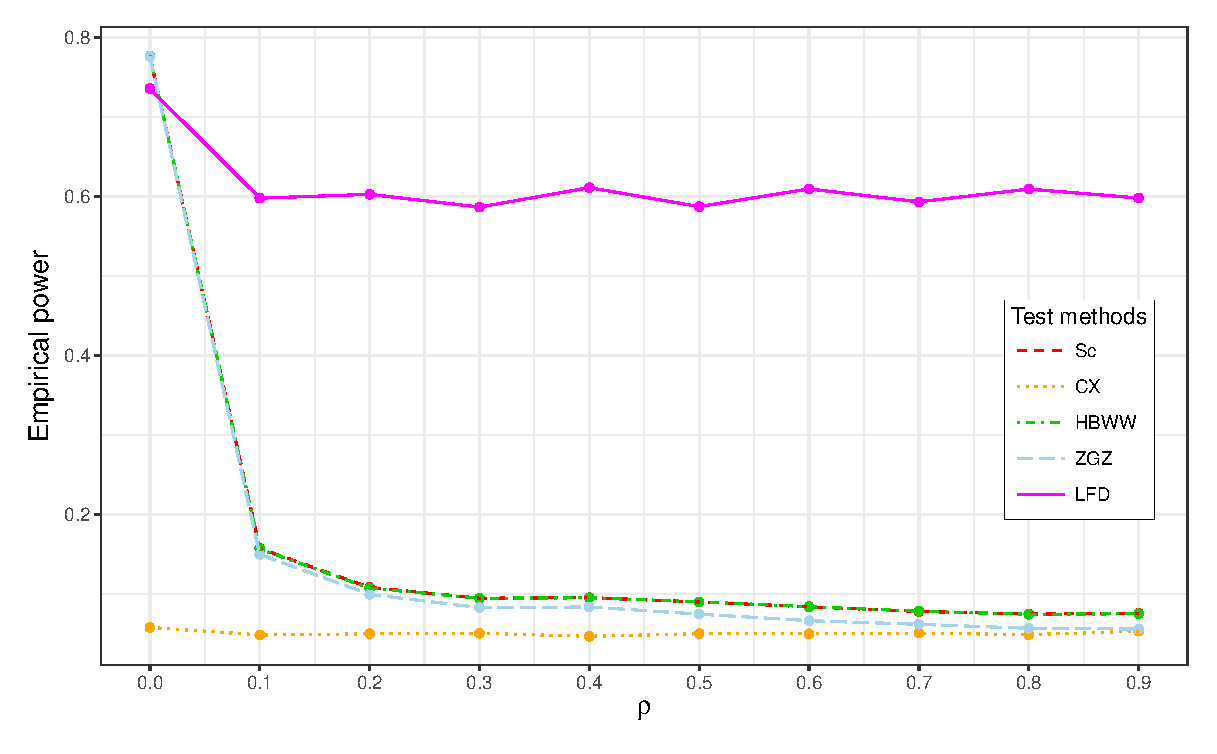
\includegraphics[width=12cm,height=12cm]{figure1}
    \caption{Empirical powers of tests. $\alpha=0.05$, $n_1=n_2=n_3=35$, $p=1000$.}\label{figure1}
\end{figure}





\section{Concluding remarks}\label{concluding}
In this paper, using the idea of least favorable direction, we proposed the LFD test for MANOVA in high dimensional setting.
We derived the asymptotic distribution of the LFD test statistic under both nonspiked and spiked covariances.
The asymptotic local power functions are also given.
From our theoretic results and simulation studies, it is seen that the LFD test has similar power behavior to existing tests when the covariance matrix is nonspiked, while tends to be much more powerful than existing tests when the covariance matrix is spiked.

For the case where the covariance structure is unknown,
we proposed an adaptive LFD test procedure by consistently detecting unknown covariance structure and estimating the unknown $r$.
However, this procedure relies on a hyperparameter $\tau$. 
How to choose an optimal $\tau$ is an interesting problem.
In addition, our proof relies on the normality of the observations.
It is unclear whether the same results hold without normal assumption.
We leave these topics for future research.



%Hence we use permutation method to determine the critical values throughout our simulations.
   %The test procedures resulting from permutation method have exact levels as long as the null distribution of observations are exchangeable~\citep{Romano1990On}.
   %The major down-side to permutation method is that it can be computationally intensive.
   %Fortunately, for LFD test statistic,  the permutation method has a simple implementation.
    %By expression~\eqref{statisticForm2}, a permuted statistic can be written as
    %\begin{equation}\label{permutedStatistic}
        %T(\bX\Gamma)=\lambda_{\max}\Big(\bC^\top{\big( \bJ^\top \Gamma^\top {(\bX^\top \bX)}^{-1} \Gamma \bJ \big)}^{-1}  \bC\Big),
    %\end{equation}
%where $\Gamma$ is an $n\times n$ permutation matrix.
   %Note that ${(\bX^\top \bX)}^{-1}$, the most time-consuming component, can be calculated aforehand.
   %The permutation procedure for LFD test statistic can be summarized as:
   %\begin{enumerate}
       %\item
           %Calculate $T(\bX)$ according to~\eqref{statisticForm2}, keep intermediate result ${(\bX^\top \bX)}^{-1}$.
       %\item For a large $M$, independently generate $M$ random permutation matrix $\Gamma_1,\ldots,\Gamma_M$ and calculate $T(\bX\Gamma_1),\ldots,T(\bX\Gamma_M)$ according to~\eqref{permutedStatistic}. 
       %\item Calculate the $p$-value by
           %$
           %\tilde{p}={(M+1)}^{-1}\big[1+\sum_{i=1}^M I\{T(\bX\Gamma_i)\geq T(\bX)\}\big]
           %$.
           %Reject the null hypothesis if $\tilde{p}\leq \alpha$.
   %\end{enumerate}
%
%Here $M$ is the permutation times. 
   %It can be seen that  step 1 and step 2 cost $O(n^2 p +n^3)$ and $O(n^2 M)$ operations respectively.
   %In large sample or high dimensional setting, step 2 has a negligible effect on total computational complexity.











%%%%%%%%%%%%%%%%%%%%%%%%%%%%%%%%%%%%%%%%%%%%%%%%%%%%%%%%%%%%%%%%%%%%%%%%%%%%%%%%%%%%%%%%%%%%%%%%%%%%%%%%%%%%%%%%%%%%%%%%%%%%
%\vskip 14pt
%\noindent {\large\bf Supplementary Materials}
%
%Contain
%the brief description of the online supplementary materials.
%\par
%%%%%%%%%%%%%%%%%%%%%%%%%%%%%%%%%%%%%%%%%%%%%%%%%%%%%%%%%%%%%%%%%%%%%%%%%%%%%%%%%%%%%%%%%%%%%%%%%%%%%%%%%%%%%%%%%%%%%%%%%%%%
\vskip 14pt
\noindent {\large\bf Acknowledgements}
This work was supported by the National Natural Science Foundation of
China under Grant Nos. 11471035, 11471030.
\par




\begin{appendices}
    \section{Technical details}\label{app}
\begin{lemma}\label{optProp}
    Suppose $\bA$ is a $p\times r$ matrix with rank $r$ and $\bB$ is a $p\times p$  non-zero positive semi-definite matrix.
    Denote by $\bA=\bU_\bA \bD_\bA \bV_\bA^\top$ the singular value decomposition of $\bA$, where $\bU_\bA$ and $\bV_\bA$ are $p\times r$ and $r\times r$ column orthogonal matrices, respectively, and $\bD_\bA$ is a $r\times r$ diagonal matrix.
    Let $\bP_\bA=\bU_\bA \bU_\bA^\top$ be the projection matrix onto the column space of $\bA$.
    Then
    \begin{equation}
        \max_{a^\top a=1, a^\top \bA \bA^\top a=0}a^\top \bB a=
        \lambda_{1}\big(\bB(\bI_p-\bP_\bA)\big).
    \end{equation}
\end{lemma}
\begin{proof}
    It can be seen that $a^\top \bA \bA^\top a=0$ if and only if $a= (\bI_p-\bP_\bA)a$.
    Then
    \begin{equation}\label{eq:prop1eq1}
        \begin{aligned}
        \max_{a^\top a=1, a^\top \bA \bA^\top a=0}a^\top \bB a
            &=
        \max_{a^\top a=1, \bP_\bA a=0}a^\top(\bI_p-\bP_\bA) \bB (\bI_p-\bP_\bA)a,
        \end{aligned}
    \end{equation}
    which is obviously no greater than $\lambda_1 \big((\bI-\bP_\bA)\bB(\bI-\bP_\bA)\big)$.
    To prove that they are equal,  without loss of generality, we can assume $\lambda_{1}\big((\bI-\bP_\bA)\bB(\bI-\bP_\bA)\big)>0$.
    Let $\alpha_1$ be one eigenvector corresponding to the largest eigenvalue of $(\bI-\bP_\bA)\bB(\bI-\bP_\bA)$.
    Since $(\bI-\bP_\bA)\bB(\bI-\bP_\bA)\bP_\bA=(\bI-\bP_\bA)\bB(\bP_\bA-\bP_\bA)=\bO_{p\times p}$ and $\bP_\bA$ is symmetric, the rows of $\bP_\bA$ are eigenvetors of $(\bI-\bP_\bA)\bB(\bI-\bP_\bA)$ corresponding to eigenvalue $0$.
    It follows that $\bP_\bA\alpha_1=0$.
    Therefore, $\alpha_1$ satisfies the constraint of~\eqref{eq:prop1eq1} and thus~\eqref{eq:prop1eq1} is no less than $\lambda_{1}\big((\bI-\bP_\bA)\bB(\bI-\bP_\bA)\big)$.
    The conclusion now follows by noting that $\lambda_{1}\big((\bI-\bP_\bA)\bB(\bI-\bP_\bA)\big)=\lambda_{1}\big( \bB(\bI-\bP_\bA)\big)$.
    
\end{proof}

\begin{lemma}
    Let $\xi_{n,i}$, $i=1,\ldots, n$, $n=1,2,\ldots$, be iid $s$-dimensional random vectors with mean zero, covariance matrix $\bM$ and finite fourth moment.
    For $n=1,2,\ldots$, let $\{a_{n,i}\}_{i=1}^n$ be real random variables which are independent of $\{\xi_{n,i}\}_{i=1}^n$ and satisfy 
    \begin{equation}\label{lycon}
        \frac{\max_{1\leq i\leq n}a_{n,i}^2}{\sum_{i=1}^n a_{n,i}^2}\xrightarrow{P}0.
    \end{equation}
    Then
    \begin{equation*}
    (\sum_{i=1}^n a_{n,i}^2)^{-1/2}\sum_{i=1}^n a_{n,i}\xi_{n,i} 
    \xrightarrow{\mathcal{L}}\mathcal{N}_s(0,\bM).
    \end{equation*}
    \label{CLTLEMMA}
\end{lemma}
\begin{proof}
    First we observe that if $\{a_{n,i}\}_{i=1}^n$ are fixed numbers satisfying~\eqref{lycon}, then Lyapunov central limit theorem and continuity theorem imply that 
    for any $t\in\mathbb{R}^s$,
    \begin{equation*}
        \myE\left[\exp\left(
    (\sum_{i=1}^n a_{n,i}^2)^{-1/2}\sum_{i=1}^n a_{n,i}it^\top \xi_{n,i} 
    \right)\right]
    \to
    \exp\left(-\frac{1}{2} t^\top \bM t\right).
    \end{equation*}

    We only need to prove that for every subsequence of $\{n\}$, there is a further subsequence along which the conclusion holds.
    Let $\{m(n)\}$  be a subsequence of $\{n\}$.
    We can find a further subsequence of $\{m(n)\}$ along which~\eqref{lycon} holds almost surely.
    Then along this subsequence, our previous argument implies that
    for any $t\in\mathbb{R}^s$,
    \begin{equation*}
        \myE
       \left[ 
        \exp\left(
    (\sum_{i=1}^n a_{n,i}^2)^{-1/2}\sum_{i=1}^n a_{n,i}it^\top \xi_{n,i} 
    \right)
    \bigg| a_{n,1},\ldots, a_{n,n}
\right]
    \to
    \exp\left(-\frac{1}{2} t^\top \bM t\right)
    \end{equation*}
    almost surely.
    Then by dominated convergence theorem,
    \begin{equation*}
        \myE
       \left[ 
        \exp\left(
    (\sum_{i=1}^n a_{n,i}^2)^{-1/2}\sum_{i=1}^n a_{n,i}it^\top \xi_{n,i} 
    \right)
\right]
    \to
    \exp\left(-\frac{1}{2} t^\top \bM t\right)
    \end{equation*}
    holds along this further subsequence. This implies the conclusion holds along this further subsequence, which completes the proof.




 
\end{proof}

    \begin{lemma}[Weyl's inequality]
        Let $\bA$ and $\bB$ be two symmetric $n\times n$ matrices. If $r+s-1\leq i \leq j+k-n$, we have
        $$
        \lambda_j(\bA) +\lambda_k(\bB)\leq \lambda_i (\bA+\bB) \leq
        \lambda_r(\bA)+\lambda_s(\bB).
        $$
        See, for example,~\citet{Horn1985Matrix} Theorem 4.3.1.
\end{lemma}
\begin{lemma}[von Neumann's trace theorem]
    Let $\bA$ and $\bB$ be two $m\times n$ matrices. Let $\sigma_1(\bA)\geq \ldots \geq \sigma_q (\bA)$ and $\sigma_1(\bB)\geq \cdots \geq \sigma_q (\bB)$ denote the non-increasingly ordered singular values of $\bA$ and $\bB$, respectively. Then
    \begin{equation*}
        \mytr(\bA \bB^\top)\leq \sum_{i=1}^{\min(m,n)}\sigma_i(\bA)\sigma_i(\bB).
    \end{equation*}
    See, for example,~\citet{Horn1985Matrix} Theorem 7.4.1.1.
\end{lemma}
%\begin{lemma}[\citet{DAVIDSON2001317} Theorem II.7]\label{DSbound}
    %Let $\bA$ be $m\times n$ random matrix with iid $\mathcal{N}(0,1)$ entries.
    %If $m>n$, then for any $t>0$,
    %\begin{align*}
        %\Pr(\sqrt{\lambda_1(\bA \bA^\top)}>\sqrt{m}+\sqrt{n}+t)\leq \exp(-t^2/2),\\
        %\Pr(\sqrt{\lambda_n(\bA \bA^\top)}<\sqrt{m}-\sqrt{n}-t)\leq \exp(-t^2/2).
    %\end{align*}
%\end{lemma}

\begin{lemma}\label{lemma:con}
    Let $\{Z_i\}_{i=1}^n$ be iid $m$-dimensional random vectors with common distribution $\mathcal{N}_m(\mathbf{0}_m,\bI_m)$.
    Then for any $n$-dimensional vector $\omega=(\omega_1,\ldots,\omega_n)^\top$, we have
\begin{equation*}
    \left\|\sum_{i=1}^n \omega_i(Z_i Z_i^\top - \bI_m)\right\|=O_P(|\omega|_2 \sqrt{m}+|\omega|_{\infty}m),
\end{equation*}
where $|\omega|_2=\sqrt{\sum_{i=1}^n \omega_i^2}$ and $|\omega|_{\infty}=\max_{1\leq i\leq n}|\omega_i|$.
\end{lemma}
\begin{remark}
    Our proof implies that the conclusion is still valid if $\omega$ is random and is independent of $\{Z_i\}_{i=1}^n$.
\end{remark}
\begin{proof}
    Our proof is adapted from the proof of Theorem 5.39 in~\cite{Vershynin2010Introduction}.
    By Lemma 5.2 and Lemma 5.4 of~\cite{Vershynin2010Introduction}, there exists a set $\mathcal{C}\subset \{x\in\mathbb{R}^m: |x|_2=1\}$ satisfying $\text{Card} (\mathcal{C})\leq 9^m$ such that for any $m\times m$ symmetric matrix $\bA$,
    \begin{equation}\label{eq:b1}
    \|A\|\leq 2\max_{x\in\mathcal{C}} x^\top \bA x.
\end{equation}
Then for $t>4$, 
\begin{equation*}
    \begin{split}
        &\Pr\left(
            \left\|\sum_{i=1}^n \omega_i(Z_i Z_i^\top - \bI_m)\right\|
            > t (|\omega|_2 \sqrt{m}+|\omega|_{\infty} m)
        \right)
        \\
        \leq &
        \Pr\left(
            2\sup_{x\in\mathcal{C}}\left|\sum_{i=1}^n \omega_i(x^\top Z_i Z_i^\top x - 1)\right|
            > t (|\omega|_2 \sqrt{m}+|\omega|_{\infty} m)
        \right)
        \\
        \leq &
        \sum_{x\in\mathcal{C}}
        \Pr\left(
            \left|\sum_{i=1}^n \omega_i(x^\top Z_i Z_i^\top x - 1)\right|
            >  2 |\omega|_2 \sqrt{\frac{mt}{4}}+2|\omega|_{\infty} \frac{mt}{4}
        \right)
        \\
        \leq & 2\cdot 9^{m} \exp\left(-\frac{mt}{4}\right)
        =2\exp\left((2\log 3 -t/4)m\right)
        ,
    \end{split}
\end{equation*}
where the first inequality follows from~\eqref{eq:b1}, the second inequality follows from the union bound and the third inequality follows Lemma 1 of~\cite{Laurent2000Adaptive}.
The upper bound $2\exp\left((2\log 3 -t/4)m\right)$ can be arbitrarily small as long as $t$ is large enough.
This completes the proof.
\end{proof}




\begin{proof}[\textbf{Proof of Proposition~\ref{eigenvalueProp}}]
    We only need to deal with the matrix $n^{-1}\bZ^\top \bLambda \bZ$ since it shares the same non-zero eigenvalues as $\hat{\bSigma}$.
    Write
    \begin{equation*}
        \begin{split}
        n^{-1}\bZ^\top \bLambda \bZ=&
        n^{-1}\bZ_1^\top \bLambda_1 \bZ_1+
        n^{-1}\bZ_2^\top \bLambda_2 \bZ_2
        \\
        =&
        n^{-1}\bZ_1^\top \bLambda_1 \bZ_1+
        n^{-1}\mytr(\bLambda_2)\bI_n+
        n^{-1}\left(\bZ_2^\top \bLambda_2 \bZ_2-\mytr(\bLambda_2)\bI_n\right)
        .
        \end{split}
    \end{equation*}
    Then Weyl's inequality implies that for $ i=1,\ldots, r$,
    \begin{equation}\label{eigenBoundForF}
        \begin{split}
        &
        \left|
        \lambda_i\left(n^{-1}\bZ^\top \bLambda \bZ\right)
        -
        \lambda_i(n^{-1}\bZ_1^\top \bLambda_1 \bZ_1)
        -
        n^{-1}
        \mytr(\bLambda_2)
        \right|
        \leq
        n^{-1}\left\|\bZ_2^\top \bLambda_2 \bZ_2-
        \mytr(\bLambda_2)
        \bI_n\right\|.
        \end{split}
    \end{equation}
    Using Weyl's inequality, we can derive the following lower bound for $\lambda_i(n^{-1}\bZ_1^\top \bLambda_1 \bZ_1)$, $ i=1,\ldots, r$.
\begin{equation*}\label{eq:DLower}
\begin{aligned}
\lambda_i(\bZ_1^\top \bLambda_1 \bZ_1)
\geq&
\lambda_i(\bZ_1^\top \mydiag(\blambda_i \bI_{i},\bO_{(r-i)\times(r-i)}) \bZ_1)
\\
    =&
    \lambda_i\Big( \blambda_i \bZ_1^\top \bZ_1-\blambda_i\bZ_1^\top \mydiag(\bO_{i\times i}, \bI_{r-i}) \bZ_1\Big)\\
    \geq&
    \lambda_r\Big( \blambda_i \bZ_1^\top \bZ_1\Big)+\lambda_{n+i-r}\Big(-\blambda_i\bZ_1^\top \mydiag(\bO_{i\times i}, \bI_{r-i}) \bZ_1\Big)\\
= &
\blambda_i \lambda_r(\bZ_1\bZ_1^\top).
\end{aligned}
\end{equation*}
Similarly, we can derive the following upper bound for
$\lambda_i(\bZ_1^\top \bLambda_1 \bZ_1)$, $i=1,\ldots,r$.
\begin{equation*}\label{eq:DUpper}
\begin{aligned}
&\lambda_i(\bZ_1^\top \bLambda_1 \bZ_1)
\\
=&\lambda_i\Big(
\bZ_1^\top \big(
\mydiag(\blambda_1,\ldots,\blambda_{i-1},\bO_{(r-i+1)\times(r-i+1)})+
\mydiag(\bO_{(i-1)\times(i-1)},\blambda_i,\ldots,\blambda_r)
\big)
\bZ_1
\Big)\\
\leq&\lambda_i\Big(
\bZ_1^\top \big(
\mydiag(\blambda_1,\ldots,\blambda_{i-1},\bO_{(r-i+1)\times(r-i+1)})
\Big)
+
\lambda_1\Big(
\mydiag(\bO_{(i-1)\times(i-1)},\blambda_i,\ldots,\blambda_r)
\big)
\bZ_1
\Big)\\
%\leq&
%\lambda_1(\bZ_{1[1:r,:]}^\top \mydiag(\bO_{(i-1)\times(i-1)},\lambda_i,\ldots,\lambda_r) \bZ_{1[1:r,:]})
    \leq&
\lambda_1(\bZ_1^\top \mydiag(\bO_{(i-1)\times(i-1)},\blambda_i \bI_{r-i+1}) \bZ_1)
\leq  \blambda_i \lambda_1(\bZ_1\bZ_1^\top).
\end{aligned}
\end{equation*}
The above lower bound and upper bound imply
\begin{equation}\label{eigenBoundForA}
    \begin{aligned}
\left|
\lambda_i(n^{-1}\bZ_1^\top \bLambda_1 \bZ_1)-\blambda_i
\right|
\leq&
\blambda_i 
\max\left(
    |\lambda_1(n^{-1}\bZ_1 \bZ_1^\top)-1|,
    |\lambda_r(n^{-1}\bZ_1 \bZ_1^\top)-1|
\right)
\\
=&\blambda_i \|n^{-1}\bZ_1\bZ_1^\top -\bI_r\|.
    \end{aligned}
\end{equation}
Combining the bounds~\eqref{eigenBoundForF} and~\eqref{eigenBoundForA} gives that for $i=1,\ldots,r$,
\begin{equation*}
    \begin{split}
        &
        \left|
        \lambda_i\left(n^{-1}\bZ^\top \bLambda \bZ\right)
        -
        \blambda_i
        -
        n^{-1}\mytr(\bLambda_2)
        \right|
        \\
        \leq&
        n^{-1}\left\|\bZ_2^\top \bLambda_2 \bZ_2-\mytr(\bLambda_2) \bI_n\right\|
        +\blambda_i \|n^{-1}\bZ_1\bZ_1^\top -\bI_r\|.
    \end{split}
\end{equation*}
From Lemma~\ref{lemma:con}, we have
\begin{align}
    \label{conB2B1}
            \|n^{-1}\bZ_1\bZ_1^\top -\bI_r\|&=
            O_P\left(\sqrt{\frac{r}{n}}\right),
        \\
        \label{conB2B}
        n^{-1}\left\|\bZ_2^\top \bLambda_2 \bZ_2-\mytr(\bLambda_2)\bI_n\right\|&=O_P\left(\sqrt{\frac{\mytr(\bLambda_2^2)}{ n}}+\blambda_{r+1}\right).
\end{align}
This proves the first statement.

Next we prove the second statement. Note that
\begin{equation*}
    \begin{split}
     \sum_{i=r+1}^n\lambda_i(\hat{\bSigma})
    =&
    \sum_{i=r+1}^n\lambda_i(n^{-1}\ \bZ^\top \bLambda \bZ)
    \\
    =&
    \mytr (n^{-1}\bZ^\top \bLambda \bZ) -\sum_{i=1}^r\lambda_i(n^{-1}\ \bZ^\top \bLambda \bZ)
    \\
    =&
    \mytr (n^{-1}\bZ_2^\top \bLambda_2 \bZ_2)
    -\frac{r}{n} \mytr(\bLambda_2)
    \\
    &-
    \left(
    \sum_{i=1}^r\lambda_i(n^{-1}\ \bZ^\top \bLambda \bZ)
    -
    \mytr (n^{-1}\bZ_1^\top \bLambda_1 \bZ_1)
    -\frac{r}{n} \mytr(\bLambda_2)
\right)
    .
    \end{split}
\end{equation*}
It follows from inequalities~\eqref{eigenBoundForF} and~\eqref{conB2B} that
\begin{equation*}
    \begin{split}
    &\left|
    \sum_{i=1}^r\lambda_i(n^{-1}\ \bZ^\top \bLambda \bZ)
    -\mytr (n^{-1}\bZ_1^\top \bLambda_1 \bZ_1)- 
    \frac{r}{n}\mytr(\bLambda_2)
    \right|
    \\
    \leq & \frac{r}{n}
    \left\|\bZ_2^\top \bLambda_2 \bZ_2-\mytr(\bLambda_2)\bI_n\right\|
    =
    O_P\left(
    r\sqrt{\frac{\mytr(\bLambda_2^2)}{ n}}+r\blambda_{r+1}
    \right)
    .
    \end{split}
\end{equation*}
Thus,
\begin{equation*}
        \sum_{i=r+1}^n\lambda_i(\hat{\bSigma})
    =
    \mytr (n^{-1}\bZ_2^\top \bLambda_2 \bZ_2)
    -
    \frac{r}{n}\mytr(\bLambda_2)
    +O_P\left(
    r\sqrt{\frac{\mytr(\bLambda_2^2)}{ n}}+r\blambda_{r+1}
    \right)
    .
\end{equation*}
It is straightforward to show that
\begin{equation*}
    \myE \mytr (n^{-1}\bZ_2^\top \bLambda_2 \bZ_2)=\mytr(\bLambda_2),
    \quad
    \myVar \left(\mytr (n^{-1}\bZ_2^\top \bLambda_2 \bZ_2)\right)
    =\frac{2}{n}\mytr(\bLambda_2^2).
\end{equation*}
Hence
\begin{equation*}
    \begin{split}
     &\sum_{i=r+1}^n\lambda_i(\hat \bSigma)
     \\
    =&
\mytr(\bLambda_2)+O_P\left(\sqrt{\frac{\mytr(\bLambda_2^2)}{ n}}\right)
    -
    \frac{r}{n}\mytr(\bLambda_2)
    +O_P\left(
    r\sqrt{\frac{\mytr(\bLambda_2^2)}{ n}}+r\blambda_{r+1}
\right)
     \\
    =&
\mytr(\bLambda_2)
    -
    \frac{r}{n}\mytr(\bLambda_2)
    +O_P\left(
    r\sqrt{\frac{\mytr(\bLambda_2^2)}{ n}}+r\blambda_{r+1}
\right)
    .
    \end{split}
\end{equation*}
This completes the proof of the second statement.
\end{proof}

\begin{proof}[\textbf{Proof of Proposition~\ref{eigenvalueProp:R3}}]
    The first two statements are direct consequences of Proposition~\ref{eigenvalueProp} and the condition $r=o(n)$.
    Next we prove the third statement.
    We have
        $
        \widehat{\mytr(\bLambda_2^2)}
        =
        n^{-2}\sum_{i=r+1}^n \lambda_i^2(\bY^\top \bY-\widehat{\mytr(\bLambda_2)}\bI_n)
        $.
        Note that Weyl's inequality implies that for $i=r+1,\ldots,n$,
        \begin{equation*}
            \lambda_{i}(\bZ_2^\top \bLambda_2 \bZ_2 - \widehat{\mytr(\bLambda_2)}\bI_n)
            \leq
            \lambda_i(\bY^\top \bY-\widehat{\mytr(\bLambda_2)}\bI_n)
            \leq
            \lambda_{i-r}(\bZ_2^\top \bLambda_2 \bZ_2 - \widehat{\mytr(\bLambda_2)}\bI_n).
        \end{equation*}
Define
\begin{align*}
&\mathcal{C}_1=
\left\{i:
    1\leq i\leq n,\, \lambda_i\left(\bZ_2^\top \bLambda_2 \bZ_2-\widehat{\mytr(\bLambda_2)}\bI_n\right)> 0
\right\},
\\
&\mathcal{C}_2=
\left\{i:
    r+1\leq i\leq n, \,
    \lambda_{i-r}\left(\bZ_2^\top \bLambda_2 \bZ_2-\widehat{\mytr(\bLambda_2)}\bI_n\right)\leq 0
\right\}.
\end{align*}
It can be seen that $\mathcal{C}_1\cap \mathcal{C}_2 =\emptyset$ and $\text{Card}(\mathcal{C}_1\cup\mathcal{C}_2)= n - r$.
For $i\geq r+1$ and $i\in \mathcal{C}_1$,
    \begin{equation*}
        \lambda_i^2(\bZ_2^\top \bLambda_2 \bZ_2-\widehat{\mytr(\bLambda_2)}\bI_n) \leq \lambda_i^2(\bY^\top \bY-\widehat{\mytr(\bLambda_2)}\bI_n)\leq \lambda_{i-r}^2(\bZ_2^\top \bLambda_2 \bZ_2-\widehat{\mytr(\bLambda_2)}\bI_n);
    \end{equation*}
for $i\in \mathcal{C}_2$,
    \begin{equation*}
        \lambda_{i-r}^2(\bZ_2^\top \bLambda_2 \bZ_2-\widehat{\mytr(\bLambda_2)}\bI_n) \leq \lambda_i^2(\bY^\top \bY-\widehat{\mytr(\bLambda_2)}\bI_n)\leq \lambda_{i}^2(\bZ_2^\top \bLambda_2 \bZ_2-\widehat{\mytr(\bLambda_2)}\bI_n);
    \end{equation*}
    for $i\geq r+1$ and $i\notin \mathcal{C}_1\cup \mathcal{C}_2$,
    \begin{equation*}
        \lambda_i^2(\bY^\top \bY-\widehat{\mytr(\bLambda_2)}\bI_n)\leq
        \max
        \left(
            \lambda_{i-r}^2(\bZ_2^\top \bLambda_2 \bZ_2-\widehat{\mytr(\bLambda_2)}\bI_n) 
        ,
        \lambda_{i}^2(\bZ_2^\top \bLambda_2 \bZ_2-\widehat{\mytr(\bLambda_2)}\bI_n)
    \right).
    \end{equation*}
    Therefore,
    \begin{equation}\label{abcd0}
        \begin{split}
            &\left|
            \sum_{i=r+1}^n \lambda_i^2\left(\bY^\top \bY-\widehat{\mytr(\bLambda_2)}\bI_n\right)
            -\mytr(\bZ_2^\top \bLambda_2 \bZ_2-\widehat{\mytr(\bLambda_2)}\bI_n)^2
            \right|
            \\
            \leq&
            \left|
            \sum_{i>r,\, i\in \mathcal{C}_1} \lambda_i^2\left(\bY^\top \bY-\widehat{\mytr(\bLambda_2)}\bI_n\right)
            -\sum_{i\in\mathcal{C}_1}\lambda_i^2\left(\bZ_2^\top \bLambda_2 \bZ_2-\widehat{\mytr(\bLambda_2)}\bI_n\right)
            \right|
            \\
            &+
            \left|
            \sum_{i>r,\, i\in \mathcal{C}_2} \lambda_i^2\left(\bY^\top \bY-\widehat{\mytr(\bLambda_2)}\bI_n\right)
            -\sum_{i\notin \mathcal{C}_1}\lambda_i^2\left(\bZ_2^\top \bLambda_2 \bZ_2-\widehat{\mytr(\bLambda_2)}\bI_n\right)
            \right|
            \\
            &+
            \left|
            \sum_{i>r,\, i\notin \mathcal{C}_1\cup\mathcal{C}_2} \lambda_i^2\left(\bY^\top \bY-\widehat{\mytr(\bLambda_2)}\bI_n\right)
            \right|
            \\
            \leq & 3r \|\bZ_2^\top \bLambda_2 \bZ_2-\widehat{\mytr(\bLambda_2)}\bI_n\|^2\\
            \leq & 3r \left(\|\bZ_2^\top \bLambda_2 \bZ_2-\mytr(\bLambda_2)\bI_n\|+\left|\mytr(\bLambda_2)-\widehat{\mytr(\bLambda_2)}\right|\right)^2\\
            = & 
            O_P\left(rn \mytr(\bLambda_2^2) + r n^2 \blambda_{r+1}^2\right)
            .
        \end{split}
    \end{equation}
    where the last equality follows from~\eqref{conB2B} and the first statement of the proposition.

    Now we deal with $\mytr(\bZ_2^\top \bLambda_2 \bZ_2-\widehat{\mytr(\bLambda_2)}\bI_n)^2$.
    Let $Z_{2,i}$ be the $i$th column of $\bZ_2$, $i=1,\ldots, n$.
    Then
    \begin{equation*}
        \mytr(\bZ_2^\top \bLambda_2 \bZ_2-\widehat{\mytr(\bLambda_2)}\bI_n)^2
        =
        \sum_{i=1}^n (Z_{2,i}^\top \bLambda_2 Z_{2,i}-\widehat{\mytr(\bLambda_2)})^2
        +
        2\sum_{1\leq i<j\leq n} (Z_{2,i}^\top \bLambda_2 Z_{2,j})^2.
    \end{equation*}
    For the first term, we have 
    \begin{equation*}
        \sum_{i=1}^n (Z_{2,i}^\top \bLambda_2 Z_{2,i}-\widehat{\mytr(\bLambda_2)})^2
        \leq
        2\sum_{i=1}^n (Z_{2,i}^\top \bLambda_2 Z_{2,i}-\mytr(\bLambda_2))^2
        +2n(\widehat{\mytr(\bLambda_2)}-\mytr(\bLambda_2))^2.
    \end{equation*}
    Then it follows from the first statement of the proposition and the fact $
        \myE
        \sum_{i=1}^n (Z_{2,i}^\top \bLambda_2 Z_{2,i}-\mytr(\bLambda_2))^2
        =2n \mytr(\bLambda_2^2)
        $ that
        \begin{equation}\label{abcd1}
        \sum_{i=1}^n (Z_{2,i}^\top \bLambda_2 Z_{2,i}-\widehat{\mytr(\bLambda_2)})^2
        =O_P\left((n+r^2)\mytr(\bLambda_2^2)+r^2 n \blambda_{r+1}^2\right).
\end{equation}
    For the second term, it is straightforward to show that
    $\myE 2\sum_{1\leq i<j\leq n} (Z_{2,i}^\top \bLambda_2 Z_{2,j})^2=n(n-1)\mytr(\bLambda_2^2)$.
    Furthermore, \cite{chen2010tests}, Proposition A.2 implies that
    \begin{equation*}
        \begin{split}
        \myVar\left(
            2\sum_{1\leq i<j\leq n} (Z_{2,i}^\top \bLambda_2 Z_{2,j})^2
        \right)
        =& O\left(
            n^2 \mytr^2 (\bLambda_2^2) + n^3 \mytr(\bLambda_2^4)
        \right)
        \\
        =& O\left(
            n^2 \mytr^2 (\bLambda_2^2) + n \mytr(\bLambda_{2}^2) n^2 \blambda_{r+1}^2
        \right)
        \\
        =& O\left(
            n^2 \mytr^2 (\bLambda_2^2) + n^4 \blambda_{r+1}^4
        \right)
        .
        \end{split}
    \end{equation*}
    Thus,
    \begin{equation*}
            2\sum_{1\leq i<j\leq n} (Z_{2,i}^\top \bLambda_2 Z_{2,j})^2
            =
            n^2 \mytr(\bLambda_2^2)+O_P\left( n \mytr(\bLambda_2^2)+ n^{2}\blambda_{r+1}^2\right).
    \end{equation*}
    Combining the last display and~\eqref{abcd1} yields
    \begin{equation*}
        \mytr(\bZ_2^\top\bLambda_2 \bZ_2-\widehat{\mytr(\bLambda_2)}\bI_n)^2
        =
        n^2 \mytr(\bLambda_2^2)+O_P\left( (n+r^2) \mytr(\bLambda_2^2)+ (n+r^2)n\blambda_{r+1}^2\right)
        .
    \end{equation*}
    Combine the last display and~\eqref{abcd0}, we have
    \begin{equation*}
            \sum_{i=r+1}^n \lambda_i^2\left(\bY^\top \bY-\widehat{\mytr(\bLambda_2)}\bI_n\right)
            =
            O_P\left(rn \mytr(\bLambda_2^2) + r n^2 \blambda_{r+1}^2\right).
    \end{equation*}
    This completes the proof.

\end{proof}



\begin{proposition}\label{newEigenvectorProp}
    Suppose that $r=o(n)$ and $r\blambda_{r+1} /\mytr(\bLambda_2)\to 0$. Then
    \begin{equation*}
        \|\bP_{\bY,1} -\bP_{\bY,1}^* \|
        =O_P\left(\frac{\blambda_{r+1}+n^{-1}\mytr(\bLambda_2)}{\blambda_r +n^{-1}\mytr(\bLambda_2)}\right),
    \end{equation*}
    where
    \begin{equation*}
        \bP_{\bY,1}^*=
    \bU
    \begin{pmatrix}
       \bI_r \\
       \bQ
    \end{pmatrix}
    \left(\bI_r+ \bQ^\top \bQ \right)^{-1}
    \begin{pmatrix}
        \bI_r
          &
          \bQ^\top
        \end{pmatrix}
        \bU^\top.
    \end{equation*}
\end{proposition}
\begin{proof}
    The following intermediate matrix
    \begin{equation*}
        \begin{split}
    \hat{\bSigma}_0 =&
    n^{-1}\bU_1 \bLambda_1^{1/2} \bZ_1 \bZ_1^\top \bLambda_1^{1/2}\bU_1^\top
    +n^{-1}\bU_1 \bLambda_1^{1/2} \bZ_1 \bZ_2^\top \bLambda_2^{1/2}\bU_2^\top
    +n^{-1}\bU_2 \bLambda_2^{1/2} \bZ_2 \bZ_1^\top \bLambda_1^{1/2}\bU_1^\top
    \\
    &+n^{-1}\bU_2 \bLambda_2^{1/2} \bZ_2 \bV_{\bZ_1}\bV_{\bZ_1}^\top
    \bZ_2^\top \bLambda_2^{1/2}\bU_2^\top
        \end{split}
    \end{equation*}
    plays a key role in the proof.
    It can be seen that 
    \begin{equation*}
        \hat{\bSigma}_0=n^{-1}
    \bU
    \begin{pmatrix}
       \bI_r \\
       \bQ
    \end{pmatrix}
    \bLambda_1^{1/2}\bZ_1 \bZ_1^\top\bLambda_1^{1/2}
    \begin{pmatrix}
        \bI_r
          &
          \bQ^\top
        \end{pmatrix}
        \bU^\top.
    \end{equation*}
    Consequently, $\hat{\bSigma}_0$ is a positive semi-definite matrix with rank $r$, and $\bP_{\bY,1}^*$ is the projection matrix onto the rank $r$ principal subspace of $\hat{\bSigma}_0$.

    From~\cite{Cai2015Optimal}, Proposition 1, we have
    \begin{equation}\label{asd1}
        \|\bP_{\bY,1} -\bP_{\bY,1}^* \|
        \leq 
        \frac{2\|\hat{\bSigma}-\hat{\bSigma}_0\|}{\lambda_r(\hat{\bSigma}_0)}.
    \end{equation}
    We have the following upper bound for $\|\hat{\bSigma}-\hat{\bSigma}_0\|$.
    \begin{equation}\label{asd2}
        \begin{split}
            \|\hat{\bSigma}-\hat{\bSigma}_0\|
            =&
    n^{-1}\left\|\bU_2 \bLambda_2^{1/2} \bZ_2  
    \bZ_2^\top \bLambda_2^{1/2}\bU_2^\top
    -\bU_2 \bLambda_2^{1/2} \bZ_2 
    \bV_{\bZ_1}
    \bV_{\bZ_1}^\top
    \bZ_2^\top \bLambda_2^{1/2}\bU_2^\top
    \right\|
    \\
     =&
    n^{-1}\left\|
     \bLambda_2^{1/2} \bZ_2 
    (\bI_n-\bV_{\bZ_1}
    \bV_{\bZ_1}^\top)
    \bZ_2^\top \bLambda_2^{1/2}
    \right\|
    \\
    \leq &
    n^{-1}\left\|\bZ_2^\top \bLambda_2 \bZ_2\right\|
    \\
 \leq& 
     n^{-1}\left\| \bZ_2^\top \bLambda_2\bZ_2-\mytr(\bLambda_2)\bI_n\right\|
     +n^{-1}
     \mytr(\bLambda_2)
     \\
     =&O_P\left( 
\sqrt{\frac{\mytr\left(\bLambda_2^2\right)}{n}}+\blambda_{r+1}
     +
     n^{-1}\mytr(\bLambda_2)
 \right)
 \\
     =&O_P\left( 
\blambda_{r+1}
     +
     n^{-1}\mytr(\bLambda_2)
 \right)
 ,
    \end{split}
\end{equation}
where
the second last equality follows from~\eqref{conB2B} and the last equality follows from
\begin{equation*}
    \sqrt{\frac{\mytr\left(\bLambda_2^2\right)}{n}}
    \leq
    \sqrt{\frac{\blambda_{r+1}\mytr\left(\bLambda_2\right)}{n}}
    \leq
    \frac{1}{2}\left(\blambda_{r+1}+n^{-1}\mytr\left(\bLambda_2\right)\right).
\end{equation*}
Now we deal with $\lambda_r(\hat{\bSigma}_0)$.
We have
\begin{equation*}
    \begin{split}
     \lambda_r(\hat{\bSigma}_0)
     =&\lambda_r\left(
n^{-1}
  (\bZ_1\bZ_1^\top)^{1/2}\bLambda_1^{1/2}(\bI_r +\bQ^\top \bQ)\bLambda_1^{1/2} (\bZ_1\bZ_1^\top)^{1/2}
     \right)
     \\
     =&
     \lambda_r\left(
        n^{-1} (\bZ_1\bZ_1^\top)^{1/2}
         \bLambda_1 
         (\bZ_1\bZ_1^\top)^{1/2}
         +
         n^{-1} \bV_{\bZ_1}^\top \bZ_2^\top \bLambda_2 \bZ_2 \bV_{\bZ_1} 
    \right).
    \end{split}
\end{equation*}
It can be seen that $\bZ_2 \bV_{\bZ_1}$ is a $(p-r)\times r$ random matrix with iid $\mathcal{N}(0,1)$ entries.
Then Lemma~\ref{lemma:con} implies that
\begin{equation}\label{projCon}
        \begin{split}
        \left\|n^{-1}  \bV_{\bZ_1}^\top \bZ_2^\top \bLambda_2 \bZ_2 \bV_{\bZ_1} 
        -n^{-1} \mytr(\bLambda_2) \bI_r
        \right\|
        =&
        O_P\left(
            n^{-1}\sqrt{r\mytr\left(\bLambda_2^2\right)}
            +rn^{-1}\blambda_{r+1}
        \right)
        \\
        =&
        O_P\left(
            n^{-1}\sqrt{r\blambda_{r+1}\mytr\left(\bLambda_2\right)}
            +rn^{-1}\blambda_{r+1}
        \right)
        \\
        =&o_P\left(n^{-1}\mytr(\bLambda_2)\right)
        ,
        \end{split}
    \end{equation}
    where the last equality follows from the condition $r\blambda_{r+1} /\mytr(\bLambda_2)\to 0$.
    Then it follows from Weyl's inequality that 
    \begin{equation*}
        \begin{split}
        &\left| 
        \lambda_r (\hat{\bSigma}_0)-
     \lambda_r\left(
        n^{-1} (\bZ_1\bZ_1^\top)^{1/2}
         \bLambda_1 
         (\bZ_1\bZ_1^\top)^{1/2}
         +
         n^{-1} \mytr(\bLambda_2)\bI_r 
    \right)
    \right|
\\
\leq &\left\|n^{-1} \bV_{\bZ_1}^\top \bZ_2^\top \bLambda_2 \bZ_2 \bV_{\bZ_1} 
        -n^{-1} \mytr(\bLambda_2) \bI_r
        \right\|
        \\
        =&o_P\left(n^{-1}\mytr(\bLambda_2)\right).
        \end{split}
    \end{equation*}
    On the other hand,~\eqref{eigenBoundForA} and~\eqref{conB2B1} imply that
    \begin{equation*}
        \begin{split}
        &
     \lambda_r\left(
        n^{-1} (\bZ_1\bZ_1^\top)^{1/2}
         \bLambda_1 
         (\bZ_1\bZ_1^\top)^{1/2}
         +
         n^{-1} \mytr(\bLambda_2)\bI_r 
    \right)
\\
        =&
     \lambda_r\left(
        n^{-1} \bZ_1^\top
         \bLambda_1 
         \bZ_1
    \right)
         +
         n^{-1} \mytr(\bLambda_2)
        \\
        =&
        \blambda_r +o_P(\blambda_r)
         +
         n^{-1} \mytr(\bLambda_2).
        \end{split}
    \end{equation*}
    Hence we have 
    \begin{equation}\label{asd3}
    \lambda_r(\hat{\bSigma}_0)=(1+o_P(1))(\blambda_r+n^{-1}\mytr(\bLambda_2)).
    \end{equation}
    Then the conclusion follows from~\eqref{asd1},~\eqref{asd2} and~\eqref{asd3}.
\end{proof}

\begin{proof}[\textbf{Proof of Proposition~\ref{newEigenvectorPropCor}}]
    Note that
    \begin{equation*}
        \begin{split}
        &
        \left\|
\bP_{\bY,1}
         - 
\bP_{\bY,1}^{\dagger}
        \right\|
        \leq
        \left\|
\bP_{\bY,1}
-
        \bP_{\bY,1}^*
        \right\|
        +
        \left\|
        \bP_{\bY,1}^* 
            -
\bP_{\bY,1}^{\dagger}
            \right\|.
        \end{split}
    \end{equation*}
    Under the condition $\mytr(\bLambda_2)/(n\blambda_r)\to 0$, Proposition~\ref{newEigenvectorProp} implies that
    \begin{equation*}
        \left\|
\bP_{\bY,1}-
        \bP_{\bY,1}^*
        \right\|
    =O_P\left(\frac{\blambda_{r+1}}{\blambda_r}+\frac{\mytr(\bLambda_2)}{n\blambda_r}\right).
    \end{equation*}
    So we only need to deal with $
        \|
        \bP_{\bY,1}^* 
            -
\bP_{\bY,1}^{\dagger}
            \|
    $.
    We have
    \begin{equation*}
        \begin{split}
        &\left\|
        \bP_{\bY,1}^* 
            -
\bP_{\bY,1}^{\dagger}
        \right\|
        \\
        \leq&
        \Big\|
        \bP_{\bY,1}^* 
        -
        \bU
        \begin{pmatrix}
           \bI_r \\
           \bQ
        \end{pmatrix}
        \begin{pmatrix}
            \bI_r
              &
              \bQ^\top
            \end{pmatrix}
            \bU^\top
        \Big\|
        +
        \Big\|
        \bU
        \begin{pmatrix}
           \bI_r \\
           \bQ
        \end{pmatrix}
        \begin{pmatrix}
            \bI_r
              &
              \bQ^\top
            \end{pmatrix}
            \bU^\top
            -
\bP_{\bY,1}^{\dagger}
        \Big\|
        \\
        =&
        \Big\|
        \begin{pmatrix}
           \bI_r \\
           \bQ
        \end{pmatrix}
        \left(
            \left(\bI_r+\bQ^{\top}\bQ \right)^{-1}
            -\bI_r
        \right)
        \begin{pmatrix}
            \bI_r
              &
              \bQ^\top
            \end{pmatrix}
        \Big\|
        +\left\| \bU_2 \bQ \bQ^\top \bU_2^\top \right\|
        \\
        =&
        \Big\|
        \left(
            \left(\bI_r+\bQ^{\top}\bQ \right)^{-1}
            -\bI_r
        \right)
        \left(\bI_r + \bQ^\top \bQ \right)
        \Big\|
        +\left\| \bU_2 \bQ \bQ^\top \bU_2^\top \right\|
        \\
        =&2 \left\| \bQ^\top \bQ\right\|
        .
        \end{split}
    \end{equation*}
    Note that
    \begin{equation}\label{UpperBoundQ}
        \begin{split}
        \|\bQ^\top \bQ \|
        =& \left\|
        \bLambda_1^{-1/2} (\bZ_1 \bZ_1^\top)^{-1/2} \bV_{\bZ_1}^\top \bZ_2^\top \bLambda_2 \bZ_2 \bV_{\bZ_1} (\bZ_1 \bZ_1^\top)^{-1/2} \bLambda_1^{-1/2}
        \right\|
        \\
        \leq &
        \blambda_r^{-1}\left\|(\bZ_1\bZ_1^\top)^{-1}\right\| \left\|\bV_{\bZ_1}^\top \bZ_2^\top \bLambda_2 \bZ_2 \bV_{\bZ_1}\right\|
        \\
= & O_P\left(\frac{\mytr(\bLambda_2)}{n\blambda_r}\right),
        \end{split}
    \end{equation}
    where the second last equality follows from the fact $\|(\bZ_1 \bZ_1^\top)^{-1}\|=\lambda_r(\bZ_1\bZ_1^\top)^{-1}$, \eqref{conB2B1},~\eqref{projCon} and Weyl's inequality.
    Therefore, we have 
    \begin{equation*}
        \left\|
        \bP_{\bY,1}^* 
            -
\bP_{\bY,1}^{\dagger}
            \right\|= O_P\left(\frac{\mytr(\bLambda_2)}{n\blambda_r}\right)
            .
    \end{equation*}
    This completes the proof.

\end{proof}


\begin{proposition}
    \label{eigenvectorprop2}
    Suppose that $r=o(n)$ and $n\blambda_{r+1} /\mytr(\bLambda_2)\to 0$. Then
    \begin{equation*}
            \left\|
            \bP_{\bY,2}
            -
            \bP_{\bY,2}^*
            \right\|
    = 
    O_P\left(
        \min\left(
        \sqrt{\frac{\mytr(\bLambda_2) \blambda_1}{n\blambda_r^2}}
    ,1\right)
    \right)
    .
    \end{equation*}
where
$
            \bP_{\bY,2}^*=
            \bU_2 \bLambda_2^{1/2}\bZ_{2} \tilde{\bV}_{\bZ_1}
            \left(\tilde{\bV}_{\bZ_1}^\top \bZ_2^\top \bLambda_2 \bZ_2 \tilde{\bV}_{\bZ_1}\right)^{-1}
            \tilde{\bV}_{\bZ_1}^\top \bZ_2^\top \bLambda_2^{1/2} \bU_2^\top
            $.
\end{proposition}
%\begin{remark}
    %The condition $n\blambda_{r+1} /\mytr(\bLambda_2)\to 0$ implies $n/\myrank(\bLambda_2) \to 0$.
    %Consequently, the matrix $\tilde{\bV}_{\bZ_1}^\top \bZ_2^\top \bLambda_2 \bZ_2 \tilde{\bV}_{\bZ_1}$ is invertible with probability $1$ for large $n$.
%\end{remark}
\begin{proof}
    We only need to prove that for any subsequence of $\{n\}$, there is a further subsequence along which the conclusion holds.
    Thus, without loss of generality, we assume $\mytr(\bLambda_2)\blambda_1 /{(n \blambda_r^2)}\to c\in [0,+\infty]$.
    Since $
    \bP_{\bY,2}
    $ and 
    $
    \bP_{\bY,2}^*
            $
            are both projection matrices, we have
            $
            \left\|
    \bP_{\bY,2}
    -
            \bP_{\bY,2}^*
            \right\|
            \leq 2
            $
    .
    Therefore, the conclusion holds if $c>0$.
    In the rest of the proof, we assume $c=0$, that is $\mytr(\bLambda_2)\blambda_1 /{(n \blambda_r^2)}\to 0$.


    Note that $\bU_{\bY,2}$ is in fact the leading $n-r$ eigenvectors of $(\bI_p -\bP_{\bY,1})\hat{\bSigma}(\bI_p -\bP_{\bY,1})$.
    Under the condition $n\blambda_{r+1}/\mytr(\bLambda_2)\to 0$,
    Proposition~\ref{newEigenvectorPropCor} implies that 
    \begin{equation*}
        \left\|
        \bP_{\bY,1}
        - 
\bP^\dagger_{\bY,1}
        \right\|
    =O_P\left(\frac{\mytr(\bLambda_2)}{n\blambda_r}\right).
    \end{equation*}
    It can be seen that
    \begin{equation*}
        \begin{split}
             &
             \left\|(\bI_p -\bP_{\bY,1})\hat{\bSigma}(\bI_p -\bP_{\bY,1})
             -
             (\bI_p -\bP^\dagger_{\bY,1})\hat{\bSigma}(\bI_p-\bP^\dagger_{\bY,1})
             \right\|
             \\
             \leq&
             \left\|
             (\bP^\dagger_{\bY,1}-\bP_{\bY,1})\hat{\bSigma}(\bP^\dagger_{\bY,1}-\bP_{\bY,1})
             \right\|
             +
             2\left\|
             (\bP^\dagger_{\bY,1}-\bP_{\bY,1})\hat{\bSigma}(\bI_p-\bP^\dagger_{\bY,1})
             \right\|
             .
        \end{split}
    \end{equation*}
    Under the condition $n\blambda_{r+1}/\mytr(\bLambda_2)\to 0$, Proposition~\ref{eigenvalueProp} implies that
    \begin{equation*}
        \|\hat{\bSigma}\|
        =\blambda_1\left(
            1+\frac{\mytr(\bLambda_2)}{n\blambda_1}+O_P\left(\sqrt{\frac{r}{n}}+\sqrt{\frac{\blambda_{r+1}}{\blambda_1}\frac{\mytr(\bLambda_2)}{n\blambda_1}}+\frac{\blambda_{r+1}}{\blambda_1}\right)
        \right)
        =\blambda_1(1+o_P(1)).
    \end{equation*}
     Then
     \begin{equation}\label{aiBound1}
        \begin{split}
             &\left\|
             (\bP^\dagger_{\bY,1}-\bP_{\bY,1})\hat{\bSigma}(\bP^\dagger_{\bY,1}-\bP_{\bY,1})
             \right\|
             \leq
             \|\hat{\bSigma}\|
             \left\|
             \bP^\dagger_{\bY,1}-\bP_{\bY,1}
             \right\|^2
                 =
            O_P
                \left(
                    \frac{\mytr^2(\bLambda_2)\blambda_1}{n^2 \blambda_r^2}
                \right).
        \end{split}
    \end{equation}
    %where the last equality follows from Proposition~\ref{eigenvectorProp}.
    On the other hand, we have
    \begin{equation*}
        \begin{split}
             &\left\|(\bP^\dagger_{\bY,1}-\bP_{\bY,1})\hat{\bSigma}(\bI_p-\bP^\dagger_{\bY,1})\right\|
             \\
             \leq &
             \left\|\bP^\dagger_{\bY,1}-\bP_{\bY,1}\right\|
             \left\|n^{-1}\bU \bLambda^{1/2} \bZ\right\|
             \left\|\bZ^\top \bLambda^{1/2} \bU^\top (\bI_p-\bP^\dagger_{\bY,1})\right\|
             \\
             = &
             n^{-1/2}\left\|\bP^\dagger_{\bY,1}-\bP_{\bY,1}\right\|
             \left\|\hat{\bSigma}\right\|^{1/2}
             \left\|\bZ^\top \bLambda^{1/2} \bU^\top (\bI_p-\bP^\dagger_{\bY,1})\right\|
             \\
             =&
            O_P\left(
                \frac{\mytr(\bLambda_2)\blambda_1^{1/2}}{n^{3/2}\blambda_r}
                \right)
             \left\| \bZ^\top \bLambda^{1/2} \bU^\top (\bI_p-\bP^\dagger_{\bY,1})\right\|
                 .
        \end{split}
    \end{equation*}
    It is straightforward to show that
    \begin{equation}\label{straightforwardHaha}
        \bZ^\top \bLambda^{1/2}\bU^\top (\bI_p-\bP^\dagger_{\bY,1})  
        =\tilde\bV_{\bZ_1} \tilde\bV_{\bZ_1}^\top\bZ_2^\top \bLambda_2^{1/2}\bU_2^\top   
        - \bZ_2^\top \bLambda_2 \bZ_2  \bZ_1^\top (\bZ_1 \bZ_1^\top)^{-1}\bLambda_1^{-1/2} \bU_1^\top.
    \end{equation}
    Then
    \begin{equation*}
        \left\|
        \bZ^\top \bLambda^{1/2}\bU^\top (\bI_p-\bP^\dagger_{\bY,1})  
        \right\|
        \leq 
         \left\|\bZ_2^\top \bLambda_2 \bZ_2\right\|^{1/2}
         +
         \blambda_r^{-1/2}  \left\|\bZ_2^\top \bLambda_2 \bZ_2\right\|  \left\|(\bZ_1\bZ_1^\top)^{-1}\right\|^{1/2}
         .
    \end{equation*}
    It follows from~\eqref{conB2B} and the condition $n\blambda_{r+1}/\mytr(\bLambda_2)\to 0$ that
    \begin{equation}\label{Z2exactL}
    \|\bZ_2^\top \bLambda_2 \bZ_2\| =\left(1+o_P(1)\right)\mytr (\bLambda_2).
    \end{equation}
        Consequently,
    \begin{equation*}
        \begin{split}
        \left\|
        \bZ^\top \bLambda^{1/2}\bU^\top (\bI_p-\bP^\dagger_{\bY,1})  
        \right\|
         = 
         O_P\left(
             \mytr^{1/2}(\bLambda_2)
         \right)
         +O_P\left(
             \frac{\mytr(\bLambda_2)}{\sqrt{n\blambda_r}}
         \right)
         = 
         O_P\left(
             \mytr^{1/2}(\bLambda_2)
         \right).
        \end{split}
    \end{equation*}
    Thus,
    \begin{equation}\label{aiBound2}
    \left\|(\bP^\dagger_{\bY,1}-\bP_{\bY,1})\hat{\bSigma}(\bI_p-\bP^\dagger_{\bY,1})\right\|
             =O_P\left(
                 \frac{\mytr^{3/2}(\bLambda_2)\blambda_1^{1/2}}{n^{3/2}\blambda_r}
                \right).
    \end{equation}
    Combine~\eqref{aiBound1} and~\eqref{aiBound2}, we obtain
    \begin{equation*}
        \begin{split}
             &\left\|(\bI_p -\bP_{\bY,1})\hat{\bSigma}(\bI_p -\bP_{\bY,1})
             -
             (\bI_p-\bP^\dagger_{\bY,1})\hat{\bSigma}(\bI_p-\bP^\dagger_{\bY,1})\right\|
             \\
             =&
             O_P\left(
                    \frac{\mytr^2(\bLambda_2)\blambda_1}{n^2 \blambda_r^2}
                 +
                 \frac{\mytr^{3/2}(\bLambda_2)\blambda_1^{1/2}}{n^{3/2}\blambda_r}
                \right).
        \end{split}
    \end{equation*}

    Now we deal with $(\bI_p-\bP^\dagger_{\bY,1})\hat{\bSigma}(\bI_p-\bP^\dagger_{\bY,1})$.
    In view of~\eqref{straightforwardHaha}, we have
    \begin{equation*}
        \begin{split}
             &(\bI_p-\bP^\dagger_{\bY,1})\hat{\bSigma}(\bI_p-\bP^\dagger_{\bY,1})
             \\
             =&
             n^{-1}\bU_2 \bLambda_2^{1/2} \bZ_2 \tilde\bV_{\bZ_1} \tilde\bV_{\bZ_1}^\top \bZ_2^\top \bLambda_2^{1/2} \bU_2^\top
             -
             n^{-1} \bU_2 \bLambda_2^{1/2} \bZ_2 \tilde\bV_{\bZ_1} \tilde\bV_{\bZ_1}^\top 
             \bZ_2^\top \bLambda_2^{1/2} \bQ \bU_1^\top
             \\
             &-
             n^{-1} \bU_1 \bQ^\top \bLambda_2^{1/2} \bZ_2  \tilde\bV_{\bZ_1} \tilde\bV_{\bZ_1}^\top \bZ_2^\top \bLambda_2^{1/2} \bU_2^\top
             +
             n^{-1}
             \bU_1 \bQ^\top \bLambda_2^{1/2} \bZ_2 \bZ_2^\top \bLambda_2^{1/2} \bQ \bU_1^\top
.
        \end{split}
    \end{equation*}
    Then
    \begin{equation*}
        \begin{split}
             &\left\|
             (\bI_p-\bP^\dagger_{\bY,1})\hat{\bSigma}(\bI_p-\bP^\dagger_{\bY,1})
             -
             n^{-1}\bU_2 \bLambda_2^{1/2} \bZ_2 \tilde \bV_{\bZ_1}\tilde \bV_{\bZ_1}^\top \bZ_2^\top \bLambda_2^{1/2} \bU_2^\top
             \right\|
             \\
             \leq&
             n^{-1} 
             \left\|
             \bLambda_2^{1/2} \bZ_2 \tilde \bV_{\bZ_1} \tilde \bV_{\bZ_1}^\top \bZ_2^\top \bLambda_2^{1/2}\bQ
              \right\|
             +
             n^{-1}
\left\|
             \bQ^\top \bLambda_2^{1/2} \bZ_2 \bZ_2^\top \bLambda_2^{1/2} \bQ 
\right\|
\\
\leq&
n^{-1} \|\bZ_2^\top \bLambda_2 \bZ_2\| \|\bQ^\top \bQ\|^{1/2}
+n^{-1}\|\bZ_2^\top \bLambda_2 \bZ_2\| \|\bQ^\top \bQ\|
\\
=&O_P\left(\frac{\mytr^{3/2}(\bLambda_2)}{n^{3/2}\blambda_r^{1/2}}\right)
,
        \end{split}
    \end{equation*}
    where the last equality follows from~\eqref{UpperBoundQ} and~\eqref{Z2exactL}.

    Combine the above bounds, we obtain
    \begin{equation}\label{haoqilai1}
        \begin{split}
             &\left\|(\bI_p -\bP_{\bY,1})\hat{\bSigma}(\bI_p -\bP_{\bY,1})
             -
         n^{-1}\bU_2 \bLambda_2^{1/2} \bZ_2 \tilde{\bV}_{\bZ_1}\tilde{\bV}_{\bZ_1}^\top  \bZ_2^\top \bLambda_2^{1/2} \bU_2^\top
             \right\|
             \\
             =&
             O_P\left(
                    \frac{\mytr^2(\bLambda_2)\blambda_1}{n^2 \blambda_r^2}
                 +
                 \frac{\mytr^{3/2}(\bLambda_2)\blambda_1^{1/2}}{n^{3/2}\blambda_r}
                \right).
        \end{split}
    \end{equation}
    The matrix $n^{-1}\bU_2 \bLambda_2^{1/2} \bZ_2 \tilde{\bV}_{\bZ_1}\tilde{\bV}_{\bZ_1}^\top  \bZ_2^\top \bLambda_2^{1/2} \bU_2^\top$ shares the same non-zero eigenvalues as $n^{-1} \tilde{\bV}_{\bZ_1}^\top\bZ_2^\top\bLambda_2 \bZ_2 \tilde{\bV}_{\bZ_1}$.
    Note that $\bZ_{2}\tilde{\bV}_{\bZ_1}$ is a $p\times (n-r)$ random matrix with iid $\mathcal{N}(0,1)$ entries.
    Then it follows from Lemma~\ref{lemma:con} and the condition $n\blambda_{r+1}/\mytr(\bLambda_2)\to 0$ that
    \begin{equation}\label{choc8}
        \begin{split}
        \left\|
        n^{-1} \tilde{\bV}_{\bZ_1}^\top\bZ_2^\top\bLambda_2 \bZ_2 \tilde{\bV}_{\bZ_1}-n^{-1}\mytr(\bLambda_2)\bI_{n-r}
        \right\|
        =&O_P\left(n^{-1/2}\sqrt{\mytr(\bLambda_2^2)}+\blambda_{r+1}\right)
        \\
        = &
        O_P\left(n^{-1/2}\sqrt{\blambda_{r+1}\mytr(\bLambda_2)}+\blambda_{r+1}\right)
        \\
        =& o_P\left(n^{-1}\mytr(\bLambda_2)\right).
        \end{split}
    \end{equation}
    This bound, combined with Weyl's inequality, leads to
    \begin{equation}\label{haoqilai2}
        %\lambda_{n-r}\left(
            %n^{-1}\bU_2 \bLambda_2^{1/2} \bZ_2 \tilde{\bV}_{\bZ_1}\tilde{\bV}_{\bZ_1}^\top  \bZ_2^\top \bLambda_2^{1/2} \bU_2^\top
        %\right)
        %=
        \lambda_{n-r}\left(
            n^{-1} \tilde{\bV}_{\bZ_1}^\top\bZ_2^\top\bLambda_2 \bZ_2 \tilde{\bV}_{\bZ_1}   
        \right)
        =(1+o_P(1))n^{-1}\mytr(\bLambda_1).
    \end{equation}
    As a result, the matrix $n^{-1}\bU_2 \bLambda_2^{1/2} \bZ_2 \tilde{\bV}_{\bZ_1}\tilde{\bV}_{\bZ_1}^\top  \bZ_2^\top \bLambda_2^{1/2} \bU_2^\top$ is of rank $n-r$.
    It can be seen that the matrix $
    \bP_{\bY,2}^*
            $ is the projection matrix onto the rank $n-r$ principal subspace of $n^{-1}\bU_2 \bLambda_2^{1/2} \bZ_2 \tilde{\bV}_{\bZ_1}\tilde{\bV}_{\bZ_1}^\top  \bZ_2^\top \bLambda_2^{1/2} \bU_2^\top$.
            Therefore,~\cite{Cai2015Optimal}, Proposition 1 implies that
    \begin{equation*}
        \begin{split}
            &\left\|\bP_{\bY,2}-
            \bP_{\bY,2}^*
            \right\|
            \\
             \leq&
             \frac{
                 2\left\|(\bI_p -\bP_{\bY,1})\hat{\bSigma}(\bI_p -\bP_{\bY,1})
             -
         n^{-1}\bU_2 \bLambda_2^{1/2} \bZ_2 \tilde{\bV}_{\bZ_1}\tilde{\bV}_{\bZ_1}^\top  \bZ_2^\top \bLambda_2^{1/2} \bU_2^\top
             \right\|
         }{
        \lambda_{n-r}\left(
            n^{-1}\bU_2 \bLambda_2^{1/2} \bZ_2 \tilde{\bV}_{\bZ_1}\tilde{\bV}_{\bZ_1}^\top  \bZ_2^\top \bLambda_2^{1/2} \bU_2^\top
        \right)
    }
    \\
    = &
    O_P\left(
        \frac{\mytr(\bLambda_2) \blambda_1}{n\blambda_r^2}
        +
        \sqrt{\frac{\mytr(\bLambda_2) \blambda_1}{n\blambda_r^2}}
    \right)
    \\
    = &
    O_P\left(
        \sqrt{\frac{\mytr(\bLambda_2) \blambda_1}{n\blambda_r^2}}
    \right)
    ,
        \end{split}
    \end{equation*}
    where the second last equality follows from~\eqref{haoqilai1} and~\eqref{haoqilai2}.
    This completes the proof.
\end{proof}


\begin{proof}[\textbf{Proof of Proposition \ref{eigenvectorprop3}}]
    By some algebra,
    it can be seen that
    \begin{equation*}
        \begin{split}
            \Big\|
            \bP_{\bY,2}^{*}
            -
            \bP_{\bY,2}^{\dagger}
            \Big\|
            =&
            \left(\mytr(\bLambda_2)\right)^{-1}
            \left\|
            \tilde{\bV}_{\bZ_1}^\top \bZ_2^\top \bLambda_2 \bZ_2 \tilde{\bV}_{\bZ_1}
            -
            \mytr(\bLambda_2)
            \bI_{n-r}
            \right\|
            \\
            =&
            O_P\left(\frac{\sqrt{n\mytr(\bLambda_2^2)}}{\mytr(\bLambda_2)}+\frac{n\blambda_{r+1}}{\mytr(\bLambda_2)}\right)
            \\
            =&
            O_P\left(\sqrt{\frac{n\blambda_{r+1}}{\mytr(\bLambda_2)}}\right)
            ,
        \end{split}
    \end{equation*}
    where the second last equality follows from \eqref{choc8} and the last equality follows from the fact ${\sqrt{n\mytr(\bLambda_2^2)}}/{\mytr(\bLambda_2)}\leq{\sqrt{n\blambda_{r+1}/\mytr(\bLambda_2)}}$ and the condition ${\sqrt{n\blambda_{r+1}/\mytr(\bLambda_2)}}\to 0$.
    Then the conclusion follows from the last display and Proposition~\ref{eigenvectorprop2}.
     
\end{proof}




\section{Proofs of the main results}\label{app2}
It can be seen that $\bX\bJ\bC$ is independent of $\bY$.
We write
$
\bX\bJ\bC = \bTheta \bC + \bU\bLambda^{1/2} \bZ^{\dagger}
$, 
where $\bZ^{\dagger}$ is a $p\times (k-1)$ matrix with iid $\mathcal{N}(0,1)$ entries and is independent of $\bZ$.
Then 
\begin{equation}\label{eq:maindec}
\begin{aligned}
\bC^\top\bJ^\top \bX^\top(\bI_p-\bP_{\bY}) \bX\bJ\bC
=&
\bZ^{\dagger \top} \bLambda^{1/2}\bU^\top (\bI_p-\bP_{\bY})\bU\bLambda^{1/2}\bZ^{\dagger}+
 \bC^\top \bTheta^\top (\bI_p -\bP_{\bY})\bTheta \bC\\
 &+ \bC^\top \bTheta^\top (\bI_p -\bP_{\bY})\bU\bLambda^{1/2}\bZ^{\dagger}+
 \bZ^{\dagger \top} \bLambda^{1/2}\bU^\top (\bI_p-\bP_{\bY})\bTheta \bC.
\end{aligned}
\end{equation}
    It can be seen that the first term of~\eqref{eq:maindec} can be written as
\begin{equation*}
    \bZ^{\dagger \top} \bLambda^{1/2}\bU^\top (\bI_p-\bP_{\bY})\bU\bLambda^{1/2}\bZ^{\dagger}=
\sum_{i=1}^p \lambda_i ( (\bI_p-\bP_{\bY})\bSigma (\bI_p-\bP_{\bY}))\eta_i \eta_i^\top,
\end{equation*}
where $\eta_1,\ldots, \eta_p$ are independent $\mathcal{N}(0,\bI_{k-1})$ random vectors and are independent of $\bP_{\bY}$.

\begin{lemma}
    \label{fenLemma1}
    Suppose that $n\blambda_1/\mytr(\bSigma)\to 0$.
    Then
    \begin{equation*}
        \mytr \left( (\bI_p-\bP_{\bY})\bSigma (\bI_p-\bP_{\bY})\right)=
        \mytr(\bSigma)-\frac{n\mytr(\bSigma^2)}{\mytr(\bSigma)}
        +O_P\left(n(\blambda_1-\blambda_p)\sqrt{\frac{n\blambda_1}{\mytr(\bSigma)}}\right)
    \end{equation*}
    And
    \begin{equation*}
        \mytr \left( (\bI_p-\bP_{\bY})\bSigma (\bI_p-\bP_{\bY})\right)^2=
        \mytr(\bSigma^2)-\frac{n\mytr^2 (\bSigma^2)}{\mytr^2(\bSigma)}+O_P(n\blambda_1(\blambda_1-\blambda_p)).
    \end{equation*}
\end{lemma}
\begin{proof}
    First we approximate $\bP_{\bY}$ by a simple expression.
    We have
        \begin{equation*}
            \begin{split}
        \left\|
        \bP_{\bY}
        -(\mytr(\bSigma))^{-1} \bY \bY^\top
        \right\|
        =  
        &
        \left\|
        \bY (\bY^\top \bY)^{-1} \bY^\top
    -(\mytr(\bSigma))^{-1} \bY \bY^\top
        \right\|
        \\
        =&
        \left\|
        \bY \left(
            (\bY^\top \bY)^{-1}
            -(\mytr(\bSigma))^{-1} \bI_n
        \right)
            \bY^\top
        \right\|
        \\
        =&
        (\mytr(\bSigma))^{-1}
        \left\|
        \bY^\top \bY -\mytr(\bSigma)\bI_n
        \right\|.
            \end{split}
        \end{equation*}
        Then from Lemma~\ref{lemma:con}, we have
        \begin{equation}\label{fenEq1}
            \begin{split}
        \left\|
        \bP_{\bY}
        -(\mytr(\bSigma))^{-1} \bY \bY^\top
        \right\|
        =&
        (\mytr(\bSigma))^{-1}
        \left\|
        \bZ^\top \bSigma \bZ -\mytr(\bSigma)\bI_n
        \right\|
        \\
        =&O_P\left(
            \frac{\sqrt{n\mytr(\bSigma^2)}} {\mytr(\bSigma)}
            +\frac{n\blambda_1}{\mytr(\bSigma)}
        \right)
        \\
        =&O_P\left(
            \frac{\sqrt{n\blambda_1\mytr(\bSigma)}} {\mytr(\bSigma)}
            +\frac{n\blambda_1}{\mytr(\bSigma)}
        \right)
        \\
        =&O_P\left(
            \sqrt{\frac{n\blambda_1} {\mytr(\bSigma)}}
        \right).
        \end{split}
        \end{equation}

        Now we deal with $
        \mytr \left( (\bI_p-\bP_{\bY})\bSigma (\bI_p-\bP_{\bY})\right)
        $.
        It can be seen that
        \begin{equation}\label{fenEq2}
        \begin{split}
        \mytr \left( (\bI_p-\bP_{\bY})\bSigma (\bI_p-\bP_{\bY})\right)
        =&
        \mytr \left(\bSigma \right)-
        \mytr \left(\bSigma\bP_{\bY}\right)
        \\
        =&
        \mytr \left(\bSigma \right)-
        \mytr \left(\left(\bSigma - \frac{\mytr(\bSigma^2)}{\mytr(\bSigma)} \bI_p \right)\bP_{\bY}\right)
        -\frac{n\mytr(\bSigma^2)}{\mytr(\bSigma)}
        .
        \end{split}
    \end{equation}
    For the second term, we have
    \begin{equation*}
        \begin{split}
        &\left|
        \mytr \left(\left(\bSigma - \frac{\mytr(\bSigma^2)}{\mytr(\bSigma)} \bI_p \right)\bP_{\bY}\right)
        -
        \left(\mytr(\bSigma)\right)^{-1}\mytr \left(\left(\bSigma - \frac{\mytr(\bSigma^2)}{\mytr(\bSigma)} \bI_p \right)\bY \bY^\top\right)
        \right|
        \\
        =&\left|\mytr \left(\left(\bSigma - \frac{\mytr(\bSigma^2)}{\mytr(\bSigma)} \bI_p \right)\left(\bP_{\bY}- \left(\mytr(\bSigma)\right)^{-1}\bY\bY^\top \right)\right)
        \right|
        \\
        \leq&
2n 
\left\|
\bSigma - \frac{\mytr(\bSigma^2)}{\mytr(\bSigma)} \bI_p
\right\|
\left\|
\bP_{\bY}- \left(\mytr(\bSigma)\right)^{-1}\bY\bY^\top 
\right\|
        \\
        =&
        O_P\left(
            n(\blambda_1-\blambda_p)\sqrt{\frac{n\blambda_1}{\mytr(\bSigma)}}
        \right)
,
        \end{split}
    \end{equation*}
    where the last inequality follows from von Neumann's trace theorem and the fact $\myrank\left( \bP_{\bY}-\left(\mytr(\bSigma)\right)^{-1}\bY\bY^\top \right)\leq 2n$, and the last equality follows from \eqref{fenEq1}
    and the fact $\mytr(\bSigma^2)/\mytr(\bSigma)\in [\blambda_p, \blambda_1]$.
    On the other hand, it is straightforward to show that
    \begin{equation*}
        \myE \left(
        \left(\mytr(\bSigma)\right)^{-1}\mytr \left(\left(\bSigma - \frac{\mytr(\bSigma^2)}{\mytr(\bSigma)} \bI_p \right)\bY \bY^\top\right)
    \right)=0,
    \end{equation*}
and
    \begin{equation*}
        \begin{split}
        &\myVar \left(
        \left(\mytr(\bSigma)\right)^{-1}\mytr \left(\left(\bSigma - \frac{\mytr(\bSigma^2)}{\mytr(\bSigma)} \bI_p \right)\bY \bY^\top\right)
    \right)\\
    =
    &
    \frac{2n}{\mytr^2(\bSigma)}
    \mytr
    \left(
\bSigma^2 - \frac{\mytr(\bSigma^2)}{\mytr(\bSigma)} \bSigma
    \right)^2
    \\
    =&
    \frac{2n}{\mytr^2(\bSigma)}
    \sum_{i=1}^p \blambda_i^2\left(\blambda_i-\frac{\mytr(\bSigma^2)}{\mytr(\bSigma)}\right)^2
    \\
    \leq&
    \frac{2n\blambda_1(\blambda_1-\blambda_p)^2}{\mytr(\bSigma)}
    .
        \end{split}
    \end{equation*}
    Thus,
    \begin{equation*}
        \mytr \left(\bP_{\bY}\left(\bSigma - \frac{\mytr(\bSigma^2)}{\mytr(\bSigma)} \bI_p \right)\right)
        =
        O_P\left(
            n(\blambda_1-\blambda_p)\sqrt{\frac{n\blambda_1}{\mytr(\bSigma)}}
        \right).
    \end{equation*}
    Then the first statement follows from the last display and \eqref{fenEq2}.

    Next we deal with $
        \mytr \left( (\bI_p-\bP_{\bY})\bSigma (\bI_p-\bP_{\bY})\right)^2
        $.
        We have
    \begin{equation*}
        \mytr \left( (\bI_p-\bP_{\bY})\bSigma (\bI_p-\bP_{\bY})\right)^2
        =
        \mytr(\bSigma^2)-2\mytr(\bSigma^2 \bP_\bY)+\mytr((\bSigma \bP_\bY)^2).
    \end{equation*}
    From von Neumann's trace theorem, the second term satisfies
    \begin{equation*}
        \left|
        \mytr(\bSigma^2 \bP_\bY)- \frac{n\mytr^2(\bSigma^2)}{\mytr^2(\bSigma)}
        \right|
        =
        \left|
        \mytr\left(
        \left(
        \bSigma^2
        -\frac{\mytr^2(\bSigma^2)}{\mytr^2(\bSigma)}\bI_p
    \right)
        \bP_\bY
    \right)
        \right|
        \leq n \blambda_1(\blambda_1-\blambda_p),
    \end{equation*}
    and the third term satisfies
    \begin{equation*}
        \begin{split}
        \left|
        \mytr((\bSigma \bP_\bY)^2)
        -\frac{n\mytr^2(\bSigma^2)}{\mytr^2(\bSigma)}
        \right|
        =&
        \left|
        \mytr\left(\left(\bSigma +\frac{\mytr(\bSigma^2)}{\mytr(\bSigma)}\bI_p\right)\bP_\bY
        \left(\bSigma -\frac{\mytr(\bSigma^2)}{\mytr(\bSigma)}\bI_p\right)\bP_\bY\right)
        \right|
        \\
        \leq &
        2n \blambda_1 (\blambda_1-\blambda_p). 
        \end{split}
    \end{equation*}
    This completes the proof of the second statement.
\end{proof}


\begin{proof}[\textbf{Proof of Theorem~\ref{fenTheorem1}}]
    In the current context, Lemma~\ref{fenLemma1} implies that
    \begin{align}
        &\mytr \left( (\bI_p-\bP_{\bY})\bSigma (\bI_p-\bP_{\bY})\right)=
        \mytr(\bSigma)-\frac{n\mytr(\bSigma^2)}{\mytr(\bSigma)}
        +o_P(\sqrt{\mytr(\bSigma^2)}),
        \label{fenEq4}
        \\
        &
        \mytr \left( (\bI_p-\bP_{\bY})\bSigma (\bI_p-\bP_{\bY})\right)^2
        =
        (1+o_P(1))
        \mytr(\bSigma^2)
        .
        \label{fenEq5}
    \end{align}
The fact $\lambda_1\left((\bI_p-\bP_\bY)\bSigma(\bI_p-\bP_\bY)\right)\leq \blambda_1$ and \eqref{fenEq5} imply that the first term of~\eqref{eq:maindec} satisfies the Lyapunov condition
\begin{equation*}
\begin{split}
\frac{\lambda_1\left((\bI_p-\bP_\bY)\bSigma(\bI_p-\bP_\bY)\right)}{\sqrt{\mytr\left(\left((\bI_p-\bP_\bY)\bSigma(\bI_p-\bP_\bY)\right)^2\right)}}
\leq &
\frac{
    \blambda_1
}{
    \sqrt{(1+o_P(1))\mytr^2(\bSigma)}
}
\xrightarrow{P} 0.
\end{split}
\end{equation*}
From Lemma \ref{CLTLEMMA}, we have
\begin{equation*}
    \frac{
    \bZ^{\dagger \top} \bLambda^{1/2}\bU^\top (\bI_p-\bP_{\bY})\bU\bLambda^{1/2}\bZ^{\dagger}
    -
        \mytr \left( (\bI_p-\bP_{\bY})\bSigma (\bI_p-\bP_{\bY})\right)
     \bI_{k-1}
 }{
     \sqrt{
        \mytr \left( (\bI_p-\bP_{\bY})\bSigma (\bI_p-\bP_{\bY})\right)^2
}
 }
\xrightarrow{\mathcal{L}} \bW_{k-1}.
\end{equation*}
Then it follows from \eqref{fenEq4}, \eqref{fenEq5} and Slutsky's theorem that
\begin{equation}
    \frac{
     \bZ^{\dagger\top} \bLambda^{1/2} \bU^\top (\bI_p-\bP_{\bY})\bU\bLambda^{1/2}\bZ^{\dagger}
 -\left(\mytr(\bSigma)-{n\mytr(\bSigma^2)}/{\mytr(\bSigma)}\right)\bI_{k-1} 
 }{
     \sqrt{\mytr(\bSigma^2)}
 }
\xrightarrow{\mathcal{L}} \bW_{k-1}.
    \label{bufenEq1}
\end{equation}

Next we consider the second term of~\eqref{eq:maindec}.
Note that 
\begin{equation*}
    \begin{split}
    \bC^\top \bTheta^\top (\bI_p-\bP_\bY)\bTheta \bC=&
    \bC^\top \bTheta^\top\bTheta \bC-\bC^\top \bTheta^\top \bY (\bY^\top \bY)^{-1} \bY^\top \bTheta \bC
    \\
    =&
    \bC^\top \bTheta^\top\bTheta \bC-
    \bC^\top \bTheta^\top 
    \bU \bLambda^{1/2} \bZ (\bZ^\top \bLambda \bZ)^{-1}\bZ^\top \bLambda^{1/2}\bU^\top
    \bTheta \bC.
    \end{split}
\end{equation*}
We have
\begin{equation*}
    \begin{split}
    &\left\|
    \bC^\top \bTheta^\top 
    \bU \bLambda^{1/2} \bZ (\bZ^\top \bLambda \bZ)^{-1}\bZ^\top \bLambda^{1/2}\bU^\top
    \bTheta \bC
    -{\mytr(\bSigma)}^{-1}
\bC^\top \bTheta^\top
\bU \bLambda^{1/2} \bZ \bZ^\top \bLambda^{1/2}\bU^\top
    \bTheta \bC
    \right\|
    \\
    \leq&
    \left\|
\bC^\top \bTheta^\top
\bU \bLambda^{1/2} \bZ \bZ^\top \bLambda^{1/2}\bU^\top
    \bTheta \bC
    \right\|
    \left\|
   (\bZ^\top \bLambda \bZ)^{-1} -{\mytr(\bSigma)}^{-1}\bI_{n}
    \right\|
    \\
    \leq&
    \left\|
{\mytr(\bSigma)}^{-1}
\bC^\top \bTheta^\top
\bU \bLambda^{1/2} \bZ \bZ^\top \bLambda^{1/2}\bU^\top
    \bTheta \bC
    \right\|
    \left\|
(\bZ^\top \bLambda \bZ)^{-1}
    \right\|
    \left\|
   \bZ^\top \bLambda \bZ -\mytr(\bSigma)\bI_{n}
   \right\|.
    \end{split}
\end{equation*}
From Lemma \ref{lemma:con}, we have
$
    \left\|
   \bZ^\top \bLambda \bZ -\mytr(\bSigma)\bI_{n}
   \right\|=
   O_P(\sqrt{n\mytr(\bSigma^2)}+n\blambda_1)=o_P(\mytr(\bSigma))
   $.
   Then
   $
    \left\|
(\bZ^\top \bLambda \bZ)^{-1}
    \right\|
    =\lambda_n^{-1}
    (\bZ^\top \bLambda \bZ)=(1+o_P(1))\mytr(\bSigma)
    $.
    Therefore,
\begin{equation*}
    \begin{split}
    &\left\|
    \bC^\top \bTheta^\top 
    \bU \bLambda^{1/2} \bZ (\bZ^\top \bLambda \bZ)^{-1}\bZ^\top \bLambda^{1/2}\bU^\top
    \bTheta \bC
    -{\mytr(\bSigma)}^{-1}
\bC^\top \bTheta^\top
\bU \bLambda^{1/2} \bZ \bZ^\top \bLambda^{1/2}\bU^\top
    \bTheta \bC
    \right\|
    \\
    =&
    o_P\left(
    \left\|
{\mytr(\bSigma)}^{-1}
\bC^\top \bTheta^\top
\bU \bLambda^{1/2} \bZ \bZ^\top \bLambda^{1/2}\bU^\top
    \bTheta \bC
    \right\|
\right)
.
    \end{split}
\end{equation*}
Since the columns of $\bC^\top \bTheta^\top
\bU \bLambda^{1/2} \bZ$ are iid $\mathcal{N}(0,\bC^\top \bTheta^\top \bSigma \bTheta \bC)$ random vectors, we write
$\bC^\top \bTheta^\top\bU \bLambda^{1/2} \bZ = (\bC^\top \bTheta^\top \bSigma \bTheta \bC)^{1/2}\bZ^*$, where $\bZ^*$ is a $(k-1)\times n$ random matrix with iid $\mathcal{N}(0,1)$ entries.
Then
\begin{equation*}
    \begin{split}
    &\left\|
    {\mytr(\bSigma)}^{-1}
\bC^\top \bTheta^\top
\bU \bLambda^{1/2} \bZ \bZ^\top \bLambda^{1/2}\bU^\top
    \bTheta \bC
    -\frac{n}{\mytr(\bSigma)}
\bC^\top \bTheta^\top \bSigma \bTheta \bC
    \right\|
    \\
    \leq&
\frac{n}{\mytr(\bSigma)}
\left\|
\bC^\top \bTheta^\top \bSigma \bTheta \bC
    \right\|
    \left\|
    n^{-1}\bZ^* \bZ^{*\top}
    -\bI_{k-1}
    \right\|
\\
=&o_P\left(
\frac{n}{\mytr(\bSigma)}
\left\|
\bC^\top \bTheta^\top \bSigma \bTheta \bC
    \right\|
\right),
    \end{split}
\end{equation*}
where the last equality follows from the law of large numbers.
Combine the above arguments, we have
\begin{equation}\label{bufenEq2}
    \begin{split}
    \left\|
    \bC^\top \bTheta^\top (\bI_p-\bP_\bY)\bTheta \bC
    -
    \bC^\top \bTheta^\top \bTheta \bC
    \right\|
    \leq &
    \left(1+o_P\left(1\right)\right)
\frac{n}{\mytr(\bSigma)}
\left\|
\bC^\top \bTheta^\top \bSigma \bTheta \bC
    \right\|
\\
\leq&
    \left(1+o_P\left(1\right)\right)
\frac{n\blambda_1}{\mytr(\bSigma)}
\left\|
\bC^\top \bTheta^\top \bTheta \bC
\right\|
\\
=&
o_P\left(
    \sqrt{\mytr(\bSigma^2)}
\right)
.
    \end{split}
\end{equation}




Now we deal with the cross term of~\eqref{eq:maindec}. Note that
$$
\begin{aligned}
    \myE [\|\bC^\top \bTheta^\top (\bI_p -\bP_{\bY})\bU\bLambda^{1/2}\bZ^{\dagger}\|_F^2|\bY]
    = &
    (k-1)\mytr\left(\bC^\top \bTheta^\top (\bI_p -\bP_{\bY})\bSigma (\bI_p -\bP_{\bY})\bTheta \bC\right)\\
    \leq &
    (k-1)\blambda_1
    \mytr\left(\bC^\top \bTheta^\top \bTheta \bC\right).
\end{aligned}
$$
Therefore,
\begin{equation}\label{bufenEq3}
    \begin{split}
\|\bC^\top \bTheta^\top (\bI_p -\bP_{\bY})\bU\bLambda^{1/2}\bZ^{\dagger}\|
=&O_P\left(
    \sqrt{
        \blambda_1
    \mytr\left(\bC^\top \bTheta^\top \bTheta \bC\right)
}
\right)
\\
=&o_P\left(\sqrt{\mytr(\bSigma^2)}\right),
    \end{split}
\end{equation}
where the last equality follows from the conditions $\blambda_1/\sqrt{\mytr(\bSigma^2)}\to 0$ and 
$
    \mytr\left(\bC^\top \bTheta^\top \bTheta \bC\right)
    \leq (k-1)
    \left\|\bC^\top \bTheta^\top \bTheta \bC\right\|=O(\sqrt{\mytr(\bSigma^2)})
    $.

It follows from \eqref{bufenEq2}, \eqref{bufenEq3} and Weyl's inequality that
\begin{equation*}
    \begin{split}
        &\left|
        T(\bX)-
        \left(
        \lambda_1\left(
\bZ^{\dagger \top} \bLambda^{1/2}\bU^\top (\bI_p-\bP_{\bY})\bU\bLambda^{1/2}\bZ^{\dagger}+
 \bC^\top \bTheta^\top \bTheta \bC
        \right)
    \right)
        \right|
        \\
        \leq
        &
 \left\|
 \bC^\top \bTheta^\top (\bI_p -\bP_{\bY})\bTheta \bC
 -
 \bC^\top \bTheta^\top \bTheta \bC
 +
  \bC^\top \bTheta^\top (\bI_p -\bP_{\bY})\bU\bLambda^{1/2}\bZ^{\dagger}+
 \bZ^{\dagger \top} \bLambda^{1/2}\bU^\top (\bI_p-\bP_{\bY})\bTheta \bC
 \right\|
 \\
 \leq&
 \left\|
 \bC^\top \bTheta^\top (\bI_p -\bP_{\bY})\bTheta \bC
 -
 \bC^\top \bTheta^\top \bTheta \bC
 \right\|
 +
 2\left\|
  \bC^\top \bTheta^\top (\bI_p -\bP_{\bY})\bU\bLambda^{1/2}\bZ^{\dagger}
 \right\|
 \\
=&o_P\left(
\sqrt{\mytr(\bSigma^2)}
\right)
 .
    \end{split}
\end{equation*}
But \eqref{bufenEq1} implies that
\begin{equation*}
    \begin{split}
&\frac{
        \lambda_1\left(
\bZ^{\dagger \top} \bLambda^{1/2}\bU^\top (\bI_p-\bP_{\bY})\bU\bLambda^{1/2}\bZ^{\dagger}+
 \bC^\top \bTheta^\top \bTheta \bC
 \right)
 -\left(\mytr(\bSigma)-{n\mytr(\bSigma^2)}/{\mytr(\bSigma)}\right)
 }{
     \sqrt{\mytr(\bSigma^2)}
 }
 \\
    =&
    \lambda_1\left(
    \frac{
     \bZ^{\dagger\top} \bLambda^{1/2} \bU^\top (\bI_p-\bP_{\bY})\bU\bLambda^{1/2}\bZ^{\dagger}
 -\left(\mytr(\bSigma)-{n\mytr(\bSigma^2)}/{\mytr(\bSigma)}\right)\bI_{k-1} 
 }{
     \sqrt{\mytr(\bSigma^2)}
 }
 +
 \frac{\bC^\top \bTheta^\top \bTheta \bC}{
     \sqrt{\mytr(\bSigma^2)}
 }
 \right)
 \\
 \sim& \lambda_1\left(\bW_{k-1}+
 \frac{\bC^\top \bTheta^\top \bTheta \bC}{
     \sqrt{\mytr(\bSigma^2)}
 }
 \right)+o_P(1).
    \end{split}
\end{equation*}
This completes the proof.

    
\end{proof}
\begin{proof}[\textbf{Proof of Corollary \ref{kuCor1}}]
It is straightforward to show that 
$\myE \widehat{\mytr(\bSigma)}=\mytr(\bSigma)$ and 
$\myVar \left(\widehat{\mytr(\bSigma)}\right)=2\mytr(\bSigma^2)$.
Then
$\widehat{\mytr(\bSigma)}=\mytr(\bSigma)+O_P(\sqrt{n^{-1}\mytr(\bSigma^2)})$.
Let $Z_1,\ldots, Z_n$ be the columns of $\bZ$.
Then we have
\begin{equation*}
    \begin{split}
\widehat{\mytr(\bSigma^2)}=&
n^{-2} \mytr(\bZ^\top \bLambda \bZ-n^{-1}\mytr(\bZ^\top \bLambda \bZ)\bI_n)^2
\\
=&
n^{-2} \sum_{i=1}^n (Z_{i}^\top \bLambda Z_i - n^{-1}\sum_{i=1}^n Z_{i}^\top \bLambda Z_i)^2
+
2n^{-2} \sum_{1\leq i < j \leq n} (Z_i^\top \bLambda Z_i)^2.
    \end{split}
\end{equation*}
It can be seen that
$
n^{-2} \sum_{i=1}^n (Z_{i}^\top \bLambda Z_i - n^{-1}\sum_{i=1}^n Z_{i}^\top \bLambda Z_i)^2
=O_P(n^{-1}\mytr^2(\bSigma^2))
$.
    On the other hand, we have $
\myE 2 \sum_{1\leq i < j \leq n} (Z_i^\top \bLambda Z_i)^2
=n(n-1)\mytr(\bSigma^2)
$.
    Furthermore, \cite{chen2010tests}, Proposition A.2 implies that
    \begin{equation*}
        \begin{split}
        \myVar\left(
            2\sum_{1\leq i<j\leq n} (Z_{i}^\top \bLambda Z_{j})^2
        \right)
        =& O\left(
            n^2 \mytr^2 (\bSigma^2) + n^3 \mytr(\bSigma^4)
        \right)
        \\
        =& O\left(
            n^2 \mytr^2 (\bSigma^2) + n \mytr(\bSigma_{2}^2) n^2 \blambda_{1}^2
        \right)
        \\
        =& O\left(
            n^2 \mytr^2 (\bSigma^2) + n^4 \blambda_{1}^4
        \right)
        .
        \end{split}
    \end{equation*}
    Hence
$
\widehat{\mytr(\bSigma^2)}=\mytr(\bSigma^2)+O_P(n^{-1}\mytr(\bSigma^2)+\blambda_1^2).
$


Thus, we have $
\widehat{\mytr(\bSigma^2)}
= (1+o(1))\mytr(\bSigma^2) 
$
and
\begin{equation*}
    \begin{split}
    &\widehat{\mytr(\bSigma)}-n\widehat{\mytr(\bSigma^2)}/\widehat{\mytr(\bSigma)}
    \\
    =
    &\mytr(\bSigma) +O_P(\sqrt{n^{-1}\mytr(\bSigma^2)})
    -\frac{n\mytr(\bSigma^2)(1+O_P(n^{-1}+\blambda_1^2/\mytr(\bSigma^2)))}{\mytr(\bSigma)(1+O_P(\sqrt{n^{-1}\mytr(\bSigma^2)/\mytr^2(\bSigma)}))}
    \\
    =
    &\mytr(\bSigma) +O_P(\sqrt{n^{-1}\mytr(\bSigma^2)})
    -\frac{n\mytr(\bSigma^2)}{\mytr(\bSigma)}
    \left(1+O_P \left(\frac{1}{n}+\frac{\blambda_1^2}{\mytr(\bSigma^2)}+\sqrt{\frac{\mytr(\bSigma^2)}{n\mytr^2(\bSigma)}}\right)\right)
    \\
    =
    &\mytr(\bSigma)
    -\frac{n\mytr(\bSigma^2)}{\mytr(\bSigma)}
    +o_P(\sqrt{\mytr(\bSigma^2)}).
    \\
    \end{split}
\end{equation*}
Therefore,
\begin{equation*}
    Q_1=
        \frac{T(\bX)-\left(\mytr(\bSigma)-n\mytr(\bSigma^2)/\mytr(\bSigma)\right)}{\sqrt{\mytr(\bSigma^2)}}
        +o_P(1).
\end{equation*}
Then the conclusion follows from Theorem \ref{fenTheorem1}.
\end{proof}









\begin{lemma}\label{gg:Lemma1}
    Suppose that
    $r=o(n)$, $\mytr(\bLambda_2)\blambda_1/(n\blambda_r^2)\to 0$,
    $n\blambda_{r+1}/\mytr(\bLambda_2)\to 0$.
    Then uniformly for $i=1,\ldots, r$,
\begin{equation*}
    \lambda_i\left(
             (\bI_p -\bP_\bY)\bSigma (\bI_p- \bP_{\bY})
         \right)
         =
             n^{-1}\mytr(\bLambda_2)
             \left(1
             +O_P\left(
                     \sqrt{\frac{\mytr(\bLambda_2)\blambda_1}{n\blambda_r^2}}  
                     +\sqrt{\frac{n\blambda_{r+1}}{\mytr(\bLambda_2)}}
                     +\sqrt{\frac{r}{n}}
             \right)
         \right)
             .
\end{equation*}

\end{lemma}
\begin{proof}
    Note that
    \begin{equation}\label{cho111}
         (\bI_p-\bP_{\bY})\bSigma (\bI_p-\bP_{\bY})
         =
         (\bI_p-\bP_{\bY,2})
         (\bI_p-\bP_{\bY,1})
         \bSigma 
         (\bI_p-\bP_{\bY,1})
         (\bI_p-\bP_{\bY,2}).
    \end{equation}
We first deal with
    $
         (\bI_p-\bP_{\bY,1})
         \bSigma 
         (\bI_p-\bP_{\bY,1})
         $.
Under the condition $n\blambda_{r+1}/\mytr(\bLambda_2)\to 0$, Proposition~\ref{newEigenvectorPropCor} implies that
\begin{equation*}\label{rain1}
        \|\bU_{\bY,1}\bU_{\bY,1}^\top - 
\bP^\dagger_{\bY,1}
        \|
    =O_P\left(\frac{\mytr(\bLambda_2)}{n\blambda_r}\right).
\end{equation*}
    From the decomposition
         \begin{equation*}
         \begin{split}
         (\bI_p-\bP_{\bY,1})
         \bSigma 
         (\bI_p-\bP_{\bY,1})
         =&
         (\bI_p-\bP_{\bY,1}^{\dagger})
         \bSigma 
         (\bI_p-\bP_{\bY,1}^{\dagger})
         +
         (\bP_{\bY,1}^{\dagger}-\bP_{\bY,1})
         \bSigma 
         (\bI_p-\bP_{\bY,1}^{\dagger})
         \\
         &+
         (\bI_p-\bP_{\bY,1}^{\dagger})
         \bSigma 
         (\bP_{\bY,1}^{\dagger}-\bP_{\bY,1})
         +
         (\bP_{\bY,1}^{\dagger}-\bP_{\bY,1})
         \bSigma 
         (\bP_{\bY,1}^{\dagger}-\bP_{\bY,1}),
         \end{split}
         \end{equation*}
we have
         \begin{equation*}
         \begin{split}
         &\left\|
         (\bI_p-\bP_{\bY,1})
         \bSigma 
         (\bI_p-\bP_{\bY,1})
         -
         (\bI_p-\bP_{\bY,1}^{\dagger})
         \bSigma 
         (\bI_p-\bP_{\bY,1}^{\dagger})
         \right\|
         \\
         \leq&
         2
         \left\|\bP_{\bY,1}^{\dagger}-\bP_{\bY,1}\right\|
         \left\|\bSigma 
         (\bI_p-\bP_{\bY,1}^{\dagger})\right\|
         +
         \blambda_1\|\bP_{\bY,1}^{\dagger}-\bP_{\bY,1}\|^2.
         \\
         = &
         O_P\left(\frac{\mytr(\bLambda_2)}{n\blambda_r}\right)
         \left\|\bSigma 
         (\bI_p-\bP_{\bY,1}^{\dagger})\right\|
         +
         O_P\left(\frac{\mytr^2(\bLambda_2)\blambda_1}{n^2\blambda_r^2}\right)
         .
         \end{split}
         \end{equation*}
Note that
\begin{equation*}
    \begin{split}
         \left\|\bSigma 
         (\bI_p-\bP_{\bY,1}^{\dagger})\right\|
         =&
         \left\|
         \bU_2 \bLambda_2 \bU_2^\top
         -\bU_1 \bLambda_1 \bQ^\top \bU_2^\top
         -\bU_2 \bLambda_2 \bQ \bU_1^\top
         \right\|
         \\
         \leq &
         \blambda_{r+1}
         +
         \left\|
          \bLambda_1 \bQ^\top
          \right\|
          +
          \blambda_{r+1}
          \left\|
          \bQ 
         \right\|
         \\
         = &
         \blambda_{r+1}
         +
         \left\|
         \bLambda_1^{1/2} (\bZ_1 \bZ_1^\top)^{-1/2} \bV_{\bZ_1}^\top \bZ_2^\top \bLambda_2^{1/2}
         \right\|
         +
         \blambda_{r+1}\|\bQ^\top \bQ\|^{1/2}
         \\
         \leq &
         \blambda_{r+1}
         +
         \blambda_1^{1/2}
         \left\|
        (\bZ_1 \bZ_1^\top)^{-1/2}
         \right\|
         \left\|
         \bV_{\bZ_1}^\top \bZ_2^\top \bLambda_2 \bZ_2 \bV_{\bZ_1}
         \right\|^{1/2}
         +
         \blambda_{r+1}\|\bQ^\top \bQ\|^{1/2}
         \\
         =&
         O_P\left(\sqrt{\frac{\blambda_1\mytr(\bLambda_2)}{n}}\right),
    \end{split}
\end{equation*}
where the last equality follows from~\eqref{projCon},~\eqref{UpperBoundQ} and the condition $n\blambda_{r+1}/\mytr(\bLambda_2)\to 0$.
Thus,
\begin{equation}\label{choc1}
         \left\|
         (\bI_p-\bP_{\bY,1})
         \bSigma 
         (\bI_p-\bP_{\bY,1})
         -
         (\bI_p-\bP_{\bY,1}^{\dagger})
         \bSigma 
         (\bI_p-\bP_{\bY,1}^{\dagger})
         \right\|
         = 
         O_P\left(\frac{\mytr^{3/2}(\bLambda_2)\blambda_1^{1/2}}{n^{3/2}\blambda_r}\right)
         .
         \end{equation}

         From the decomposition
         \begin{equation*}
             \begin{split}
         &(\bI_p-\bP_{\bY,1}^{\dagger})
         \bSigma 
         (\bI_p-\bP_{\bY,1}^{\dagger})
         \\
             =&
             \bU_2\bQ \bLambda_1 \bQ^\top \bU_2^\top 
             +\bU_2\bLambda_2  \bU_2^\top
             -\bU_2 \bLambda_2 \bQ \bU_1^\top
             -\bU_1 \bQ^\top \bLambda_2 \bU_2^\top
             +\bU_1 \bQ^\top \bLambda_2 \bQ \bU_1^\top,
             \end{split}
         \end{equation*}
         we have
         \begin{equation}\label{choc2}
             \begin{split}
         \left\|
         (\bI_p-\bP_{\bY,1}^{\dagger})
         \bSigma 
         (\bI_p-\bP_{\bY,1}^{\dagger})
             -
             \bU_2 \bQ \bLambda_1 \bQ^\top  \bU_2^\top
             \right\|
             \leq &
             \blambda_{r+1}(1+2\|\bQ^\top \bQ\|^{1/2}+\|\bQ^\top \bQ\|)
             \\
             = &
             O_P\left(\blambda_{r+1}\right)
             ,
             \end{split}
         \end{equation}
         where the last equality follows from~\eqref{UpperBoundQ}.
         Note that
         $
             \bU_2\bQ \bLambda_1 \bQ^\top\bU_2^\top
             =
             \bU_2 \bLambda_2^{1/2} \bZ_2 \bV_{\bZ_1} (\bZ_1 \bZ_1^\top)^{-1}\bV_{\bZ_1}^\top \bZ_2^\top \bLambda_2^{1/2} \bU_2^\top$. 
             We have
     \begin{equation} \label{choc6}
     \begin{split}
             &\left\|\bU_2\bQ \bLambda_1 \bQ^\top\bU_2^\top
             -
             n^{-1} \bU_2 \bLambda_2^{1/2} \bZ_2 \bV_{\bZ_1} \bV_{\bZ_1}^\top \bZ_2^\top \bLambda_2^{1/2} \bU_2^\top
             \right\|
             \\
             \leq&
             \left\|\bU_2 \bLambda_2^{1/2} \bZ_2 \bV_{\bZ_1}\bV_{\bZ_1}^\top \bZ_2^\top \bLambda_2^{1/2} \bU_2^\top\right\|
             \left\|(\bZ_1 \bZ_1^\top)^{-1} - n^{-1} \bI_r\right\|
                  \\
            \leq&
             \left\|\bV_{\bZ_1}^\top \bZ_2^\top \bLambda_2 \bZ_2 \bV_{\bZ_1}\right\|
                  \left\|(\bZ_1 \bZ_1^\top)^{-1}\right\|
                  \left\|n^{-1}\bZ_1 \bZ_1^\top -\bI_r\right\|
                  \\
                  =&
                  O_P\left(\frac{r^{1/2}\mytr(\bLambda_2)}{n^{3/2}}\right),
     \end{split}
 \end{equation}
where the last equality follows from~\eqref{conB2B1} and~\eqref{projCon}.
From \eqref{cho111}, \eqref{choc1}, \eqref{choc2} and \eqref{choc6}, we obtain that
         \begin{equation*}
             \begin{split}
             &\left\|
             (\bI_p -\bP_\bY)\bSigma (\bI_p- \bP_{\bY})
             -
             n^{-1}
             (\bI_p -\bP_{\bY,2})
              \bU_2 \bLambda_2^{1/2} \bZ_2 \bV_{\bZ_1} \bV_{\bZ_1}^\top \bZ_2^\top \bLambda_2^{1/2} \bU_2^\top
             (\bI_p- \bP_{\bY,2})
             \right\|
             \\
             =&
             O_P\left(
                 \left(
                     \sqrt{\frac{\mytr(\bLambda_2)\blambda_1}{n\blambda_r}}  
                     +\frac{n\blambda_{r+1}}{\mytr(\bLambda_2)}
                     +\sqrt{\frac{r}{n}}
                 \right)
             \frac{\mytr(\bLambda_2)}{n}\right).
             \end{split}
         \end{equation*}

         Thus, the last display, together with Weyl's inequality, implies that uniformly for $i=1,\ldots, r$,
\begin{equation*}
    \begin{split}
    \lambda_i\left(
             (\bI_p -\bP_\bY)\bSigma (\bI_p- \bP_{\bY})
         \right)
             =&
             n^{-1}\lambda_i\left(
                  \bV_{\bZ_1}^\top \bZ_2^\top \bLambda_2^{1/2} \bU_2^\top (\bI-\bP_{\bY,2}) \bU_2 \bLambda_2^{1/2} \bZ_2 \bV_{\bZ_1}
              \right)
              \\
             &+O_P\left(
                 \left(
                     \sqrt{\frac{\mytr(\bLambda_2)\blambda_1}{n\blambda_r^2}}  
                     +\frac{n\blambda_{r+1}}{\mytr(\bLambda_2)}
                     +\sqrt{\frac{r}{n}}
                 \right)
             \frac{\mytr(\bLambda_2)}{n}\right).
    \end{split}
\end{equation*}
Note that
\begin{equation*}
    \begin{split}
                  &\left\|
                  n^{-1}\bV_{\bZ_1}^\top \bZ_2^\top \bLambda_2^{1/2} \bU_2^\top (\bI-\bP_{\bY,2}) \bU_2 \bLambda_2^{1/2} \bZ_2 \bV_{\bZ_1}
              \right.
              \\
              &\left.
                  -\left(
                      n^{-1}\mytr(\bLambda_2)\bI_r
                  -
            \left(n\mytr(\bLambda_2)\right)^{-1}
            \bV_{\bZ_1}^\top \bZ_2^\top \bLambda_2\bZ_{2} \tilde{\bV}_{\bZ_1}
            \tilde{\bV}_{\bZ_1}^\top \bZ_2^\top \bLambda_2 \bZ_2 \bV_{\bZ_1}
                  \right)
                  \right\|
                  \\
                  \leq&
                  \left\|n^{-1}\bV_{\bZ_1}^\top \bZ_2^\top \bLambda_2 \bZ_2 \bV_{\bZ_1}-
                      n^{-1}\mytr(\bLambda_2)\bI_r
                  \right\|
                  \\
                  &+
                  n^{-1}\left\|\bV_{\bZ_1}^\top \bZ_2^\top \bLambda_2 \bZ_2 \bV_{\bZ_1}\right\|
            \left\|\bP_{\bY,2}-
            \left(\mytr(\bLambda_2)\right)^{-1}
            \bLambda_2^{1/2}\bZ_{2} \tilde{\bV}_{\bZ_1}
            \tilde{\bV}_{\bZ_1}^\top \bZ_2^\top \bLambda_2^{1/2}
            \right\|
            \\
            =& O_P\left(
                \left(
                    \sqrt{\frac{\mytr(\bLambda_2)\blambda_1}{n\blambda_r^2}}
                    +
            \sqrt{\frac{n\blambda_{r+1}}{\mytr(\bLambda_2)}}
        \right)
            \frac{\mytr(\bLambda_2)}{n}\right)
            ,
    \end{split}
\end{equation*}
where the last equality follows from \eqref{projCon} and Proposition~\ref{eigenvectorprop3}.
Then it follows from Weyl's inequality that uniformly for $i=1,\ldots, r$,
\begin{equation}\label{choc3}
    \begin{split}
    &\lambda_i\left(
             (\bI_p -\bP_\bY)\bSigma (\bI_p- \bP_{\bY})
         \right)
         \\
             =&
             n^{-1}\mytr(\bLambda_2)
             -
             \left(n\mytr(\bLambda_2)\right)^{-1}
                 \lambda_{r+1-i}\left(
            \bV_{\bZ_1}^\top \bZ_2^\top \bLambda_2\bZ_{2} \tilde{\bV}_{\bZ_1}
            \tilde{\bV}_{\bZ_1}^\top \bZ_2^\top \bLambda_2 \bZ_2 \bV_{\bZ_1}
                 \right) 
              \\
             &+O_P\left(
                 \left(
                     \sqrt{\frac{\mytr(\bLambda_2)\blambda_1}{n\blambda_r^2}}  
                     +\sqrt{\frac{n\blambda_{r+1}}{\mytr(\bLambda_2)}}
                     +\sqrt{\frac{r}{n}}
                 \right)
             \frac{\mytr(\bLambda_2)}{n}\right).
    \end{split}
\end{equation}
Now we deal with the matrix $
            \bV_{\bZ_1}^\top \bZ_2^\top \bLambda_2\bZ_{2} \tilde{\bV}_{\bZ_1}
            \tilde{\bV}_{\bZ_1}^\top \bZ_2^\top \bLambda_2 \bZ_2 \bV_{\bZ_1}
            $.
            Note that
            $\bZ_2\bV_{\bZ_1}$
            and
            $\bZ_2\tilde{\bV}_{\bZ_1}$
            both have iid $\mathcal{N}(0,1)$ entries and they are mutually independent.
            Then Lemma~\ref{lemma:con} implies that
    \begin{equation*}
        \begin{split}
            &\left\|
            \bV_{\bZ_1}^\top \bZ_2^\top \bLambda_2\bZ_{2} \tilde{\bV}_{\bZ_1}
            \tilde{\bV}_{\bZ_1}^\top \bZ_2^\top \bLambda_2 \bZ_2 \bV_{\bZ_1}
            -
            \mytr(\bLambda_2\bZ_{2} \tilde{\bV}_{\bZ_1}
            \tilde{\bV}_{\bZ_1}^\top \bZ_2^\top \bLambda_2) 
            \bI_r
            \right\|
            \\
            =&
            O_P\left(
                \sqrt{
                    r
            \mytr(\bLambda_2\bZ_{2} \tilde{\bV}_{\bZ_1}
            \tilde{\bV}_{\bZ_1}^\top \bZ_2^\top \bLambda_2)^2 
                }
                +r
            \left\|
            \bLambda_2\bZ_{2} \tilde{\bV}_{\bZ_1}
            \tilde{\bV}_{\bZ_1}^\top \bZ_2^\top \bLambda_2
            \right\|
        \right)
        .
        \end{split}
    \end{equation*}
By some algebra, we have
    \begin{equation*}
        \begin{split}
            &\left\|
            \bV_{\bZ_1}^\top \bZ_2^\top \bLambda_2\bZ_{2} \tilde{\bV}_{\bZ_1}
            \tilde{\bV}_{\bZ_1}^\top \bZ_2^\top \bLambda_2 \bZ_2 \bV_{\bZ_1}
            -
            \mytr(
            \tilde{\bV}_{\bZ_1}^\top \bZ_2^\top \bLambda_2^2
                \bZ_{2} \tilde{\bV}_{\bZ_1}
        ) 
            \bI_r
            \right\|
            \\
            =&
            O_P\left(
                \sqrt{
                    r
            \left\|
            \tilde{\bV}_{\bZ_1}^\top \bZ_2^\top \bLambda_2^2 \bZ_{2} \tilde{\bV}_{\bZ_1}
            \right\|
            \mytr(
            \tilde{\bV}_{\bZ_1}^\top \bZ_2^\top \bLambda_2^2\bZ_{2} \tilde{\bV}_{\bZ_1})
                }
                +r
            \left\|
            \tilde{\bV}_{\bZ_1}^\top \bZ_2^\top \bLambda_2^2
            \bZ_{2} \tilde{\bV}_{\bZ_1}
            \right\|
        \right)
        .
        \end{split}
    \end{equation*}
    It is straightforward to show that
    \begin{equation*}
        \myE \mytr(
            \tilde{\bV}_{\bZ_1}^\top \bZ_2^\top \bLambda_2^2\bZ_{2} \tilde{\bV}_{\bZ_1})
            =(n-r)\mytr(\bLambda_2^2),
            \quad
        \myVar \left(
            \mytr(
            \tilde{\bV}_{\bZ_1}^\top \bZ_2^\top \bLambda_2^2\bZ_{2} \tilde{\bV}_{\bZ_1})
        \right)
        =2(n-r)\mytr(\bLambda_2^4)
        .
    \end{equation*}
Hence $\mytr(
\tilde{\bV}_{\bZ_1}^\top \bZ_2^\top \bLambda_2^2\bZ_{2} \tilde{\bV}_{\bZ_1})=(n-r)\mytr(\bLambda_2^2)+O_P(\sqrt{n}\mytr(\bLambda_2^2))$.
On the other hand, Lemma~\ref{lemma:con} implies that
$
        \|
            \tilde{\bV}_{\bZ_1}^\top \bZ_2^\top \bLambda_2^2\bZ_{2} \tilde{\bV}_{\bZ_1}
            \|
            =O_P(\mytr(\bLambda_2^2)+n\blambda_{r+1}^2)
            $.
Combine these bounds, we have
    \begin{equation*}
        \begin{split}
            &\left\|
            \bV_{\bZ_1}^\top \bZ_2^\top \bLambda_2\bZ_{2} \tilde{\bV}_{\bZ_1}
            \tilde{\bV}_{\bZ_1}^\top \bZ_2^\top \bLambda_2 \bZ_2 \bV_{\bZ_1}
            -
            n\mytr(\bLambda_2^2)
            \bI_r
            \right\|
            =
            O_P\left(
                \sqrt{rn}\blambda_{r+1}\mytr(\bLambda_2)
        \right)
        .
        \end{split}
    \end{equation*}
    The last display, combined with Weyl's inequality, implies that uniformly for $i=1,\ldots, r$,
    \begin{equation*}
        (n\mytr(\bLambda_2))^{-1}\lambda_i\left(
            \bV_{\bZ_1}^\top \bZ_2^\top \bLambda_2\bZ_{2} \tilde{\bV}_{\bZ_1}
            \tilde{\bV}_{\bZ_1}^\top \bZ_2^\top \bLambda_2 \bZ_2 \bV_{\bZ_1}
        \right)
        =
        %\frac{ \mytr(\bLambda_2^2) }{\mytr(\bLambda_2)}+O_P\left(\sqrt{\frac{r}{n}}\blambda_{r+1}\right)
        O_P(\blambda_{r+1})
        .
    \end{equation*}
    Then~\eqref{choc3} and the last display implies that uniformly for $i=1,\ldots,r$,
\begin{equation*}
    \begin{split}
    &\lambda_i\left(
             (\bI_p -\bP_\bY)\bSigma (\bI_p- \bP_{\bY})
         \right)
         \\
             =&
             n^{-1}\mytr(\bLambda_2)
             %-\frac{\mytr(\bLambda_2^2)}{\mytr(\bLambda_2)}
             +O_P\left(
                 \left(
                     \sqrt{\frac{\mytr(\bLambda_2)\blambda_1}{n\blambda_r^2}}  
                     +\sqrt{\frac{n\blambda_{r+1}}{\mytr(\bLambda_2)}}
                     +\sqrt{\frac{r}{n}}
                 \right)
             \frac{\mytr(\bLambda_2)}{n}\right).
    \end{split}
\end{equation*}
This completes the proof.

\end{proof}

\begin{lemma}\label{gg:Lemmac}
    Suppose that
    $r=o(n)$, $\mytr(\bLambda_2)\blambda_1/(n\blambda_r^2)\to 0$,
    $n\blambda_{r+1}/\mytr(\bLambda_2)\to 0$.
    Then
\begin{equation*}
    \begin{split}
        &
        \sum_{i=r+1}^{p}\lambda_i\left(
         (\bI_p -\bP_\bY)\bSigma (\bI_p- \bP_{\bY})
    \right)
    \\
    =&\mytr(\bLambda_2)-\frac{n\mytr(\bLambda_2^2)}{\mytr(\bLambda_2)}
    +
    O_P\left(n(\blambda_{r+1}-\blambda_p)\left(\sqrt{\frac{\mytr(\bLambda_2)\blambda_1}{n\blambda_r^2}}+\sqrt{\frac{n\blambda_{r+1}}{\mytr(\bLambda_2)}}\right)
    +r\blambda_{r+1}
    \right).
    \end{split}
\end{equation*}
\end{lemma}
\begin{proof}
    Write $\bSigma=\bU_1 \bLambda_1 \bU_1^\top+\bU_2 \bLambda_2 \bU_2^\top$.
    Note that $\bU_1 \bLambda_1 \bU_1^\top$ is of rank $r$.
    Then Weyl's inequality implies that for $i=r+1,\ldots,p$, 
    \begin{align}
        \label{yanyan1}
    &\lambda_i \left(
         (\bI_p -\bP_\bY)\bSigma (\bI_p- \bP_{\bY})
    \right)
    \geq
    \lambda_i \left(
         (\bI_p -\bP_\bY)\bU_2 \bLambda_2 \bU_2^\top (\bI_p- \bP_{\bY})
     \right),
     \\
     \label{yanyan2}
     &
    \lambda_i \left(
         (\bI_p -\bP_\bY)\bSigma (\bI_p- \bP_{\bY})
    \right)
    \leq
    \lambda_{i-r} \left(
         (\bI_p -\bP_\bY)\bU_2 \bLambda_2 \bU_2^\top (\bI_p- \bP_{\bY})
     \right).
    \end{align}
    Hence we have
    \begin{equation}\label{jojo2}
        \begin{split}
        &\left|
        \sum_{i=r+1}^{p}\lambda_i\left(
         (\bI_p -\bP_\bY)\bSigma (\bI_p- \bP_{\bY})
    \right)
    -
        \mytr\left(
         (\bI_p -\bP_\bY)\bU_2 \bLambda_2 \bU_2^\top (\bI_p- \bP_{\bY})
    \right)
    \right|
    \\
    \leq&
    r\lambda_1 \left(
         (\bI_p -\bP_\bY)\bU_2 \bLambda_2 \bU_2^\top (\bI_p- \bP_{\bY})
    \right)
    \\
    \leq & r \blambda_{r+1}.
        \end{split}
    \end{equation}
    Write
    \begin{equation}\label{jojoa}
        \begin{split}
        &\mytr\left(
         (\bI_p -\bP_\bY)\bU_2 \bLambda_2 \bU_2^\top (\bI_p- \bP_{\bY})
    \right)
    \\
    =&
        \mytr\left(
          \bLambda_2 \bU_2^\top (\bI_p- \bP_{\bY})\bU_2 
    \right)
    \\
    =&
    \mytr(\bLambda_2)
    -
        \mytr\left(
            \left(\bLambda_2-\frac{\mytr(\bLambda_2^2)}{\mytr(\bLambda_2)}\bI_{p-r}\right) \bU_2^\top \bP_{\bY} \bU_2 
    \right)
    -
    \frac{\mytr(\bLambda_2^2)}{\mytr(\bLambda_2)}
        \mytr\left(
           \bU_2^\top \bP_{\bY} \bU_2 
       \right).
        \end{split}
    \end{equation}
    For the third term, note that
    $
        \mytr\left(
           \bU_2^\top \bP_{\bY} \bU_2 
       \right)
       =
       \mytr(\bP_\bY)
       -
        \mytr\left(
            \bP_{\bY} \bU_1 \bU_1^\top
       \right)
       $.
       Since $\bP_{\bY}$ is of rank $n$ and $\bU_1$ is of rank $r$, we have
       \begin{equation}\label{ranklr}
       |
        \mytr\left(
           \bU_2^\top \bP_{\bY} \bU_2 
       \right)
       -
       n
       |
       \leq r
       .
       \end{equation}
       Next we deal with the second term.
       We have
       \begin{equation*}
           \begin{split}
        &\left|
        \mytr\left(
            \left(\bLambda_2-\frac{\mytr(\bLambda_2^2)}{\mytr(\bLambda_2)}\bI_{p-r}\right) \bU_2^\top \bP_{\bY} \bU_2 
    \right)
    -
        \mytr\left(
            \left(\bLambda_2-\frac{\mytr(\bLambda_2^2)}{\mytr(\bLambda_2)}\bI_{p-r}\right) \bU_2^\top \left(\bP_{\bY,1}^\dagger+\bP_{\bY,2}^\dagger\right) \bU_2 
    \right)
    \right|\\
    =&
    \left|
        \mytr\left(
            \left(\bLambda_2-\frac{\mytr(\bLambda_2^2)}{\mytr(\bLambda_2)}\bI_{p-r}\right) \bU_2^\top \left(\bP_{\bY}-\bP_{\bY,1}^\dagger-\bP_{\bY,2}^\dagger\right) \bU_2 
    \right)
    \right|.
           \end{split}
       \end{equation*}
       Since ${\mytr(\bLambda_2^2)}/{\mytr(\bLambda_2)}\in[\blambda_{p},\blambda_{r+1}]$, we have
       $\|\bLambda_2-({\mytr(\bLambda_2^2)}/{\mytr(\bLambda_2)})\bI_{p-r}\|\leq \blambda_{r+1}-\blambda_p$.
       Also note that the rank of the matrix $\bP_{\bY}-\bP_{\bY,1}^\dagger-\bP_{\bY,2}^\dagger$ is at most $2n$.
       Therefore, von Neumann's trace theorem implies that
       \begin{equation}\label{jojo1}
           \begin{split}
    &\left|
        \mytr\left(
            \left(\bLambda_2-\frac{\mytr(\bLambda_2^2)}{\mytr(\bLambda_2)}\bI_{p-r}\right) \bU_2^\top \left(\bP_{\bY}-\bP_{\bY,1}^\dagger-\bP_{\bY,2}^\dagger\right) \bU_2 
    \right)
    \right|
    \\
    \leq & 2n (\blambda_{r+1} -\blambda_p)\left\|\bP_{\bY}-\bP_{\bY,1}^\dagger-\bP_{\bY,2}^\dagger\right\|
    \\
    \leq & 2n (\blambda_{r+1} -\blambda_p)\left(
        \left\|\bP_{\bY,1}-\bP_{\bY,1}^\dagger\right\|
        +\left\|\bP_{\bY,2}-\bP_{\bY,2}^\dagger
        \right\|
    \right)
    \\
    =&
    O_P\left(n(\blambda_{r+1}-\blambda_p)\left(\sqrt{\frac{\mytr(\bLambda_2)\blambda_1}{n\blambda_r^2}}+\sqrt{\frac{n\blambda_{r+1}}{\mytr(\bLambda_2)}}\right)\right),
           \end{split}
       \end{equation}
       where the last equality follows from Proposition~\ref{newEigenvectorPropCor} and Proposition~\ref{eigenvectorprop3}.
       Note that
       \begin{equation*}
           \begin{split}
        &
        \mytr\left(
            \left(\bLambda_2-\frac{\mytr(\bLambda_2^2)}{\mytr(\bLambda_2)}\bI_{p-r}\right) \bU_2^\top \left(\bP_{\bY,1}^\dagger+\bP_{\bY,2}^\dagger\right) \bU_2 
    \right)
    \\
        =&
        \mytr\left(
            \left(\bLambda_2-\frac{\mytr(\bLambda_2^2)}{\mytr(\bLambda_2)}\bI_{p-r}\right) \bU_2^\top \bP_{\bY,2}^\dagger \bU_2 
    \right)
    \\
    =&
    \frac{1}{\mytr(\bLambda_2)} 
    \mytr\left(\tilde{\bV}_{\bZ_1}^\top \bZ_2^\top 
 \left(
       \bLambda_2^2 
    -\frac{\mytr(\bLambda_2^2)}{\mytr(\bLambda_2)}\bLambda_2
 \right)
\bZ_2 \tilde{\bV}_{\bZ_1}\right)
    \\
           \end{split}
       \end{equation*}
       It is straightforward to show that
       \begin{equation*}
    \myE \mytr\left(\tilde{\bV}_{\bZ_1}^\top \bZ_2^\top 
 \left(
       \bLambda_2^2 
    -\frac{\mytr(\bLambda_2^2)}{\mytr(\bLambda_2)}\bLambda_2
 \right)
\bZ_2 \tilde{\bV}_{\bZ_1}\right)
=0,
       \end{equation*}
       and
       \begin{equation*}
           \begin{split}
    &\myVar\left(
        \mytr\left(\tilde{\bV}_{\bZ_1}^\top \bZ_2^\top 
 \left(
       \bLambda_2^2 
    -\frac{\mytr(\bLambda_2^2)}{\mytr(\bLambda_2)}\bLambda_2
 \right)
\bZ_2 \tilde{\bV}_{\bZ_1}\right)
\right)
\\
=&2(n-r)\mytr
 \left(
       \bLambda_2^2 
    -\frac{\mytr(\bLambda_2^2)}{\mytr(\bLambda_2)}\bLambda_2
\right)^2
\\
\leq & 2n \mytr(\bLambda_2^2) (\blambda_{r+1}-\blambda_p)^2
\\
\leq & 2n \blambda_{r+1}\mytr(\bLambda_2) (\blambda_{r+1}-\blambda_p)^2
.
           \end{split}
       \end{equation*}
       Thus,
       \begin{equation*}
        \mytr\left(
            \left(\bLambda_2-\frac{\mytr(\bLambda_2^2)}{\mytr(\bLambda_2)}\bI_{p-r}\right) \bU_2^\top \left(\bP_{\bY,1}^\dagger+\bP_{\bY,2}^\dagger\right) \bU_2 
    \right)
    %=O_P\left(\frac{\sqrt{n\mytr(\bLambda_2^2)}(\blambda_{r+1}-\blambda_p)}{\mytr(\bLambda_2)}\right)
    =O_P\left((\blambda_{r+1}-\blambda_p)\sqrt{\frac{n\blambda_{r+1}}{\mytr(\bLambda_2)}}\right).
       \end{equation*}
       The last display, combined with~\eqref{jojo1}, leads to
\begin{equation*}
        \mytr\left(
            \left(\bLambda_2-\frac{\mytr(\bLambda_2^2)}{\mytr(\bLambda_2)}\bI_{p-r}\right) \bU_2^\top \bP_{\bY} \bU_2 
    \right)
    =
    O_P\left(n(\blambda_{r+1}-\blambda_p)\left(\sqrt{\frac{\mytr(\bLambda_2)\blambda_1}{n\blambda_r^2}}+\sqrt{\frac{n\blambda_{r+1}}{\mytr(\bLambda_2)}}\right)\right).
\end{equation*}
It then follows from~\eqref{jojoa}, \eqref{ranklr} and the last display that
\begin{equation*}
    \begin{split}
        &\mytr\left(
         (\bI_p -\bP_\bY)\bU_2 \bLambda_2 \bU_2^\top (\bI_p- \bP_{\bY})
    \right)
    \\
    =&\mytr(\bLambda_2)-\frac{n\mytr(\bLambda_2^2)}{\mytr(\bLambda_2)}
    +
    O_P\left(n(\blambda_{r+1}-\blambda_p)\left(\sqrt{\frac{\mytr(\bLambda_2)\blambda_1}{n\blambda_r^2}}+\sqrt{\frac{n\blambda_{r+1}}{\mytr(\bLambda_2)}}\right)
    +r\blambda_{r+1}
    \right).
    \end{split}
\end{equation*}
Then the conclusion follows from~\eqref{jojo2} and the last display.
\end{proof}

\begin{lemma}\label{gg:Lemma2}
    Suppose $p>n$, we have
    \begin{equation}\label{eq:spiketrace1}
        \sum_{i=r+1}^{p}\lambda_i^2\left(
         (\bI_p -\bP_\bY)\bSigma (\bI_p- \bP_{\bY})
    \right)
        =
    \mytr(\bLambda_2^2)-\frac{n\mytr^2(\bLambda_2^2)}{\mytr^2(\bLambda_2)}
 +
O_P\left(n\blambda_{r+1}(\blambda_{r+1}-\blambda_p)+r \blambda_{r+1}^2\right).
    \end{equation}
\end{lemma}
\begin{proof}
    From~\eqref{yanyan1} and~\eqref{yanyan2}, we have
    \begin{equation}\label{jojo100}
        \begin{split}
        &\left|
        \sum_{i=r+1}^{p}\lambda_i^2\left(
         (\bI_p -\bP_\bY)\bSigma (\bI_p- \bP_{\bY})
    \right)
    -
        \mytr\left(
         (\bI_p -\bP_\bY)\bU_2 \bLambda_2 \bU_2^\top (\bI_p- \bP_{\bY})
    \right)^2
    \right|
    \\
    \leq&
    r\lambda_1^2 \left(
         (\bI_p -\bP_\bY)\bU_2 \bLambda_2 \bU_2^\top (\bI_p- \bP_{\bY})
    \right)
    \\
    \leq & r \blambda_{r+1}^2.
        \end{split}
    \end{equation}
    It is straightforward to show that
    \begin{equation*}
        \mytr\left(
         (\bI_p -\bP_\bY)\bU_2 \bLambda_2 \bU_2^\top (\bI_p- \bP_{\bY})
    \right)^2
    =
    \mytr(\bLambda_2^2)
    -2\mytr(\bLambda_2^2 \bU_2^\top \bP_\bY \bU_2)
    + \mytr(\bLambda_2 \bU_2^\top \bP_\bY \bU_2)^2.
    \end{equation*}
    For the second term, we have
    \begin{equation*}
        \begin{split}
        \left|
 \mytr(\bLambda_2^2 \bU_2^\top \bP_\bY \bU_2)
 -
 \frac{\mytr^2(\bLambda_2^2)}{\mytr^2(\bLambda_2)}\mytr( \bU_2^\top \bP_\bY \bU_2)
 \right|
        =&\left|
        \mytr\left(\left(\bLambda_2^2-\frac{\mytr^2(\bLambda_2^2)}{\mytr^2(\bLambda_2)}\bI_{p-r}\right)  \bU_2^\top \bP_\bY \bU_2\right)
 \right|
 \\
 \leq & n(\blambda_{r+1}^2-\blambda_p^2)\\
 \leq &
 n\blambda_{r+1}(\blambda_{r+1}-\blambda_p),
        \end{split}
    \end{equation*}
    where the second last equality follows from von Neumann's trace theorem.
    The last display, combined with~\eqref{ranklr}, implies that
    \begin{equation*}
 \mytr(\bLambda_2^2 \bU_2^\top \bP_\bY \bU_2)
 =
\frac{n\mytr^2(\bLambda_2^2)}{\mytr^2(\bLambda_2)}
+
O_P\left(n\blambda_{r+1}(\blambda_{r+1}-\blambda_p)+r \blambda_{r+1}^2\right).
    \end{equation*}
    For the third term, von Neumann's trace theorem implies that
    \begin{equation*}
        \begin{split}
     &\left|
     \mytr(\bLambda_2 \bU_2^\top \bP_\bY \bU_2)^2
 -
 \frac{\mytr^2(\bLambda_2^2)}{\mytr^2(\bLambda_2)}\mytr( \bU_2^\top \bP_\bY \bU_2)^2
 \right|
 \\
 =
     &\left|
\mytr\left(
\left(\bLambda_2-\frac{\mytr(\bLambda_2^2)}{\mytr(\bLambda_2)}\bI_{p-r}\right) \bU_2^\top \bP_\bY \bU_2
\left(\bLambda_2+\frac{\mytr(\bLambda_2^2)}{\mytr(\bLambda_2)}\bI_{p-r}\right) \bU_2^\top \bP_\bY \bU_2
\right)
 \right|
 \\
 \leq & 2n \blambda_{r+1}(\blambda_{r+1}-\blambda_p).
        \end{split}
    \end{equation*}
    Note that
    \begin{equation*}
        \begin{split}
        \mytr( \bU_2^\top \bP_\bY \bU_2)^2
        =&\mytr\left( \bP_\bY - \bP_\bY\bU_1\bU_1^\top \right)^2
        \\
        =& n- 2\mytr(\bP_\bY\bU_1\bU_1^\top)
        +\mytr(\bP_\bY\bU_1\bU_1^\top)^2
        \\
        =& n+O_P(r)
        .
        \end{split}
    \end{equation*}
    Therefore, the third term satisfies
    \begin{equation*}
     \mytr(\bLambda_2 \bU_2^\top \bP_\bY \bU_2)^2
 =
 \frac{n\mytr^2(\bLambda_2^2)}{\mytr^2(\bLambda_2)}
 +
O_P\left(n\blambda_{r+1}(\blambda_{r+1}-\blambda_p)+r \blambda_{r+1}^2\right).
    \end{equation*}
    Thus,
    \begin{equation*}
        \mytr\left(
         (\bI_p -\bP_\bY)\bU_2 \bLambda_2 \bU_2^\top (\bI_p- \bP_{\bY})
    \right)^2
    =
    \mytr(\bLambda_2^2)-\frac{n\mytr^2(\bLambda_2^2)}{\mytr^2(\bLambda_2)}
 +
O_P\left(n\blambda_{r+1}(\blambda_{r+1}-\blambda_p)+r \blambda_{r+1}^2\right).
    \end{equation*}
    Then the conclusion follows from the last display and~\eqref{jojo100}.
\end{proof}

\begin{proof}[\textbf{Proof of Theorem~\ref{thm1}}]
    We have
    \begin{equation*}
        \begin{split}
&\bZ^{\dagger \top} \bLambda^{1/2}\bU^\top (\bI_p-\bP_{\bY})\bU\bLambda^{1/2}\bZ^{\dagger}
\\
=&
\sum_{i=1}^r \lambda_i ( (\bI_p-\bP_{\bY})\bSigma (\bI_p-\bP_{\bY}))\eta_i \eta_i^\top
+
\sum_{i=r+1}^p \lambda_i ( (\bI_p-\bP_{\bY})\bSigma (\bI_p-\bP_{\bY}))\eta_i \eta_i^\top.
        \end{split}
    \end{equation*}
    From Lemma~\ref{gg:Lemma1}, we have
    \begin{equation*}
\sum_{i=1}^r \lambda_i ( (\bI_p-\bP_{\bY})\bSigma (\bI_p-\bP_{\bY}))\eta_i \eta_i^\top
=
(1+o_P(r^{-1/2}))n^{-1}\mytr(\bLambda_2)\sum_{i=1}^r \eta_i \eta_i^\top.
    \end{equation*}
    Then
    \begin{equation}\label{lushang1}
        \frac{
\sum_{i=1}^r \lambda_i ( (\bI_p-\bP_{\bY})\bSigma (\bI_p-\bP_{\bY}))\eta_i \eta_i^\top
-rn^{-1}\mytr(\bLambda_2)\bI_{k-1}
}{
    \sqrt r n^{-1}\mytr(\bLambda_2)
}
=\frac{\sum_{i=1}^r \eta_i \eta_i^\top- r\bI_{k-1}}{\sqrt r}
+o_P(1).
    \end{equation}


    Next we deal with
    $
\sum_{i=r+1}^p \lambda_i ( (\bI_p-\bP_{\bY})\bSigma (\bI_p-\bP_{\bY}))\eta_i \eta_i^\top
$.
By Weyl's inequality, 
\begin{equation*}
    \begin{split}
    &\lambda_{r+1} ( (\bI_p-\bP_{\bY})\bSigma (\bI_p-\bP_{\bY}))
    \\
    =&
    \lambda_{r+1} \left( (\bI_p-\bP_{\bY})\bU_1 \bLambda_1 \bU_1^\top (\bI_p-\bP_{\bY})
        +
     (\bI_p-\bP_{\bY})\bU_2 \bLambda_2 \bU_2^\top (\bI_p-\bP_{\bY})\right)
     \\
     \leq&
     \lambda_{1}\left((\bI_p-\bP_{\bY})\bU_2 \bLambda_2 \bU_2^\top (\bI_p-\bP_{\bY})\right)
     \\
     \leq& \blambda_{r+1}.
    \end{split}
\end{equation*}
The last display and Lemma~\ref{gg:Lemma2} imply that
$$
\frac{\lambda_{r+1}^2\left((\bI_p-\bP_{\bY})\bU_2 \bLambda_2 \bU_2^\top (\bI_p-\bP_{\bY})\right)}{\sum_{i=r+1}^p\lambda_{i}^2\left((\bI_p-\bP_{\bY})\bU_2 \bLambda_2 \bU_2^\top (\bI_p-\bP_{\bY})\right)}
\leq
\frac{
    \blambda_{r+1}^2
}{
    \mytr(\bLambda_2^2)
}
\xrightarrow{P} 0.
$$
From Lemma \ref{CLTLEMMA}, we have
\begin{equation*}
    \frac{
\sum_{i=r+1}^p \lambda_i ( (\bI_p-\bP_{\bY})\bSigma (\bI_p-\bP_{\bY}))\eta_i \eta_i^\top
-
\sum_{i=r+1}^p \lambda_i ( (\bI_p-\bP_{\bY})\bSigma (\bI_p-\bP_{\bY})) \bI_{k-1}
}{
    \sqrt{\sum_{i=r+1}^p \lambda_i^2 ( (\bI_p-\bP_{\bY})\bSigma (\bI_p-\bP_{\bY}))}
}
\xrightarrow{\mathcal{L}} \bW_{k-1}.
\end{equation*}
Then it follows from Lemma \ref{gg:Lemmac} and Lemma \ref{gg:Lemma2} and Slutsky's theorem that
\begin{equation}\label{lushang2}
    \frac{
\sum_{i=r+1}^p \lambda_i ( (\bI_p-\bP_{\bY})\bSigma (\bI_p-\bP_{\bY}))\eta_i \eta_i^\top
-
\left(\mytr(\bLambda_2)-n\mytr(\bLambda_2^2)/\mytr(\bLambda_2)\right)\bI_{k-1}
}{
    \sqrt{\mytr(\bLambda_2^2)}
}
\xrightarrow{\mathcal{L}} \bW_{k-1}.
\end{equation}

Since $\sum_{i=1}^r \eta_i \eta_i^\top$ is independent of $
\sum_{i=r+1}^p \lambda_i ( (\bI_p-\bP_{\bY})\bSigma (\bI_p-\bP_{\bY}))\eta_i \eta_i^\top
$, \eqref{lushang1} and \eqref{lushang2} implies that
\begin{equation}\label{lushang3}
    \begin{split}
&
\frac{
    \bZ^{\dagger \top} \bLambda^{1/2}\bU^\top (\bI_p-\bP_{\bY})\bU\bLambda^{1/2}\bZ^{\dagger}
    -
    \left((1+r/n)\mytr(\bLambda_2)-n\mytr(\bLambda_2^2)/\mytr(\bLambda_2)\right)\bI_{k-1}
}{
    \sqrt{
        rn^{-2}\mytr^2(\bLambda_2)+ 
        \mytr(\bLambda_2^2)
    }
}
\\
=&
\frac{
    n^{-1} \mytr(\bLambda_2)
}{
    \sqrt{
        rn^{-2} \mytr^2 (\bLambda_2) + \mytr(\bLambda_2^2)
    }
}
(\bW_{k-1}^* - r\bI_{k-1})
+
\frac{
    \sqrt{\mytr(\bLambda_2^2)}
}{
    \sqrt{
        rn^{-2} \mytr^2 (\bLambda_2) + \mytr(\bLambda_2^2)
    }
}
\bW_{k-1}
+o_P(1).
    \end{split}
\end{equation}
This completes the proof of the first statement.

Now we prove the second statement.
For the second term of~\eqref{eq:maindec}, we have
$
    \bC^\top \bTheta^\top (\bI_p-\bP_\bY)\bTheta \bC=
    \bC^\top \bTheta^\top\bTheta \bC-\bC^\top \bTheta^\top \bP_{\bY} \bTheta \bC
    $.
    Note that Proposition \ref{newEigenvectorPropCor} implies that
    \begin{equation*}
\left\| \bP_{\bY,1}-\bU_1\bU_1^\top\right\|
\leq
\left\| \bP_{\bY,1}-\bP_{\bY,1}^\dagger\right\|+2\left\|\bQ\right\|=o_P(1)
.
    \end{equation*}
    It follows from the last display and Proposition \ref{eigenvectorprop3} that
    \begin{equation*}
        \begin{split}
        &\left\|
        \bC^\top \bTheta^\top \bP_{\bY} \bTheta \bC
        -
        \bC^\top \bTheta^\top \bU_1 \bU_1^\top \bTheta \bC
        -
        \bC^\top \bTheta^\top \bP_{\bY,2}^\dagger \bTheta \bC
        \right\|
        \\
        \leq
        &
        \left\|
        \bC^\top \bTheta^\top \bP_{\bY,1} \bTheta \bC
        -
        \bC^\top \bTheta^\top \bU_1 \bU_1^\top  \bTheta \bC
        \right\|
        +
        \left\|
        \bC^\top \bTheta^\top \bP_{\bY,2} \bTheta \bC
        -
        \bC^\top \bTheta^\top \bP_{\bY,2}^\dagger \bTheta \bC
        \right\|
        \\
        \leq &
\left\|
        \bC^\top \bTheta^\top \bTheta \bC
\right\|
\left(
\left\| \bP_{\bY,1}-\bU_1\bU_1^\top\right\|
    +
    \left\| \bP_{\bY,2}-\bP_{\bY,2}^\dagger\right\|
\right)
\\
=&
o_P\left(
\sqrt{
        rn^{-2} \mytr^2 (\bLambda_2) + \mytr(\bLambda_2^2)
}
\right).
        \end{split}
    \end{equation*}
    We have
\begin{equation*}
        \bC^\top \bTheta^\top \bP_{\bY,2}^\dagger \bTheta \bC
        =
        \left(\mytr(\bLambda_2)\right)^{-1}
        \bC^\top \bTheta^\top \bU_2 \bLambda_2^{1/2} \bZ_{2} \tilde{\bV}_{\bZ_1}  \tilde{\bV}_{\bZ_1}^\top \bZ_2^\top \bLambda_2^{1/2} \bU_2^\top   \bTheta \bC.
\end{equation*}
Note that $\bZ_{2} \tilde{\bV}_{\bZ_1}$ is a $(p-r) \times (n-r) $ matrix with iid $\mathcal{N}(0,1)$ entries.
Then the columns of $\bC^\top \bTheta^\top \bU_2 \bLambda_2^{1/2} \bZ_{2} \tilde{\bV}_{\bZ_1}$ are iid $\mathcal{N}(0,\bC^\top \bTheta^\top \bU_2 \bLambda_2 \bU_2^\top \bTheta \bC)$ random vectors.
Write $\bC^\top \bTheta^\top \bU_2 \bLambda_2^{1/2} \bZ_{2} \tilde{\bV}_{\bZ_1}=(\bC^\top \bTheta^\top \bU_2 \bLambda_2 \bU_2^\top \bTheta \bC)^{1/2} \bZ^*$, where $\bZ^*$ is a $(k-1)\times (n-r)$ random matrix with iid $\mathcal{N}(0,1)$ entries. 
Then
\begin{equation*}
    \begin{split}
        &\left\|
        \bC^\top \bTheta^\top \bP_{\bY,2}^\dagger \bTheta \bC
        -
        \frac{n}{\mytr(\bLambda_2)}\bC^\top \bTheta^\top \bU_{2}\bLambda_2\bU_{2}^\top \bTheta \bC
        \right\|
        \\
        \leq &
        \frac{n}{\mytr(\bLambda_2)}\left\|\bC^\top \bTheta^\top \bU_{2}\bLambda_2\bU_{2}^\top \bTheta \bC
        \right\|
        \left\|
        n^{-1}\bZ^*\bZ^{*\top}-\bI_{k-1}
        \right\|
        \\
=&    
o_P\left(
\sqrt{
        rn^{-2} \mytr^2 (\bLambda_2) + \mytr(\bLambda_2^2)
}
\right)
    ,
    \end{split}
\end{equation*}
where the last equality follows from the law of large numbers, the local alternative condition and the condition $n\blambda_{r+1}/\mytr(\bLambda_2)\to 0$.
But
\begin{equation*}
\frac{n}{\mytr(\bLambda_2)}
        \left\|
        \bC^\top \bTheta^\top \bU_{2}\bLambda_2\bU_{2}^\top \bTheta \bC
        \right\|
        \leq
\frac{n\blambda_2}{\mytr(\bLambda_2)}
        \left\|
        \bC^\top \bTheta^\top  \bTheta \bC
        \right\|
        =
o_P\left(
\sqrt{
        rn^{-2} \mytr^2 (\bLambda_2) + \mytr(\bLambda_2^2)
}
\right).
\end{equation*}
Hence
        $\left\|\bC^\top \bTheta^\top \bP_{\bY,2}^\dagger \bTheta \bC\right\|=
o_P\left(
\sqrt{
        rn^{-2} \mytr^2 (\bLambda_2) + \mytr(\bLambda_2^2)
}
\right)$.
Combine the above arguments, we have
\begin{equation}\label{lushang5}
        \left\|
\bC^\top \bTheta^\top (\bI_p-\bP_\bY)\bTheta \bC
        -
        \bC^\top \bTheta^\top \bU_2 \bU_2^\top \bTheta \bC
        \right\|
        =
o_P\left(
\sqrt{
        rn^{-2} \mytr^2 (\bLambda_2) + \mytr(\bLambda_2^2)
}
\right).
\end{equation}




Next we consider the cross term of~\eqref{eq:maindec}. Note that
$$
\begin{aligned}
    & \myE [\|\bC^\top \bTheta^\top (\bI_p -\bP_{\bY})\bU\bLambda^{1/2}\bZ^\dagger\|_F^2|\bY]
    \\
    = &
    (k-1)\mytr(\bC^\top \bTheta^\top (\bI_p -\bP_{\bY})\bSigma (\bI_p -\bP_{\bY})\bTheta \bC)\\
    \leq &
    (k-1)
    \lambda_1\left((\bI_p -\bP_{\bY})\bSigma (\bI_p -\bP_{\bY})\right)
    \mytr(\bC^\top \bTheta^\top  \bTheta \bC)\\
    =&
    O_P\left(
    n^{-1}\mytr(\bLambda_2)
    \left\|\bC^\top \bTheta^\top  \bTheta \bC\right\|
\right),
\end{aligned}
$$
where the last equality follows from Lemma \ref{gg:Lemma1}.
Under the condition $r\to \infty$ or $\mytr(\bLambda_2)/(n \sqrt{\mytr(\bLambda_2^2)})\to 0$, we have
$n^{-1}\mytr(\bLambda_2)=o_P\left(\sqrt{
        rn^{-2} \mytr^2 (\bLambda_2) + \mytr(\bLambda_2^2)
}\right)$.
Therefore
\begin{equation*}
\|\bC^\top \bTheta^\top (\bI_p -\bP_{\bY})\bU\bLambda^{1/2}\bZ^\dagger\|=
o_P\left(
\sqrt{
        rn^{-2} \mytr^2 (\bLambda_2) + \mytr(\bLambda_2^2)
}
\right)
.
\end{equation*}
It follows from the last display, \eqref{lushang5} and Weyl's inequality that
\begin{equation*}
    \begin{split}
    &\left|
    T(\bX)
    -
    \lambda_1\left(
        \bZ^{\dagger\top} \bLambda^{1/2} \bU^\dagger (\bI_p-\bP_\bY) \bU \bLambda^{1/2} \bZ^\dagger 
        +
        \bC^\top \bTheta^\top \bU_2 \bU_2^\top \bTheta \bC
    \right)
    \right|
    \\
    =&
o_P\left(
\sqrt{
        rn^{-2} \mytr^2 (\bLambda_2) + \mytr(\bLambda_2^2)
}
\right).
    \end{split}
\end{equation*}
Then the second statement follows from the last display and \eqref{lushang3}.

\end{proof}
\begin{proof}[\textbf{Proof of Corollary~\ref{kuCor2}}]
    From Proposition \ref{eigenvalueProp:R3},
    we have
    $$
rn^{-2} (\widehat{\mytr ( \bLambda_2 )})^2 +\widehat{\mytr(\bLambda_2^2)}
=
(1+o_P(1))(rn^{-2} \mytr^2 ( \bLambda_2 ) + \mytr(\bLambda_2^2)),
    $$
    and
    \begin{equation*}
        \begin{split}
    &(1+r/n)\widehat{\mytr(\bLambda_2)}-n\widehat{\mytr(\bLambda_2^2)}/\widehat{\mytr(\bLambda_2)}
    \\
    =&(1+r/n)\mytr(\bLambda_2)
    +O_P\left(r\sqrt{\frac{\mytr(\bLambda_2^2)}{n}}+r\blambda_{r+1}\right)
    \\
    &-\frac{n\mytr(\bLambda_2^2)\left(1+O_P\left(r/n +{r\blambda_{r+1}^2}/{\mytr(\bLambda_2^2)}\right)\right)}
    {\mytr(\bLambda_2)\left(1+O_P\left(r\sqrt{\mytr(\bLambda_2^2)/n\mytr^2(\bLambda_2)}+r\blambda_{r+1}/\mytr(\bLambda_2)\right)\right)}
    \\
    =&(1+r/n)\mytr(\bLambda_2)
    +O_P\left(r\sqrt{\frac{\mytr(\bLambda_2^2)}{n}}+r\blambda_{r+1}\right)
    \\
    &-\frac{n\mytr(\bLambda_2^2)}{\mytr(\bLambda_2)}
\left(1+O_P\left(\frac r n +\frac{r\blambda_{r+1}^2}{\mytr(\bLambda_2^2)}
+r\sqrt{\frac{\mytr(\bLambda_2^2)}{n\mytr^2(\bLambda_2)}}+\frac{r\blambda_{r+1}}{\mytr(\bLambda_2)}\right)\right)
\\
    =&(1+r/n)\mytr(\bLambda_2)-\frac{n\mytr(\bLambda_2^2)}{\mytr(\bLambda_2)}
    +o_P\left(\sqrt{\mytr(\bLambda_2^2)}\right).
        \end{split}
    \end{equation*}
Therefore,
    \begin{equation*}
        Q_2=
\frac{
    T(\bX)
    -
    \left((1+r/n)\mytr(\bLambda_2)-n\mytr(\bLambda_2^2)/\mytr(\bLambda_2)\right)
}{
    \sqrt{
        rn^{-2}\mytr^2(\bLambda_2)+ 
        \mytr(\bLambda_2^2)
    }
}
+o_P(1).
    \end{equation*}
    On the other hand,
    it is not hard to see that the ratio consistency of $\widehat{\mytr(\blambda_2)}$ and $\widehat{\mytr(\bLambda_2^2)}$ imply
     $F_2^{-1}(1-\alpha;\widehat{\mytr(\bLambda_2)},\widehat{\mytr(\bLambda_2^2)})=F_2^{-1}(1-\alpha;\mytr(\bLambda_2),\mytr(\bLambda_2^2))+o_P(1)$.
     Then the conclusion follows Theorem \ref{thm1} and Slutsky's theorem.
\end{proof}

\begin{proof}[\textbf{Proof of Proposition~\ref{numberConsistency}}]
    Under the conditions of Theorem \ref{fenTheorem1}, we have
    $n\blambda_1/\mytr(\bSigma)\to 0$.
    From Lemma \ref{lemma:con} and Weyl's inequality, we have
    \begin{equation*}
        \lambda_1(\hat \bSigma) 
        =
        n^{-1}\lambda_1(\bZ^\top \bLambda \bZ) 
        =
        n^{-1}\mytr( \bSigma ) +O_P\left(\sqrt{\frac{\mytr(\bSigma^2)}{n}}+\blambda_1\right)
        =
        (1+o_P(1)) n^{-1}\mytr( \bSigma ) 
        .
    \end{equation*}
    From the proof of Corollary \ref{kuCor1}, we have $\mytr(\hat{\bSigma})=(1+o_P(1))\mytr(\bSigma)$.
    Therefore,
\begin{equation*}
    \frac{
        n\lambda_1(\hat{\bSigma})
    }{
\mytr(\hat{\bSigma})}
\xrightarrow{P}1.
\end{equation*}
This completes the proof of (i).

Now we prove (ii).
Under the conditions of Theorem \ref{thm1}, 
Proposition \ref{eigenvalueProp} implies that
\begin{equation*}
\begin{split}
    \frac{
        n\lambda_1(\hat{\bSigma})
    }{
\mytr(\hat{\bSigma})}
=&
    \frac{
        n\lambda_1(\hat{\bSigma})
    }{
    \sum_{i=1}^r \lambda_i(\hat{\bSigma})
    +
    \sum_{i=r+1}^n \lambda_i(\hat{\bSigma})
}
\\
=&
        (1+o_P(1))
    \frac{
        n\blambda_1+ \mytr(\bLambda_2)
    }{
        \sum_{i=1}^r \blambda_i+ \mytr(\bLambda_2)
}
\\
\geq
&
        (1+o_P(1))
    \frac{
        n\blambda_1
    }{
        r \blambda_1+ \mytr(\bLambda_2)
}
\xrightarrow{P}\infty.
\end{split}
\end{equation*}
It follows that
    \begin{equation*}
        \Pr\left(
    \frac{
        n\lambda_1(\hat{\bSigma})
    }{
    \mytr(\hat{\bSigma})}
<\tau
\right)\to 0
.
    \end{equation*}
Next we consider the consistency of $\hat r $.
Note that
    $$
    \{\hat{r}=r\}=
    \left\{  
    \frac{
        n\lambda_{i+1}(\hat{\bSigma})
}
{    
    \sum_{j=i+1}^n
\lambda_j(\hat{\bSigma})}
    \geq \tau, i=1,\ldots, r-1 \right\}
    \cap
    \left\{
    \frac{
        n\lambda_{r+1}(\hat{\bSigma})
}
{    
    \sum_{j=r+1}^n
\lambda_j(\hat{\bSigma})}
    < \tau \right\}.
    $$
    But Proposition \ref{eigenvalueProp} implies that uniformly for $i=1,\ldots, r-1$,
    \begin{equation*}
        \begin{split}
    \frac{
        n\lambda_{i+1}(\hat{\bSigma})
}
{    
    \sum_{j=i+1}^n
\lambda_j(\hat{\bSigma})}
\geq
&
    \frac{
        n\lambda_{i+1}(\hat{\bSigma})
}
{
    (r-i)\lambda_{i+1}(\hat{\bSigma})    
    +
    \sum_{j=r+1}^n
\lambda_j(\hat{\bSigma})}
\\
=&
(1+o_P(1))
\frac{
    n\blambda_{i+1}+\mytr(\bLambda_2)
}{
    (r-i) \blambda_{i+1}+ (1-i/n) \mytr(\bLambda_2)
}\xrightarrow{P} \infty.
        \end{split}
    \end{equation*}
    Thus, we only need to prove that
    \begin{equation*}
    \Pr
    \left(
    \frac{
        n\lambda_{r+1}(\hat{\bSigma})
}
{    
    \sum_{j=r+1}^n
\lambda_j(\hat{\bSigma})}
    < \tau \right)\to 1.
    \end{equation*}
    Weyl' inequality implies that $n\lambda_{r+1}(\hat{\bSigma})=\lambda_{r+1}(\bZ_1^\top \bLambda_1 \bZ_1+\bZ_2^\top \bLambda_2 \bZ_2)
    \leq \lambda_1(\bZ_2^\top \bLambda_2 \bZ_2).
    $
    Then using Lemma \ref{lemma:con}, we have $n\lambda_{r+1}(\hat \bSigma)\leq (1+o_P(1)) \mytr(\bLambda_2)$.
    Thus,
    \begin{equation*}
    \frac{
        n\lambda_{r+1}(\hat{\bSigma})
}
{    
    \sum_{j=r+1}^n
\lambda_j(\hat{\bSigma})}
\leq
(1+o_P(1))
.
    \end{equation*}
    This completes the proof.

\end{proof}



\end{appendices}
%%%%%%%%%%%%%%%%%%%%%%%%%%%%%%%%%%%%%%%%%%%%%%%%%%%%%%%%%%%%%%%%%%%%%%%%%%%%%%%%%%%%%%%%%%%%%%%%%%%%%%%%%%%%%%%%%%%%%%%%%%%%
\markboth{\hfill{\footnotesize\rm FIRSTNAME1 LASTNAME1 AND FIRSTNAME2 LASTNAME2} \hfill}
{\hfill {\footnotesize\rm GENERALIZED LIKELIHOOD RATIO TEST} \hfill}

%\iffalse
\bibhang=1.7pc
\bibsep=2pt
\fontsize{9}{14pt plus.8pt minus .6pt}\selectfont
\renewcommand\bibname{\large \bf References}
%\begin{thebibliography}{11}
\expandafter\ifx\csname
natexlab\endcsname\relax\def\natexlab#1{#1}\fi
\expandafter\ifx\csname url\endcsname\relax
  \def\url#1{\texttt{#1}}\fi
\expandafter\ifx\csname urlprefix\endcsname\relax\def\urlprefix{URL}\fi
%\fi

\bibliographystyle{chicago}      % Chicago style, author-year citations
\bibliography{mybibfile}   % name your BibTeX data base

%-------------------------------------------
\vskip .65cm
\noindent
School of Mathematics and Statistics, Beijing Institute of Technology, Beijing, 100081,China
\vskip 2pt
\noindent
E-mail: wangruiphd@bit.edu.cn
\vskip 2pt

\noindent
School of Mathematics and Statistics, Beijing Institute of Technology, Beijing, 100081,China
\\
and
Beijing Key Laboratory on MCAACI, Beijing Institute of Technology, Beijing
100081,China
\vskip 2pt
\noindent
E-mail: xuxz@bit.edu.cn

\end{document}
